\chapter{Elements}
\label{c:elements}
\index{element|hyperbf}

A lattice is made up of a collection of elements --- quadrupoles,
bends, etc. This chapter discusses the various types of elements
available in \bmad.

\begin{table}[htb]
\centering
{\tt
\begin{tabular}{llll} \toprule
  {\it Element}     & {\it Section}       & {\it Element}      & {\it Section}    \\ \midrule
  AB_Multipole      & \ref{s:ab.m}        &  Monitor           & \ref{s:monitor}  \\
  BeamBeam          & \ref{s:bbi}         &  Multipole         & \ref{s:mult}     \\
  Beginning_Ele     & \ref{s:begin.ele}   &  Null_Ele          & \ref{s:null.ele} \\
  Bend_Sol_Quad     & \ref{s:bsq}         &  Octupole          & \ref{s:oct}      \\
  Custom            & \ref{s:custom}      &  Patch             & \ref{s:patch}    \\
  Drift             & \ref{s:drift}       &  Photon_Fork       & \ref{s:fork}     \\
  E_Gun             & \ref{s:e.gun}       &  Pipe              & \ref{s:monitor}  \\
  Ecollimator       & \ref{s:col}         &  Quadrupole        & \ref{s:quad}     \\
  ElSeparator       & \ref{s:elsep}       &  Rbend             & \ref{s:bend}     \\
  EM_Field          & \ref{s:em.field}    &  Rcollimator       & \ref{s:col}      \\
  Fiducial          & \ref{s:fiducial}    &  RFcavity          & \ref{s:rfcav}    \\
  Floor_Shift       & \ref{s:floor.ele}   &  Sad_Mult          & \ref{s:sad.mult} \\
  Fork              & \ref{s:fork}        &  Sbend             & \ref{s:bend}     \\
  HKicker           & \ref{s:hvkicker}    &  Sextupole         & \ref{s:sex}      \\
  Hybrid            & \ref{s:hybrid}      &  Sol_Quad          & \ref{s:sq}       \\
  Instrument        & \ref{s:monitor}     &  Solenoid          & \ref{s:sol}      \\
  Kicker            & \ref{s:kicker}      &  Taylor            & \ref{s:taylor}   \\
  Lcavity           & \ref{s:lcav}        &  Undulator         & \ref{s:wiggler}  \\
  Marker            & \ref{s:mark}        &  VKicker           & \ref{s:hvkicker} \\  
  Mask              & \ref{s:mask}        &  Wiggler           & \ref{s:wiggler}  \\
  Match             & \ref{s:match}       &                    &                  \\ \bottomrule
\end{tabular}
}
\caption{Table of element types suitable for use with charged particles.}
\label{t:particle.classes}\center
\end{table}

\index{MAD}
Most element types available in \mad are provided in \bmad.
Additionally, \bmad provides a number of element types that are not
available in \mad.  A word of caution: In some cases where both \mad
and \bmad provide the same element type, there will be an overlap of
the attributes available but the two sets of attributes will not be
the same.  The list of element types known to \bmad is shown in
Table~\ref{t:particle.classes}, \ref{t:photon.classes}, and
\ref{t:control.classes}.  Table~\ref{t:particle.classes} lists the
elements suitable for use with charged particles,
Table~\ref{t:photon.classes} which lists the elements suitable for use
with photons, and finally Table~\ref{t:control.classes} lists the
\vn{controller} element types that can be used for parameter control
of other elements. Note that some element types are suitable for both
particle and photon use.

\begin{table}[ht]
\centering
{\tt
\begin{tabular}{llll} \toprule
  {\it Element}      & {\it Section}         & {\it Element}       & {\it Section}      \\ \midrule
  Beginning_Ele      & \ref{s:begin.ele}     &  Marker             & \ref{s:mark}       \\
  Capillary          & \ref{s:capillary}     &  Mask               & \ref{s:mask}       \\
  Crystal            & \ref{s:crystal}       &  Match              & \ref{s:match}      \\
  Custom             & \ref{s:custom}        &  Monitor            & \ref{s:monitor}    \\ 
  Detector           & \ref{s:detector}      &  Mirror             & \ref{s:mirror}     \\
  Diffraction_Plate  & \ref{s:diff.plate}    &  Multilayer_Mirror  & \ref{s:multilayer} \\
  Drift              & \ref{s:drift}         &  Patch              & \ref{s:patch}      \\
  Ecollimator        & \ref{s:col}           &  Photon_Fork        & \ref{s:fork}       \\
  Fiducial           & \ref{s:fiducial}      &  Photon_Init        & \ref{s:photon.init}\\
  Floor_Shift        & \ref{s:floor.ele}     &  Pipe               & \ref{s:monitor}    \\
  Fork               & \ref{s:fork}          &  Rcollimator        & \ref{s:col}        \\
  Instrument         & \ref{s:monitor}       &  Sample             & \ref{s:sample}     \\ \bottomrule
\end{tabular}
}
\caption{Table of element types suitable for use with photons.}
\label{t:photon.classes}\center
\end{table}

\begin{table}[ht]
\centering
{\tt
\begin{tabular}{llll} \toprule
  {\it Element}  & {\it Section}     & {\it Element}  & {\it Section}    \\ \midrule
  Group          & \ref{s:group}     &  Overlay       & \ref{s:overlay}  \\
  Girder         & \ref{s:girder}    &                &                  \\ \bottomrule
\end{tabular}
}
\caption{Table of controller elements.}
\label{t:control.classes}\center
\end{table}

For a listing of element attributes for each type of element, see Chapter~\sref{c:attrib.list}.

%-----------------------------------------------------------------
\section{AB_Multipole}
\label{s:ab.m}
\index{ab_multipole|hyperbf}

An \vn{ab_multipole} is a thin magnetic multipole lens up to 21\St order. The
basic difference between this and a \vn{multipole} (\sref{s:mult} is
the input format. See section~\sref{s:mag.field} for how the multipole
coefficients are defined.

General \vn{ab_multipole} attributes are:
\begin{center}
\tt 
\begin{tabular}{llll} \toprule
  {\sl Attribute Class}      & \s               & {\sl Attribute Class}      & \s              \\ \midrule
  a$n$, b$n$ multipoles      & \ref{s:multip}   & Length                     & \ref{s:l}       \\
  Aperture limits            & \ref{s:limit}    & Offsets \& tilt            & \ref{s:offset}  \\
  Chamber wall               & \ref{s:wall}     & Reference energy           & \ref{s:energy}  \\ 
  Custom Attributes          & \ref{s:cust.att} & Superposition              & \ref{s:super}   \\
  Description strings        & \ref{s:alias}    & Tracking \& transfer map   & \ref{c:methods} \\
  Is_on                      & \ref{s:is.on}    &                            &                 \\
  \bottomrule
\end{tabular}
\end{center}
\toffset
See \sref{s:list.ab.multipole} for a full list of element attributes.

\index{x_pitch}\index{y_pitch}
The length \vn{l} is a fictitious length that is used for synchrotron
radiation computations and affects the longitudinal position of the
next element but does not affect any tracking or transfer map
calculations.  The \vn{x_pitch} and \vn{y_pitch} attributes are not
used in tracking.

When an \vn{ab_multipole} is superimposed (\sref{s:super}) on a lattice, it is
treated as a zero length element and in this case it is an error for the length
of the \vn{ab_multipole} to be set to a nonzero value.

Unlike a \vn{multipole}, an \vn{ab_multipole} will {\em not} affect the
reference orbit if there is a dipole component. 

Example:
\begin{example}
  abc: ab_multipole, a2 = 0.034e-2, b3 = 5.7, a11 = 5.6e6/2
\end{example}

%-----------------------------------------------------------------
\section{BeamBeam}
\label{s:bbi}
\index{beambeam|hyperbf}

A \vn{beambeam} element simulates an interaction with an opposing
(``strong'') beam traveling in the opposite direction. The strong beam
is assumed to be Gaussian in shape. In the \vn{bmad_standard}
calculation the beam--beam kick is computed using the
Bassetti--Erskine complex error function formula\cite{b:talman}

General \vn{beambeam} attributes are:
\begin{center} 
\tt
\begin{tabular}{llll} \toprule
  {\sl Attribute Class}      & Section          & {\sl Attribute Class}      & Section         \\ \midrule
  Aperture limits            & \ref{s:limit}    & Offsets, pitches \& tilt   & \ref{s:offset}  \\
  Chamber wall               & \ref{s:wall}     & Reference energy           & \ref{s:energy}  \\
  Custom Attributes          & \ref{s:cust.att} & Superposition              & \ref{s:super}   \\
  Description strings        & \ref{s:alias}    & Tracking \& transfer map   & \ref{c:methods} \\
  Is_on                      & \ref{s:is.on}    &                            &                 \\
  \bottomrule
\end{tabular}
\end{center}
\toffset
See \sref{s:list.beambeam} for a full list of element attributes.

\index{sig_x}\index{sig_y}\index{sig_z}
\index{n_slice}\index{charge}\index{bbi_constant}
\index{beta_a}\index{beta_b}\index{alpha_a}\index{alpha_b}
Attributes specific to a \vn{beambeam} element are:
\begin{example}
  sig_x   = <Real>     ! Horizontal strong beam sigma at the center 
  sig_y   = <Real>     ! Vertical strong beam sigma at the center
  sig_z   = <Real>     ! Strong beam length
  charge  = <Real>     ! Strong beam charge. Default = -1
  n_slice = <Integer>  ! Number of strong beam slices
  beta_a  = <Real>     ! $a$-mode beta Twiss parameter
  alpha_a = <Real>     ! $a$-mode alpha Twiss parameter 
  beta_b  = <Real>     ! $b$-mode beta Twiss parameter
  alpha_b = <Real>     ! $b$-mode alpha Twiss parameter 
  bbi_constant         ! See below. Dependent attribute (\sref{s:depend}).
\end{example}

\index{n_part!in BeamBeam element}
The number of particles in the strong beam is set by
\begin{example}
  charge * parameter[n_part]
\end{example}
\vn{parameter[n_part]} is the nominal number of particles of the strong
beam. \vn{parameter[n_part]} is a global setting (\sref{s:param}) and is 
used for all \vn{beambeam} elements. 
To vary the number of particles in an individual \vn{beambeam} element,
the \vn{charge} attribute is used.
The default is \vn{charge} = -1 which indicates
that the strong beam has the opposite charge of the weak beam.

\index{sig_z}\index{n_slice}
\vn{sig_z} are the strong beam's longitudinal sigma.
The strong beam is divided up into \vn{n_slice} equal charge (not
equal thickness) slices. Propagation through the strong beam involves
a kick at the charge center of each slice with drifts in between the
kicks. The kicks are calculated using the standard Bassetti--Erskine
complex error function formula\cite{b:talman}.  Even though the strong
beam can have a finite \vn{sig_z}, the length of the element is always
considered to be zero. This is achieved by adding drifts at either end
of any tracking so that the longitudinal starting point and ending
point are identical. The longitudinal $s$--position of the
\vn{BeamBeam} element is at the center of the strong bunch. For
example, with \vn{n_slice} = 2 the calculation would proceed as
follows:
\begin{enumerate}
  \item  Start with the reference particle at the center of the strong bunch.
  \item  Propagate (drift) backwards to the center of the first slice.
  \item  Apply the beam--beam kick due to the first slice.
  \item  Propagate (drift) forwards to the center of the second slice.
  \item  Apply the beam--beam kick due to the second slice.
  \item  Propagate (drift) backwards to end up with the reference particle
     at the center of the strong bunch.
\end{enumerate}

\index{sig_x}\index{sig_y}
\index{beta_a}\index{beta_b}\index{alpha_a}\index{alpha_b}
\vn{sig_x}, \vn{sig_y} are the transverse sigmas of the strong beam
at $s_0$ which is the $s$-position where the \vn{beambeam} element is located. 
For calculating the the sigmas of any given slice, \vn{sig_x} and \vn{sig_y} 
are extrapolated using the Twiss parameters at $s_0$. The Twiss parameters
at $s_0$ are set by \vn{beta_a}, \vn{beta_b}, \vn{alpha_a}, and \vn{alpha_b}.
If \vn{beta_a} is zero (the default), the $a$-mode Twiss parameters as 
calculated from the lattice is used. Similarly, 
if \vn{beta_b} is zero (the default), the $b$-mode Twiss parameters as 
calculated from the lattice is used.


\index{x_offset}\index{y_offset}\index{z_ofset}
\index{x_pitch}\index{y_pitch}
\vn{x_offset}, \vn{y_offset}, and \vn{z_offset} are used to offset the
\vn{beambeam} element. Note that in \mad the attributes used to
offset the strong beam are called \vn{xma} and \vn{yma}.
\vn{x_pitch} and \vn{y_pitch} gives the beam--beam interaction a
crossing angle. This is the full crossing angle, not the half-angle.

The \vn{bbi_constant} is a measure of the beam--beam interaction
strength.  It is a dependent variable and is calculated from the
equation
\Begineq
  C_{bbi} = N \, m_e \, r_e / (2 \, \pi \, \gamma \, (\sigma_x + \sigma_y))
\Endeq
In the linear region, near $x = y = 0$, the 
beam--beam kick is approximately 
\begin{align}
  k_x &= -4\, \pi \, x \, C_{bbi} / \sigma_x \CRNO
  k_y &= -4\, \pi \, y \, C_{bbi} / \sigma_y 
\end{align}

The beam--beam tune shift is 
\begin{align}
  dQ_x &= C_{bbi} \, \beta_x / \sigma_x \CRNO
  dQ_y &= C_{bbi} \, \beta_y / \sigma_y \CRNO
\end{align}

Example:
\begin{example}
  parameter[n_part] = 1.34e10     ! Used for all beambeam eles
  bbi: beambeam, sig_x = 3e-3, sig_y = 3e-4, x_offset = 0.05
\end{example}

%-----------------------------------------------------------------
\section{Beginning_Ele}
\label{s:begin.ele}
\index{beginning_ele|hyperbf}

An \vn{beginning_ele} element, named \vn{BEGINNING}, is placed at the beginning of every
branch (\sref{s:branch.def}) of a lattice to mark the start of the branch. The
\vn{beginning_ele} always has element index 0 (\sref{c:lat.concepts}). The creation of
this \vn{beginning_ele} element is automatic and it is not permitted for a lattice file to
define any other \vn{beginning_ele} elements.

\vn{beginning_ele} attributes are generally set using either \vn{parameter}
(\sref{s:param}) or \vn{beginning} (\sref{s:beginning}) statements.
In particular the initial energy may be set (\sref{s:energy}).

%-----------------------------------------------------------------
\section{Bend_Sol_Quad}
\label{s:bsq}
\index{bend_sol_quad|hyperbf}

A \vn{bend_sol_quad} is a combination bend, solenoid, and quadrupole
with the solenoid strength varying linearly with longitudinal position.
This enables the simulation of solenoid edge fields. 

General \vn{bend_sol_quad} attributes are:
\begin{center}
\tt
\begin{tabular}{llll} \toprule
  {\sl Attribute Class}      & Section           & {\sl Attribute Class}      & Section          \\ \midrule
  Mag \& Elec multipoles     & \ref{s:multip}    & Length                     & \ref{s:l}        \\
  Aperture limits            & \ref{s:limit}     & Offsets, pitches \& tilt   & \ref{s:offset}   \\
  Chamber wall               & \ref{s:wall}      & Overlapping Fields         & \ref{s:overlap}  \\
  Custom Attributes          & \ref{s:cust.att}  & Reference energy           & \ref{s:energy}   \\
  Description strings        & \ref{s:alias}     & Symplectify                & \ref{s:symp}     \\
  Fringe fields              & \ref{s:fringe}    & Field Maps                 & \ref{s:fieldmap} \\
  Hkick \& Vkick             & \ref{s:kick}      & Tracking \& transfer map   & \ref{c:methods}  \\
  Is_on                      & \ref{s:is.on}     &                            &                  \\
  \bottomrule
\end{tabular}
\end{center}
\toffset

\index{x_quad}
\index{y_quad}
\index{quad_tilt}
\index{tilt}
\index{dks_ds}
\index{g}
\index{bend_tilt}
\index{angle}
\index{rho}
\index{k1}
\index{ks}
Attributes specific to a \vn{bend_sol_quad} element are:
\begin{example}
  g           = <Real>    ! Bend strength 1/rho
  b_field     = <Real>    ! Design field strength (= P_0 g / q) (\sref{s:depend}).
  angle       = <Real>    ! Bend angle. A settable dependent variable (\sref{s:depend})
  rho         = <Real>    ! Bend radius. A settable dependent variable (\sref{s:depend})
  bend_tilt   = <Real>    ! Bend tilt angle. See \sref{s:offset}.
  k1          = <Real>    ! Quad strength.
  b1_gradient = <Real>    ! Quadrupole Field strength.
  x_quad      = <Real>    ! Quad horizontal offset.
  y_quad      = <Real>    ! Quad vertical offset.
  quad_tilt   = <Real>    ! Quad tilt. See \sref{s:offset}.
  ks          = <Real>    ! Solenoid strength.
  bs_field    = <Real>    ! Solenoid Field strength.
  dks_ds      = <Real>    ! Solenoid field variation.      
  tilt        = <Real>    ! Overall tilt. See \sref{s:offset}
\end{example}
See \sref{s:list.bend.sol.quad} for a full list of element attributes.

The magnetic
field is:
\begin{alignat}{1}
  \frac{q \, B_x}{P_0} &= -g_y + k_{1n} (y - y_q) - k_{1s} (x - x_q) - \frac{dks/ds}{2} \, x \CRNO
  \frac{q \, B_y}{P_0} &=  g_x + k_{1n} (x - x_q) + k_{1s} (y - y_q) - \frac{dks/ds}{2} \, y \CR
  \frac{q \, B_s}{P_0} &=  k_s + dks/ds                        \nonumber
\end{alignat}
The reference trajectory is along the solenoid centerline. The
quadrupole field is offset from the solenoid by (\vn{x_quad},
\vn{y_quad}). The quadrupole and bend have individual tilts
\vn{quad_tilt} and \vn{bend_tilt} respectively.  \vn{tilt} gives an
overall tilt. Thus the normal and skew quadrupole components $k_{1n}$,
and $k_{1s}$ are given by
\begin{example}
  k_1n = k1 * cos (2*(tilt + quad_tilt))
  k_1s = k1 * sin (2*(tilt + quad_tilt))
\end{example}
and the dipole bend components ($g_x$, $g_y$) are given by
\begin{example}
  g_x = g * cos (tilt + bend_tilt)
  g_y = g * sin (tilt + bend_tilt)
\end{example}
Dipole edge fields have not been implemented since it is not clear
where the entrance and exit faces (\sref{s:ref.construct}) of the bend
should be and how they are aligned with the solenoid.

To simulate a real solenoid you will need at least three
\vn{bend_sol_quad} elements: The middle element is the body of the
solenoid with the linear solenoid strength \vn{dks_ds} = 0 and the two
end elements have nonzero \vn{dks_ds} to simulate the solenoid edges.

Currently, tracking through a \vn{Bend_Sol_Quad} is via symplectic integration only.
\vn{bmad_standard} tracking is not an option since there is a possibility in
the future to implement tracking via a closed formula. 
Example:
\begin{example}
  bsq: bend_sol_quad, l = 3.7, ks = -2.3, dks_ds = 4.7, g = 1/87
\end{example}

%-----------------------------------------------------------------
\section{Bends: Rbend and Sbend}
\label{s:bend}
\index{sbend|hyperbf}
\index{rbend|hyperbf}

\vn{Rbend}s and \vn{sbend}s are dipole bends. 

General \vn{rbend} and \vn{sbend} attributes are:
\begin{center}
\tt
\begin{tabular}{llll} \toprule
  {\sl Attribute Class}      & Section           & {\sl Attribute Class}      & Section          \\ \midrule
  Aperture limits            & \ref{s:limit}     & Mag \& Elec multipoles     & \ref{s:multip}   \\ 
  Chamber wall               & \ref{s:wall}      & Offsets, pitches \& tilt   & \ref{s:offset}   \\
  Custom Attributes          & \ref{s:cust.att}  & Overlapping Fields         & \ref{s:overlap}  \\
  Description strings        & \ref{s:alias}     & Reference energy           & \ref{s:energy}   \\ 
  Fringe Fields              & \ref{s:fringe}    & Superposition              & \ref{s:super}    \\
  Hkick \& Vkick             & \ref{s:kick}      & Symplectify                & \ref{s:symp}     \\
  Is_on                      & \ref{s:is.on}     & Field Maps                 & \ref{s:fieldmap} \\
  Length                     & \ref{s:l}         & Tracking \& transfer map   & \ref{c:methods}  \\
  \bottomrule
\end{tabular}
\end{center}
\toffset
See \sref{s:list.bend} for a full list of element attributes.

\index{g}\index{b_field}\index{g_err}\index{b_field_err}\index{angle}
\index{l_chord}\index{angle}\index{h1}\index{h2}
\index{e1}\index{e2}\index{fint}\index{fintx}\index{l_arc}
\index{hgap}\index{hgapx}\index{roll}\index{k1}\index{exact_multipoles}
Attributes specific to \vn{rbend} and \vn{sbend} elements are:
\begin{example}
  angle              = <Real>     ! Design bend angle. A settable dependent var (\sref{s:depend}).
  b_field            = <Real>     ! Design field strength (= P_0 g / q) (\sref{s:depend}).
  b_field_err        = <Real>     ! Field strength error (\sref{s:depend}).
  b1_gradient        = <Real>     ! Quadrupole field strength (\sref{s:depend}).
  b2_gradient        = <Real>     ! Sextupole field strength (\sref{s:depend}).
  e1, e2             = <Real>     ! Face angles.
  exact_multipoles   = <Switch>   ! Curved coordinate correction? \vn{off} is default.
  fint, fintx        = <Real>     ! Face field integrals.
  g                  = <Real>     ! Design bend strength (= 1/rho).
  g_err              = <Real>     ! Bend strength error (\sref{s:depend}).
  h1, h2             = <Real>     ! Face curvature.
  hgap, hgapx        = <Real>     ! Pole half gap.
  k1                 = <Real>     ! Quadrupole strength.
  k2                 = <Real>     ! Sextupole strength (\sref{s:depend}).
  l                  = <Real>     ! ``Length'' of bend. See below.
  l_arc              = <Real>     ! Arc length. For \vn{rbend}s only. 
  l_chord                         ! Chord length. Dependent attribute. See \sref{s:l}.
  n_ref_pass         = <Int>      ! Multipass reference turn (\sref{s:multipass}).
  ptc_field_geometry = <Switch>   ! See below.
  rho                = <Real>     ! Design bend radius. A settable dependent var (\sref{s:depend}).
  roll               = <Real>     ! See \ref{s:offset}.
\end{example}

\begin{figure}[tb]
  \centering
  \subfigure[rbend]
  {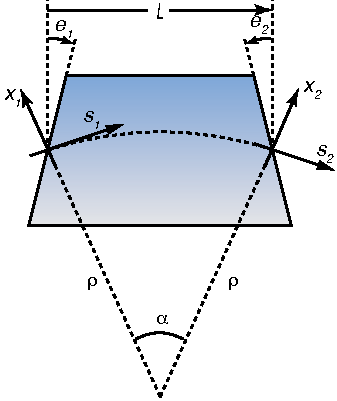
\includegraphics{rbend-coords.pdf}}
  \hspace{1cm}
  \subfigure[sbend]
  {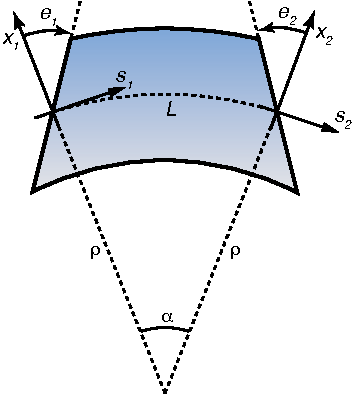
\includegraphics{sbend-coords.pdf}}
  \caption[Coordinate systems for (a) \vn{rbend}\ and (b) \vn{sbend}\ elements.]
{Coordinate systems for (a) \vn{rbend} and (b) \vn{sbend} elements.
For the bends drawn as viewed from ``above'' (viewed from positive $y$),
\vn{g}, \vn{angle}, \vn{rho}, \vn{e1} and \vn{e2} are all positive.}
  \label{f:bend}
\end{figure}

  \begin{description}
  \index{angle}
  \item[angle] \Newline
The total design bend angle. A positive \vn{angle} represents a
bend towards negative $x$ values (see \fig{f:local.coords}).
  \index{e1}\index{e2}
  \item[e1, e2] \Newline
The rotation angle of the entrance pole face is \vn{e1} and at the exit face it is
\vn{e2}. Zero \vn{e1} and \vn{e2} for an \vn{rbend} gives a rectangular magnet
(\fig{f:bend}a). Zero \vn{e1} and \vn{e2} for an \vn{sbend} gives a wedge shaped magnet
(\fig{f:bend}b).  An \vn{sbend} with an \vn{e1} = \vn{e2} = \vn{angle}/2 is equivalent to
an \vn{rbend} with \vn{e1} = \vn{e2} = 0 (see above).  This formula holds for both
positive and negative angles.

Note: The correspondence between \vn{e1} and \vn{e2} and the
corresponding SAD parameters is:
\begin{example}
  e1(Bmad) =  e1(SAD) * angle + ae1(SAD)
  e2(Bmad) =  e2(SAD) * angle + ae2(SAD)
\end{example}
  \index{exact_multipoles}
  \item[exact_multipoles] \Newline
The \vn{exact_multipoles} switch can be set to one of:
\begin{example}
  off                 ! Default
  vertically_pure    
  horizontally_pure  
\end{example}
This switch determines if the multipole fields, both magnetic and electric, and including
the \vn{k1} and \vn{k2} components, are corrected for the finite curvature of the
reference orbit in a bend. See \sref{s:field.exact} for a discussion of what
\vn{vertically} pure versus \vn{horizontally} pure means. Setting \vn{exact_multipoles} to
\vn{vertically_pure} means that the individual $a_n$ and $b_n$ multipole components are
used with the vertically pure solutions
\begin{align}
  \bfB &= \sum_{n = 0}^\infty \left[ \frac{a_n}{n+1} \nabla \phi_n^r + \frac{b_n}{n+1} \nabla \phi_n^i \right] \nonumber
  \bfE &= \sum_{n = 0}^\infty \left[ \frac{a_{en}}{n+1} \nabla \phi_n^i + \frac{b_{en}}{n+1} \nabla \phi_n^r \right]
\end{align}
and if \vn{exact_multipoles} is set to \vn{horizontally_pure} the horizontally pure solutions $\psi_n^r$ and $\psi_n^i$ are
used instead of the vertically pure solutions $\phi_n^r$ and $\phi_n^i$.

To use exact multipoles with PTC based tracking (\sref{c:methods}), the PTC exact model
tracking must be turned on. That is, in the lattice file set:
\begin{example}
  parameter[ptc_exact_model] = T
\end{example}
  \index{fint}\index{fintx}\index{hgapx}\index{hgapx}
  \item[fint, fintx, \Newline hgap, hgapx] \Newline
The field integrals for the entrance and
exit pole faces are give by \vn{fint} and \vn{fintx} respectively
\Begineq
  F_{int} = \int_{pole} \! \! ds \, \frac{B_y(s) \, (B_{y0} - B_y(s))}
  {2 \, H_{gap} \, B_{y0}^2}
  \label{fsbbb}
\Endeq
with a similar equation for \vn{fintx}. In the equation $B_{y0}$ is the field in the
interior of the dipole and $H_{gap}$ is the pole half gap.  The parameters \vn{hgap} and
\vn{hgapx} are the half gaps at the entrance and exit faces. If \vn{fint} or \vn{fintx} is
given without a value then a value of 0.5 is used. If \vn{fint} or \vn{fintx} is not
present, the default value of 0 is used. Note: \mad does not have the \vn{fintx} and
\vn{hgapx} attributes. \mad just assumes that the values are the same for the entrance and
exit faces. For compatibility with \mad, if \vn{fint} is given but \vn{fintx} is not, then
\vn{fintx} is set equal to \vn{fint}. Similarly, \vn{hgapx} will be set to \vn{hgap} if
\vn{hgapx} is not given.

Note: The SAD program uses \vn{fb1+f1} for the entrance fringe and
\vn{fb2+f1} for the exit fringe. The correspondence between the two is
\begin{example}
  fint  * hgap  = (fb1 + f1) / 12
  fintx * hgapx = (fb2 + f1) / 12
\end{example}

\index{Enge function}
\vn{fint} and \vn{hgap} can be related to the Enge function which is sometimes
used to model the fringe field. The Enge function is of the form
\Begineq
  B_y(s) = \frac{B_{y0}}{1 + \exp[P(s)]}
\Endeq
where
\Begineq
  P(s) = C_0 + C_1 \, s + C_2 \, s^2 + C_3 \, s^3 + \, \ldots
\Endeq
The $C_0$ term simply shifts where the edge of the bend is. If all the $C_n$
are zero except for $C_0$ and $C_1$ then 
\Begineq
  C_1 = \frac{1}{2 \,H_{gap} \, F_{int}}
\Endeq
  \index{g}\index{rho}\index{g_err}
  \item[g, g_err, rho] \Newline
The design bending radius which determines the reference coordinate
system is \vn{rho} (see \sref{s:ref}). \vn{g} = 1/\vn{rho} is
the curvature function and is proportional to the design dipole
magnetic field. The true field strength is given by
\vn{g}~+~\vn{g_err} so changing \vn{g_err} leaves the design orbit
unchanged but varies a particle's orbit.
  \index{h1}\index{h2}
  \item[h1, h2] \Newline
The attributes \vn{h1} and \vn{h2} are the curvature of the entrance
and exit pole faces. They are present for compatibility with MAD but
are not yet implemented in terms of tracking and other calculations.
  \index{k1}\index{b1_gradient}
  \item[k1, b1_gradient] \Newline
The normalized and unnormalized quadrupole strength.
  \index{k2}\index{b2_gradient}
  \item[k2, b2_gradient] \Newline
The normalized and unnormalized sextupole strength. 
  \index{l}\index{l_chord}\index{l_arc}
  \item[l, l_arc, l_chord]  \Newline
For compatibility with MAD, for an \vn{rbend}, \vn{l} is the chord
length and not the arc length as it is for an \vn{sbend}.  However,
after reading in a lattice, \bmad will internally convert all
\vn{rbend}s into \vn{sbend}s, additionally, the \vn{l_chord} attribute
will be set to the input \vn{l}, and \vn{l} will be set to the true
path length (see above). Alternatively for an \vn{rbend}, instead of
setting \vn{l}, the \vn{l_arc} attribute can be set to the true arc
length.
  \index{ref_tilt}
  \item[ref_tilt] \Newline
The \vn{ref_tilt} attribute rotates a bend about the longitudinal axis
at the entrance face of the bend. \vn{ref_tilt} = 0 bends the bends
the element in the $-y$ direction. See \fig{f:tilt.bend}. It is
important to understand that \vn{ref_tilt}, unlike the \vn{tilt}
attribute of other elements, bends both the reference orbit along with
the physical element. Note that the MAD \vn{tilt} attribute for bends
is equivalent to the \bmad \vn{ref_tilt}. Bends in \bmad do not have
a \vn{tilt} attribute.
  \end{description}

%---------------

\index{l}
The difference between \vn{rbend} and \vn{sbend} elements
is the way the \vn{l}, \vn{e1}, and \vn{e2} attributes are interpreted.
To ease the bookkeeping burden, after reading in a lattice, \bmad will
internally convert all \vn{rbend}s into \vn{sbend}s. 
This is done using the following transformation on \vn{rbend}s:
\begin{example}
  l_chord(internal) = l(input)
  l(internal) = 2 * asin(l_chord * g / 2) / g
  e1(internal) = e1(input) + theta / 2
  e2(internal) = e2(input) + theta / 2
\end{example}

The attributes \vn{g}, \vn{angle}, and \vn{l} are mutually dependent. If any two are
specified for an element \bmad will calculate the appropriate value
for the third.  After reading in a lattice, \vn{angle} is considered a
dependent variable (\sref{s:depend}).

Since internally all \vn{rbend}s are converted to \vn{sbend}s, if one wants to
vary the \vn{g} attribute of a bend and still keep the bend rectangular, an
overlay (\sref{s:overlay}) can be constructed to maintain the proper face angles.
For example:
\begin{example}
  l_ch = 0.54
  g_in = 1.52
  l_coef = asin(l_ch * g_in / 2) / g_in
  my_bend: rbend, l = l_ch, g = g_in
  my_overlay: overlay = \{my_bend, my_bend[e1]:l_coef, my_bend[e2]:l_coef\}, 
                var = \{g\}, g = g_in
\end{example}
Notice that \vn{l_coef} is just \vn{arc_length/2}.

The \vn{n_ref_pass} attribute are only used
when a bend is part of a \vn{multipass} line and is used to set the
reference geometry of the bend. See section~\sref{s:multipass} for
more details.

In the local coordinate system (\sref{s:ref}), looking from ``above''
(bend viewed from positive $y$), and with \vn{ref_tilt} = 0, a positive
\vn{angle} represents a particle rotating clockwise. In this
case. \vn{g} will also be positive. For counterclockwise rotation,
both \vn{angle} and \vn{g} will be negative but the length \vn{l} is
always positive. Also, looking from above, a positive \vn{e1}
represents a clockwise rotation of the entrance face and a positive
\vn{e2} represents a counterclockwise rotation of the exit face. This
is true irregardless of the sign of \vn{angle} and \vn{g}. Also it is
always the case that the pole faces will be parallel when
\begin{example}
  e1 + e2 = angle
\end{example}

\begin{figure}[tb]
  \centering
  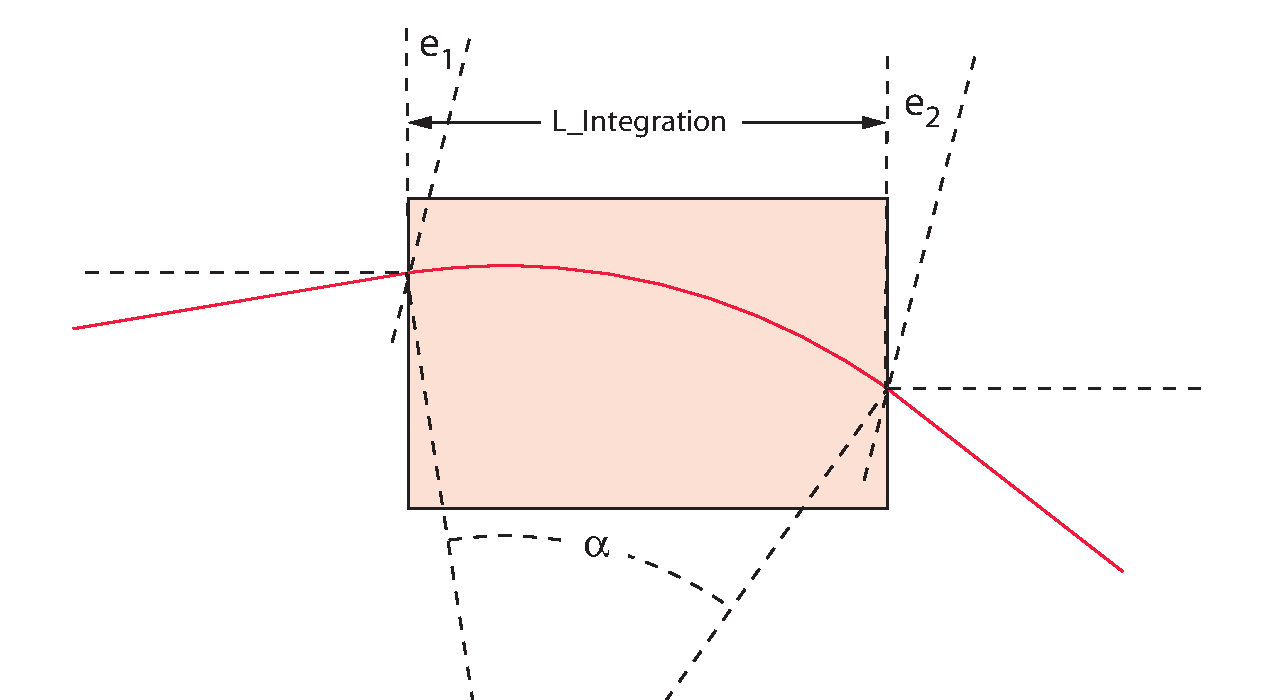
\includegraphics[width=5in]{true-rbend.pdf}
  \caption[True Rbend coordinates]{Coordinate system when \vn{ptc_field_geometry}
is set to \vn{true_rbend}.}
  \label{f:true.rbend}
\end{figure}

Example bend specification:
\begin{example}
  b03w: sbend, l = 0.6, k1 = 0.003, fint  ! gives fint = fintx = 0.5
\end{example}


\vn{ptc_field_geometry} determines how PTC integrates through a bend
if PTC is being used for tracking. Possible values for
\vn{ptc_field_geometry} are:
\begin{example}
  sector      ! Default
  straight
  true_rbend  ! Only valid for rbend elements
\end{example}
For \vn{sector} tracking, the tracking coordinate reference frame is
with respect to the arc of the reference trajectory. For \vn{straight}
tracking the tracking coordinate reference frame is with respect to the
chord line. For a bend where the number of integration steps is large
enough, and where there are no other fields besides the basic dipole
field, the results are the same.  When there are quadrupole or higher
order fields, the fields are expanded about the tracking reference
frame. Since Maxwell's equations must be satisfied, the higher order
fields will differ when tracking with \vn{sector} vs \vn{straight} the
difference in the fields will scale with the inverse of the bending
radius \vn{1/rho}. The above discussion is true for
\vn{ptc_exact_model} set to True, for \vn{ptc_exact_model} set to
False, a simplified sector tracking model is used in all cases.

The \vn{true_rbend} tracking of \vn{ptc_field_geometry} is used only
with \vn{rbend} elements and the entrance and exit faces must be parallel
as shown in \fig{f:true.rbend}. That is
\begin{example}
  e1 + e2 = 0
\end{example}
In this case, the tracking geometry is parallel, to the bend face as
shown in the figure. This can be an advantage in some situations but
\'Etienne Forest discourages use of \vn{true_rbend} due to complications
of how to handle the reference frames. In particular, how to handle
the reference frames is problematic when you have more than one of
them in a row.

%-----------------------------------------------------------------
\section{Capillary}
\label{s:capillary}
\index{capillary|hyperbf}

A \vn{capillary} element is a glass tube that is used to focus x-ray
beams.

General \vn{capillary} attributes are:
\begin{center}
\tt
\begin{tabular}{llll} \toprule
  {\sl Attribute Class}      & Section          & {\sl Attribute Class}      & Section         \\ \midrule
  Aperture limits            & \ref{s:limit}    & Offsets, Pitches \& Tilt   & \ref{s:offset}  \\ 
  Capillary Wall             & \ref{s:wall}     & Reference energy           & \ref{s:energy}  \\
  Custom Attributes          & \ref{s:cust.att} & Tracking \& transfer map   & \ref{c:methods} \\ 
  Description strings        & \ref{s:alias}    &                            &                 \\
  \bottomrule
\end{tabular}
\end{center}
\toffset
See \sref{s:list.capillary} for a full list of element attributes.

\index{critical_angle_factor|hyperbf}
Attributes specific to a \vn{capillary} element are:
\begin{example}
  critical_angle_factor = <Real>    ! Critical angle * Energy (rad * eV)
\end{example}

The critical angle above which photons striking the capillary surface are
refracted into the capillary material scales as 1/Energy. The
constant of critical angle * energy is given by the \vn{critical_angle_factor}.

The inside wall of a capillary is defined using the same syntax used
to define the chamber wall for other elements (\sref{s:wall}).

The length of the capillary is a dependent variable and is given by
the value of \vn{s} of the last wall cross-section
(\sref{s:wall.capillary}).

%-----------------------------------------------------------------
\section{Collimators: Ecollimator and Rcollimator} 
\label{s:col}
\index{ecollimator|hyperbf}
\index{rcollimator|hyperbf}

An \vn{ecollimator} is a drift with elliptic collimation. An
\vn{rcollimator} is a drift with rectangular collimation.

General \vn{ecollimator} and \vn{rcollimator} attributes are:
\begin{center}
\tt
\begin{tabular}{llll} \toprule
  {\sl Attribute Class}      & Section          & {\sl Attribute Class}      & Section          \\ \midrule
  Aperture limits            & \ref{s:limit}    & Overlapping Fields         & \ref{s:overlap}  \\
  Chamber wall               & \ref{s:wall}     & Reference energy           & \ref{s:energy}   \\
  Custom Attributes          & \ref{s:cust.att} & Superposition              & \ref{s:super}    \\
  Description strings        & \ref{s:alias}    & Symplectify                & \ref{s:symp}     \\
  Hkick \& Vkick             & \ref{s:kick}     & Field Maps                 & \ref{s:fieldmap} \\
  Length                     & \ref{s:l}        & Tracking \& transfer map   & \ref{c:methods}  \\
  Offsets, Pitches \& Tilt   & \ref{s:offset}   &                            &                  \\
  \bottomrule
\end{tabular}
\end{center}
\toffset

Note: Collimators are the exception to the rule that the aperture is
independent of any \vn{tilt}s. See \sref{s:limit} for more
details. Additionally, the default setting of
\vn{offset_moves_aperture} is \vn{True} for collimators (\sref{s:offset.ap}).

Example:
\begin{example}
  d21: ecollimator, l = 4.5, x_limit = 0.09/2, y_limit = 0.05/2
\end{example}

%-----------------------------------------------------------------
\section{Crystal}
\label{s:crystal}
\index{crystal|hyperbf}

\begin{figure}[tb]
  \centering
  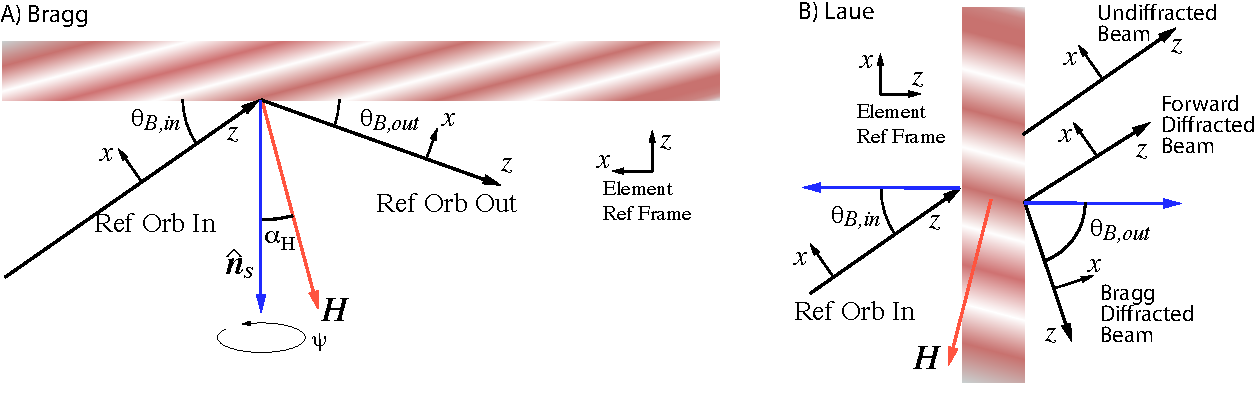
\includegraphics[width=5in]{crystal-ele.pdf}
  \caption[Crystal element geometry.]
{Crystal element geometry.  A) Geometry for Bragg diffraction. The
geometry shown is for \vn{ref_tilt} = 0 (reference trajectory in the
$x$-$z$ plane). The angle $\alpha_H$ (\vn{alpha_angle}) is the angle
of the $\bfH$ vector with respect to the surface normal $\bfhat
n$. For $\psi$ (\vn{psi_angle}) zero, the incoming reference orbit,
the outgoing reference orbit, $\bfhat n$, and $\bfH$ are all
coplanar. B) Geometry for Laue diffraction. In this case there are
three outgoing beams: The Bragg diffracted beam, the forward
diffracted beam, and the undiffracted beam.}
  \label{f:crystal}
\end{figure}

A \vn{crystal} element represents a crystal used for photon diffraction.

General \vn{crystal} attributes are:
\begin{center}
\tt
\begin{tabular}{llll} \toprule
  {\sl Attribute Class}      & Section          & {\sl Attribute Class}      & Section         \\ \midrule
  Aperture limits            & \ref{s:limit}    & Surface Properties         & \ref{s:s.curve} \\ 
  Custom Attributes          & \ref{s:cust.att} & Symplectify                & \ref{s:symp}    \\
  Description strings        & \ref{s:alias}    & Offsets, Pitches \& Tilt   & \ref{s:offset}  \\
  Reference energy           & \ref{s:energy}   & Tracking \& transfer map   & \ref{c:methods} \\
  \bottomrule
\end{tabular}
\end{center}
\toffset
See \sref{s:list.crystal} for a full list of element attributes.

\index{psi_angle}
\index{b_param}\index{bragg_angle}\index{crystal_type}
\index{follow_diffracted_beam}\index{thickness}
Attributes specific to a \vn{crystal} element are:
\begin{example}
  b_param            = <Real>       ! b parameter
  crystal_type       = <String>     ! Crystal material (\sref{s:cryst.list}) and reflection plane.
  psi_angle          = <Real>       ! Rotation of H-vector about the surface normal.
  thickness          = <Real>       ! Thickness of crystal for Laue diffraction.
  ref_orbit_follows  = <which_beam> ! Reference orbit aligned with what outgoing beam?
\end{example}

\index{bragg_angle_in}\index{bragg_angle_out}\index{alpha_angle}
\index{tilt_corr}\index{d_spacing}\index{v_unitcell}\index{l}
\index{ref_wave_length}\index{dbragg_angle_de}
\index{pendellosung_period_sigma}\index{pendellosung_period_pi}
Dependent variables (\sref{s:depend}) specific to a \vn{crystal} element are:
\begin{example}
  alpha_angle                ! Angle of H-vector with respect to the surface normal.
  bragg_angle                ! Nominal Bragg angle at the reference wave length. 
  bragg_angle_in             ! Angle between incoming beam and surface.
  bragg_angle_out            ! Angle between outgoing beam and surface.
  d_spacing                  ! Lattice plane spacing. 
  darwin_width_pi            ! Darwin width for pi polarized light (radians).
  darwin_width_sigma         ! Darwin width for sigma polarized light (radians).
  dbragg_angle_de            ! Variation of the Bragg angle with energy (radians/eV).
  l                          ! Length of reference orbit.
  pendellosung_period_pi     ! Pendellosung period for pi polarized light.
  pendellosung_period_sigma  ! Pendellosung period for sigma polarized light.
  ref_wavelength             ! Reference wavelength (\sref{s:energy}). Dependent attribute (\sref{s:depend}).
  ref_cap_gamma              ! \(\Gamma\) at the reference wavelength.
  tilt_corr                  ! Tilt correction due to a finite psi_angle.
  v_unitcell                 ! Unit cell volume. 
\end{example}

The \vn{crystal_type} attribute defines the crystal material and
diffraction lattice plane. The syntax is \vn{"ZZZ(ijk)"} where \vn{ZZZ}
is the material name and \vn{ijk} are the Miller
indices for the diffraction plane. For example,
\begin{example}
  b_cryst1: crystal, crystal_type = "Si(111)", b_param = -1, ...
\end{example}
The atomic formula is case sensitive so, for example, \vn{"SI(111)"}
is not acceptable. The list of known crystal materials is given in
\sref{s:cryst.list}. Given the \vn{crystal_type}, the spacing between
lattice planes (\vn{d_spacing}), the unit cell volume
(\vn{v_unitcell}), and the structure factor\cite{b:batterman} values
can be computed.

The \vn{b_param} is the standard asymmetry factor
\Begineq
  b = \frac{\sin(\alpha_H + \theta_B)}{\sin(\alpha_H - \theta_B)} 
  \label{batat}
\Endeq
where $\theta_B$ is the Bragg angle (\vn{bragg_angle}) 
\Begineq
  \theta_B = \sin^{-1} \left( \frac{\lambda}{2 \, d} \right)
  \label{tsl2d}
\Endeq
and $\alpha_H$ (\vn{alpha_angle}) is the angle of the reciprocal
lattice $\bfH$ vector with respect to the surface normal as shown in
\fig{f:crystal}A.  If \vn{b_param} is set to -1 then there is
Bragg reflection and \vn{alpha_H} is zero. If \vn{b_param} is set to 1
then there is Laue diffraction again with \vn{alpha_H} zero. With the
orientation shown in \fig{f:crystal}A, \vn{alpha_H} is positive.

The \vn{thickness} parameter is used with Laue diffraction only.

The \vn{ref_orbit_follows} parameter sets how the outgoing reference
orbit is constructed. This is only relevant with Laue diffraction.
The possible settings of this parameter are:
\begin{example}
  bragg_diffracted
  forward_diffracted
  undiffracted
\end{example}
The geometry of this situation is shown in \fig{f:crystal}B. The
reference orbit for the \vn{undiffracted} beam is just a straight line
extension of the incoming reference trajectory. This trajectory is
that trajectory that photons whose energy is far from the Bragg
condition (that is, far from the reference energy) will follow. The
\vn{forward_diffracted} reference orbit is parallel to the
\vn{undiffracted} trajectory and is the trajectory of the forward
diffracted photons whose energy is the reference energy and whose
incoming orbit is on the incoming reference trajectory. Finally, the
\vn{bragg_diffracted} reference orbit is the backward diffracted orbit.

Note: Changing the setting of \vn{ref_orbit_follows} will change the
reference orbit downstream of the crystal which, in turn, will change
the placement all downstream elements.

The value of the element reference orbit length \vn{l} is calculated
by \bmad. \vn{L} will be zero for Bragg diffraction. For Laue
diffraction, \vn{l} will depend upon the crystal \vn{thickness} and
the setting of \vn{ref_orbit_follows}.

If \vn{psi_angle} is zero, the incoming reference orbit, the outgoing
reference orbit, $\bfhat n$ and $\bfH$ are all coplanar. A non-zero
\vn{psi_angle} Rotates the $\bfH$ vector around the $+\bfhat x$ axis
of the \vn{Element Reference Frame} (See \fig{f:crystal}A).

To keep the outgoing reference trajectory independent of the value of
\vn{psi_angle}, the crystal will be automatically tilted by the
appropriate ``tilt correction'' \vn{tilt_corr}. The calculation of
\vn{tilt_corr} is outlined in \sref{s:crystal.trans}. \vn{tilt_corr}
will be zero if \vn{psi_angle} is zero.

The reference trajectory for a Bragg \vn{crystal} is that of a zero
length bend (\sref{s:mirror.coords}) and hence the length (\vn{l})
parameter of a crystal is fixed at zero. The orientation of the
reference trajectory with respect to the crystal surface is specified
by the incoming Bragg angle \vn{bragg_angle_in} ($\theta_{g,in}$) and
outgoing Bragg angle \vn{bragg_angle_out} ($\theta_{g,out}$) as shown
in \fig{f:crystal}A. These angles are computed from the photon
reference energy and the other crystal parameters such that a photon
with the reference energy traveling along the reference trajectory
will be in the center of the Darwin curve (\sref{s:crystal.tracking}).

Notice that due to refraction at the surface, the computed
\vn{bragg_angle} from \Eq{tsl2d} will deviate slightly from the
average of \vn{bragg_angle_in} and \vn{bragg_angle_out}.

The reference trajectory in the global coordinate system
(\sref{s:global}) is determined by the value of the \vn{ref_tilt}
parameter along with the value of \vn{bragg_angle_in} +
\vn{bragg_angle_out}. These bragg angles take into account refraction
so that the reference trajectory downstream of the crystal will be
properly centered with respect to the reference photon. A positive
\vn{bragg_angle_in} + \vn{bragg_angle_out} bends the reference
trajectory in the same direction as a positive \vn{g} for a bend
element. The

A \vn{crystal} may be offset and pitched (\ref{s:offset}). The incoming
local reference coordinates are used for these misalignments. 

When a crystal is bent (\sref{s:s.curve}), the $\bfH$ vector is
assumed follow the surface curvature. That is, it is assumed that the
lattice planes are curved by the bending.

Example:
\begin{example}
  crystal_ele: crystal, crystal_type = 'Si(111)', b_param = -1
\end{example}

The \vn{darwin_width_sigma} and \vn{darwin_width_pi} parameters are
the computed Darwin width, in radians, for sigma and pi polarized
light respectively. Here the Darwin width $d\theta_D$ is defined as
the width at the $\eta = \pm 1$ points
(cf.~Batterman\cite{b:batterman} Eq (32))
\Begineq
  d\theta_D = \frac{2 \, \Gamma \, |P| \, \text{Re} \! \left( [F_H \, F_{\Hbar}]^{1/2} \right)}
                 {|b|^{1/2} \, \sin\theta_{tot}}
\Endeq
where
\begin{example}
  \(\theta_{tot}\) = bragg_angle_in + bragg_angle_out 
\end{example}

The \vn{pendellosung_period_sigma} and \vn{pendellosung_period_pi} are
the pendellosung periods for Laue diffraction. If the crystal is set up for
Bragg diffraction then the values for these parameters will be set to zero.

The \vn{dbragg_angle_de} parameter is the variation in Bragg angle
with respect to the photon energy and is given by the formula
\Begineq
  \frac{d\theta_B}{dE} = -\frac{\lambda}{2 \, d \, E \, \cos( \theta_B )}
\Endeq

%-----------------------------------------------------------------
\section{Custom}
\label{s:custom}
\index{custom|hyperbf}

A \vn{custom} element is an element whose properties are defined
outside of the standard \bmad subroutine library. That is, to use a
custom element, some programmer must write the appropriate custom
routines which are then linked with the \bmad subroutines into a
program. \bmad will call the custom routines at the appropriate time
to do tracking, transfer matrix calculations, etc. See the programmer
who wrote the custom routines for more details! See
\sref{s:custom.ele} on how to write custom routines.

General \vn{custom} attributes are:
\begin{center}
\tt
\begin{tabular}{llll} \toprule
  {\sl Attribute Class}      & Section           & {\sl Attribute Class}      & Section         \\ \midrule
  Aperture limits            & \ref{s:limit}     & Length                     & \ref{s:l}       \\
  Chamber wall               & \ref{s:wall}      & Offsets, pitches \& tilt   & \ref{s:offset}  \\
  Custom Attributes          & \ref{s:cust.att}  & Reference energy           & \ref{s:energy}  \\ 
  Description strings        & \ref{s:alias}     & Superposition              & \ref{s:super}   \\
  Field Maps                 & \ref{s:fieldmap}  & Symplectify                & \ref{s:symp}    \\
  Fringe fields              & \ref{s:fringe}    & Tracking \& transfer map   & \ref{c:methods} \\ 
  Is_on                      & \ref{s:is.on}     &                            &                 \\ 
  \bottomrule
\end{tabular}
\end{center}
\toffset
See \sref{s:list.custom} for a full list of element attributes.

\index{tracking_method}\index{mat6_calc_method}\index{field_calc}
As an alternative to defining a custom element, standard elements can
be ``customized'' by setting one or more of the following attributes
to \vn{custom}:
\begin{example}
  tracking_method       \sref{s:tkm}
  mat6_calc_method      \sref{s:xfer}
  field_calc            \sref{s:integ}
  aperture_type         \sref{s:limit}
\end{example}

As with a custom element, setting one of these attributes to
\vn{custom} necessitates the use of custom code to implement the
corresponding calculation.

\index{delta_e}
\index{val1,  ..., Val12}
Attributes specific to a \vn{custom} element are
\begin{example}
  val1, ..., val12 = <Real>  ! Custom values 
  delta_e          = <Real>  ! Change in energy.
\end{example}

\vn{delta_e} is the energy gain of the {\it reference} particle
between the starting edge of the element and the ending edge.

Example:
\begin{example}
  c1: custom, l = 3, val4 = 5.6, val12 = 0.9, descrip = 'params.dat'
\end{example}
In this example the \vn{descrip} string is being used to specify a
file that contains parameters for the element.

%-----------------------------------------------------------------
\section{Detector}
\label{s:detector}
\index{detector|hyperbf}

A \vn{detector} element is used to detect particles and X-rays.  A
\vn{detector} is modeled as a grid of pixels which detect particles and x-rays
impinging upon them.

General \vn{detector} element attributes are:
\begin{center}
\tt 
\begin{tabular}{llll} \toprule
  {\sl Attribute Class}      & Section           & {\sl Attribute Class}      & Section         \\ \midrule
  Aperture limits            & \ref{s:limit}     & Offsets, pitches \& tilt   & \ref{s:offset}  \\
  Chamber Wall               & \ref{s:wall}      & Reference energy           & \ref{s:energy}  \\
  Custom Attributes          & \ref{s:cust.att}  & Superposition              & \ref{s:super}   \\
  Description strings        & \ref{s:alias}     & Tracking \& transfer map   & \ref{c:methods} \\
  Detector Geometry          & \ref{s:surf.grid} &                            &                 \\
  \bottomrule
\end{tabular}
\end{center}
\toffset
See \sref{s:list.detector} for a full list of element attributes.

The detector pixels are are arranged in a rectangular grid (\sref{s:surf.grid}). 

\index{aperture_type}
The \vn{aperture_type} (\sref{s:limit}) parameter of a
\vn{detector} will default to \vn{auto} which will set the
aperture limits to define a rectangular aperture that just cover the
clear area of the plate.

Example:
\begin{example}
  det: detector, surface = \{grid = 
          \{ix_bounds = (-4,5), iy_bounds = (-10,10), dr = (0.01, 0.01)\}\}
\end{example}
This example defines a detector with 1~cm x 1~cm pixels.

%-----------------------------------------------------------------
\section{Diffraction_Plate}
\label{s:diff.plate}
\index{diffraction_plate|hyperbf}

A \vn{diffraction_plate} element is a flat surface oriented, more or
less, transversely to a x-ray beam through which photon can travel. A
\vn{diffraction_plate} can be used, for example, to model a Fresnel
zone plate or Young's double slits. A \vn{diffraction_plate} element
is used in places where diffraction effects must be taken into
account. This is in contrast to setting an aperture attribute
(\sref{s:limit} for other elements where diffraction effects are
ignored.

A \vn{diffraction_plate} element is similar to a \vn{mask}
(\sref{s:mask}) element except that with a \vn{mask} element coherent
effects are ignored. Additionally, a \vn{mask} element can be used
with charged particles while a \vn{diffraction_plate} cannot.

General \vn{diffraction_plate} element attributes are:
\begin{center}
\tt 
\begin{tabular}{llll} \toprule
  {\sl Attribute Class}      & Section          & {\sl Attribute Class}      & Section         \\ \midrule
  Aperture limits            & \ref{s:limit}    & Offsets, pitches \& tilt   & \ref{s:offset}   \\ 
  Custom Attributes          & \ref{s:cust.att} & Mask geometry              & \ref{s:wall}    \\
  Description strings        & \ref{s:alias}    & Reference energy           & \ref{s:energy}  \\
  Is_on                      & \ref{s:is.on}    & Tracking \& transfer map   & \ref{c:methods} \\
  \bottomrule
\end{tabular}
\end{center}
\toffset
See \sref{s:list.diffraction.plate} for a full list of element attributes.

\index{mode}\index{field_scale_factor}
Attributes specific to a \vn{diffraction_plate} element are:
\begin{example}
  mode               = <Type>   ! Reflection or transmission
  field_scale_factor = <Real>   ! Factor to scale the photon field
  ref_wavelength                ! Reference wavelength (\sref{s:energy}). Dependent attribute (\sref{s:depend}).
\end{example}

The \vn{mode} switch sets whether X-rays are transmitted through the
\vn{diffraction_plate} or or reflected. Possible values for the
\vn{mode} switch are:
\begin{example}
  reflection
  transmission        ! Default
\end{example}

The geometry of the plate, that is, where the openings (in
transmission mode) or reflection regions are, is defined using the
``wall'' attribute. See (\sref{s:wall}) for more details.

In transmission mode, a \vn{diffraction_plate} is nominally orientated
transversely to the beam. Like all other elements, the
\vn{diffraction_plate} can be reoriented using the element's offsets,
pitches and tilt attributes (\sref{s:offset}).

\index{aperture_type}
The \vn{aperture_type} (\sref{s:limit}) parameter of a
\vn{diffraction_plate} will default to \vn{auto} which will set the
aperture limits to define a rectangular aperture that just cover the
clear area of the plate.

\index{field_scale_factor}
The \vn{field_scale_factor}, if set to a non-zero value (zero is the
default) will be used to scale the field of photons as they pass through
the \vn{diffraction_plate} element:
\begin{example}
  field -> field * field_scale_factor
\end{example}
Scaling is useful since the electric field of photons traveling through a
\vn{diffraction_plate} are renormalized (see \Eqs{eeo4p} and
\eq{eek4p}). This can lead to large variation of the photon field and
can, for example, make visual interpretation of plots of field verses
longitudinal position difficult to interpret. \vn{field_scale_factor}
can be used to keep the field more or less constant.

A \vn{diffraction_plate} that is ``turned off'' (\vn{is_on} attribute
set to False), does not diffract at all and transmits through all
the light incident on it.

Example:
\begin{example}
  fresnel: diffraction_plate, wall = \{...\}
\end{example}

%-----------------------------------------------------------------
\section{Drift}
\label{s:drift}
\index{drift|hyperbf}

A \vn{drift} element is a space free and clear of any fields.

General \vn{drift} attributes are:
\begin{center}
\tt
\begin{tabular}{llll} \toprule
  {\sl Attribute Class}      & Section          & {\sl Attribute Class}      & Section         \\ \midrule
  Aperture limits            & \ref{s:limit}    & Offsets, pitches \& tilt   & \ref{s:offset}  \\
  Custom Attributes          & \ref{s:cust.att} & Reference energy           & \ref{s:energy}  \\ 
  Description strings        & \ref{s:alias}    & Symplectify                & \ref{s:symp}    \\ 
  Length                     & \ref{s:l}        & Tracking \& transfer map   & \ref{c:methods} \\ 
  \bottomrule
\end{tabular}
\end{center}
\toffset
See \sref{s:list.drift} for a full list of element attributes.

Example:
\begin{example}
  d21: drift, l = 4.5
\end{example}

Note: If a chamber wall (\sref{s:wall}) is needed for a field free
space, use a \vn{pipe} element instead of a \vn{drift} [a wall for a
drift is not allowed due to the way drifts are treated with
superposition. That is, drifts ``disappear'' when superimposed
upon. (\sref{s:super})].

%-----------------------------------------------------------------
\section{E_Gun}
\label{s:e.gun}
\index{e_gun|hyperbf}

An \vn{e_gun} element represents an electron gun and encompasses a
region starting from the cathode were the electrons are generated.
General \vn{e_gun} attributes are:
\begin{center}
\tt
\begin{tabular}{llll} \toprule
  {\sl Attribute Class}      & Section           & {\sl Attribute Class}      & Section           \\ \midrule
  Aperture limits            & \ref{s:limit}     & Mag \& Elec multipoles     & \ref{s:multip}    \\
  Chamber wall               & \ref{s:wall}      & Offsets, pitches \& tilt   & \ref{s:offset}    \\ 
  Custom attributes          & \ref{s:cust.att}  & Overlapping Fields         & \ref{s:overlap}   \\
  Description strings        & \ref{s:alias}     & Reference energy           & \ref{s:energy}    \\ 
  Field autoscaling          & \ref{s:autoscale} & Symplectify                & \ref{s:symp}      \\
  Hkick \& Vkick             & \ref{s:kick}      & Field Maps                 & \ref{s:fieldmap}  \\
  Is_on                      & \ref{s:is.on}     & Tracking \& transfer map   & \ref{c:methods}   \\ 
  Length                     & \ref{s:l}         &                            &                   \\
  \bottomrule
\end{tabular}
\end{center}
\toffset
See \sref{s:list.e.gun} for a full list of element attributes.

The attributes specific to an \vn{e_gun} are 
\index{voltage}\index{voltage_err}
\index{gradient}\index{gradient_err}
\begin{example}
  gradient       = <Real>    ! Gradient.
  gradient_err   = <Real>    ! Gradient error.
  phi0           = <Real>    ! Phase (rad/2\(\pi\)) of the reference particle with 
                             !   respect to the RF. phi0 = 0 is on crest.
  phi0_err       = <Real>    ! Phase error (rad/2\(\pi\))
  rf_frequency   = <Real>    ! Frequency of the RF field.
  voltage        = <Real>    ! Voltage. Dependent attribute (\sref{s:depend}). 
  voltage_err    = <Real>    ! Voltage error. Dependent attribute (\sref{s:depend}). 
\end{example}

The \vn{voltage} is simply related to the \vn{gradient} via the element length \vn{l}:
\begin{example}
  voltage = gradient * l
\end{example}
If the \vn{voltage} is set to a non-zero value, the length \vn{l} must also be non-zero to
keep the gradient finite.  A particle with the charge as the reference particle will have
a positive energy gain if the \vn{voltage} and \vn{gradient} are positive and vice versa.

\index{phi0_autoscale}\vn{field_autoscale}
The \vn{voltage} and \vn{gradient} are scaled by \vn{field_autoscale} and, if there is a
finite \vn{rf_frequency}, the phase of the frequency is shifted by \vn{phi0_autoscale} as
discussed in Section~\sref{s:autoscale}. Autoscaling can be toggled on/off by using the
\vn{autoscale_phase} and \vn{autoscale_amplitude} toggles.

An \vn{e_gun} may either be DC if the \vn{rf_frequency} component is zero of AC if
not. For an AC \vn{e_gun}, the phase of the \vn{e_gun}, The phase $\phi_{\text{ref}}$
is 
\begin{example} 
  \(\phi_{\text{ref}}\) = phi0 + phi0_err + phi0_autoscale 
\end{example}

\index{marker}\index{null_ele}
Electrons generated at the cathode can have zero initial momentum and
this presents a special problem (\sref{s:energy}). As a result, the
use of \vn{e_gun} elements are restricted and they can only be used in
a ``linear'' (non-recirculating) lattice branch. Only one \vn{e_gun}
can be present in a lattice branch and, if it is present, it must be,
except for possibly \vn{marker} or \vn{null_ele} elements, the first
element in any branch.
 
Note: In order to be able to avoid problems with a zero reference
momentum at the beginning of the \vn{e_gun}, the reference momentum
and energy associated with an \vn{e_gun} element is calculated as
outlined in Section~\sref{s:energy}. Additionally, the reference
momentum at the exit end of the \vn{e_gun}, that is \vn{p0c}, must be
non-zero. Thus, for example, if \vn{p0c} is zero at the start of the
lattice, the \vn{e_gun} voltage must be non-zero. 

Additionally, in order to be able to avoid problems with a zero reference momentum at the
beginning of the \vn{e_gun}, absolute time tracking (\sref{s:rf.time}) is always used in
an \vn{e_gun} element independent of the setting of \vn{parameter[absolute_time_tracking]}
(\sref{s:param}).

Note: The default \vn{tracking_method} (\sref{s:tkm}) setting for an
\vn{e_gun} is \vn{time_runge_kutta} and the default
\vn{mat6_calc_method} is \vn{tracking}.

In this example the field of an e_gun is given by a grid of field
values (\sref{s:grid.field}):
\begin{example}
  apex: e_gun, l = 0.23, field_calc = fieldmap, rf_frequency = 187e6, 
                grid_field = call::apex_gun_grid.bmad
\end{example}
with the file \vn{apex_gun_grid.bmad} being:
\begin{example}
  \{
    m = 0, harmonic = 1,
    master_scale = voltage,
    geometry = rotationally_symmetric_rz,
    r0 = (0, 0),
    dr = (0.001, 0.001),
    pt(0,0) = ( (0, 0), (0, 0), (1, 0),  (0, 0), (0, 0), (0, 0)),
    pt(0,1) = ( (0, 0), (0, 0), (0.99, 0),  (0, 0), (0, 0), (0, 0)),
    ... \}
\end{example}

%-----------------------------------------------------------------
\section{ELseparator}
\label{s:elsep}
\index{elseparator|hyperbf}

An \vn{elseparator} is an electrostatic separator.

General \vn{elseparator} attributes are:
\begin{center}
\tt
\begin{tabular}{llll} \toprule
  {\sl Attribute Class}      & Section           & {\sl Attribute Class}      & Section          \\ \midrule
  Aperture limits            & \ref{s:limit}     & Mag \& Elec multipoles     & \ref{s:multip}   \\
  Chamber wall               & \ref{s:wall}      & Offsets, pitches \& tilt   & \ref{s:offset}   \\
  Custom Attributes          & \ref{s:cust.att}  & Overlapping Fields         & \ref{s:overlap}  \\
  Description strings        & \ref{s:alias}     & Reference energy           & \ref{s:energy}   \\ 
  Fringe Fields              & \ref{s:fringe}    & Superposition              & \ref{s:super}    \\
  Hkick \& Vkick             & \ref{s:kick}      & Symplectify                & \ref{s:symp}     \\
  Is_on                      & \ref{s:is.on}     & Field Maps                 & \ref{s:fieldmap} \\  
  Length                     & \ref{s:l}         & Tracking \& transfer map   & \ref{c:methods}  \\ 
  \bottomrule
\end{tabular}
\end{center}
\toffset
See \sref{s:list.elseparator} for a full list of element attributes.

\index{gap}
\index{e_field}
\index{voltage}
Attributes specific to an \vn{elseparator} element are:
\begin{example}
  gap = <Real> ! Distance between electrodes
  voltage      ! Voltage between electrodes. This is a settable dependent variable (\sref{s:depend}).
  e_field      ! Electric field. This is a settable dependent variable (\sref{s:depend}).
\end{example}

\index{hkick}
\index{vkick}
For an \vn{elseparator}, the kick for a positively charged particle, with the magnitude of
the charge that is the same as the reference particle (set by \vn{parameter[particle]}
\sref{s:param}), is determined by \vn{hkick} and \vn{vkick}. The kick for a negatively
charged particle is opposite this. The \vn{gap} for an \vn{Elseparator} is used to compute
the voltage for a given kick
\begin{example}
  e_field (V/m) = sqrt(hkick^2 + vkick^2) * P0 * c_light / L
  voltage (V) = e_field * gap
\end{example}

Example:
\begin{example}
  h_sep: elsep, l = 4.5, hkick = 0.003, gap = 0.11
\end{example}

%-----------------------------------------------------------------
\section{EM_Field}
\label{s:em.field}
\index{em_field|hyperbf}

An \vn{em_field} element can contain general electro-magnetic (EM)
fields. Both AC and DC fields are accommodated.  General \vn{em_field}
attributes are:
\begin{center}
\tt
\begin{tabular}{llll} \toprule
  {\sl Attribute Class}      & Section           & {\sl Attribute Class}      & Section         \\ \midrule
  Aperture limits            & \ref{s:limit}     & Length                     & \ref{s:l}       \\ 
  Chamber wall               & \ref{s:wall}      & Offsets, pitches \& tilt   & \ref{s:offset}  \\
  Custom Attributes          & \ref{s:cust.att}  & Reference energy           & \ref{s:energy}  \\
  Description strings        & \ref{s:alias}     & Superposition              & \ref{s:super}   \\
  Field Maps                 & \ref{s:fieldmap}  & Symplectify                & \ref{s:symp}    \\
  Hkick \& Vkick             & \ref{s:kick}      & Tracking \& transfer map   & \ref{c:methods} \\ 
  Is_on                      & \ref{s:is.on}     &                            &                 \\
  \bottomrule
\end{tabular}
\end{center}
\toffset
See \sref{s:list.em.field} for a full list of element attributes.

\vn{em_field} elements will be created when elements are superimposed (\sref{s:super}) and there is
no other suitable element class.

%-----------------------------------------------------------------
\section{Fiducial}
\label{s:fiducial}
\index{fiducial|hyperbf}

A \vn{fiducial} element is used to fix the position and orientation of
the reference orbit within the global coordinate system at the
location of the \vn{fiducial} element. A \vn{fiducial} element will
affect the reference orbit both upstream and downstream of the element.

General \vn{fiducial} element attributes are:
\begin{center}
\tt
\begin{tabular}{llll} \toprule
  {\sl Attribute Class}      & Section           & {\sl Attribute Class}      & Section         \\ \midrule
  Aperture limits            & \ref{s:limit}     & Reference energy           & \ref{s:energy}  \\
  Custom Attributes          & \ref{s:cust.att}  & Superposition              & \ref{s:super}   \\
  Description strings        & \ref{s:alias}     & Tracking \& transfer map   & \ref{c:methods} \\ 
  \bottomrule
\end{tabular}
\end{center}
\toffset
See \sref{s:list.fiducial} for a full list of element attributes.

\index{origin_ele}\index{origin_ele_ref_pt}
\index{x_origin}\index{y_origin}
\index{z_origin}\index{theta_origin}
\index{phi_origin}\index{psi_origin}
Attributes specific to a \vn{fiducial} elements are:
\begin{example}
  origin_ele        = <Name>     ! Reference element.
  origin_ele_ref_pt = <location> ! Reference pt on reference ele.
  dx_origin         = <Real>     ! x-position offset
  dy_origin         = <Real>     ! y-position offset
  dz_origin         = <Real>     ! z-position offset
  dtheta_origin     = <Real>     ! orientation angle offset.
  dphi_origin       = <Real>     ! orientation angle offset.
  dpsi_origin       = <Real>     ! orientation angle offset.
\end{example}

For tracking purposes, the \vn{fiducial} element is considered to be a
zero length marker. That is, the transfer map through a \vn{fiducial}
element is the unit map.

A \vn{fiducial} element sets the reference orbit of itself and of the
elements, both upstream and downstream, around it. This can be thought
of as a two step process. The first step is to determine the global
coordinates of the \vn{fiducial} element itself, and the second step is
to shift the coordinates of the elements around it.

The floor coordinates of the \vn{fiducial} element are determined
starting with an \vn{origin_ele} element. If \vn{origin_ele} is not
specified, the origin of the global coordinates (\sref{s:global} is
used. If the \vn{origin_ele} has a finite length, the reference point
may be chosen using the \vn{origin_ele_ref_pt} attribute which
may be set to one of
\begin{example}
  entrance_end
  center         ! Default
  exit_end
\end{example}

Once the origin reference position is determined, the reference
position of the \vn{fiducial} element is calculated using the offset
attributes 
\begin{example}
  [dx_origin,  dy_origin,  dz_origin]
  [dtheta_origin,  dphi_origin,  dpsi_origin]
\end{example}
The transformation between origin and fiducial positions is given in
\sref{s:patch.coords}.

\index{flexible patch}\index{patch}
Once the position of the \vn{fiducial} element is calculated, all
elements of the lattice branch the \vn{fiducial} element is contained
in, {\em both} the upstream and downstream elements, are shifted so
that everything is consistent. That is, the \vn{fiducial} element
orients the entire lattice branch. The exception here is that if there
are \vn{flexible} \vn{patch} elements (\sref{s:patch}) in the lattice
branch, the \vn{fiducial} element will only determine the positions up
to the \vn{flexible} \vn{patch} element. 

Example: A lattice branch with elements 0 through 103 has a
\vn{fiducial} element at position 34 and a \vn{flexible} \vn{patch} at
position 67. In this case the \vn{fiducial} element will determine the
reference orbit for elements 0 through 66.

Rules: 
  \begin{itemize}
  \item
If an \vn{origin_ele} is specified, the position of this element must
to calculated before the the position of the \vn{fiducial} element is
calculated (\sref{s:ref}). This means, the \vn{origin_ele} must be in
a prior lattice branch from the branch the \vn{fiducial} element is in
or the \vn{origin_ele} in the same branch as the \vn{fiducial} element
but is positioned upstream from the \vn{fiducial} element and there is
a \vn{flexible} \vn{patch} in between the two elements.
  \item
If a \vn{fiducial} element affects the position of element 0 in the
lattice branch (that is, there are no flexible \vn{patch} elements
in between), any positioning of element 0 via \vn{beginning} or
\vn{line parameter} statements (\sref{s:beginning}) are ignored.
  \item
\vn{Fiducial} elements must not over constrain the lattice geometry.
For example, two \vn{fiducial} elements may not appear in the same
lattice branch unless separated by a \vn{flexible} \vn{patch}. 

Another example is that if there are no flexible \vn{patch} elements
in the lattice, and if branch \vn{A} has a \vn{branch} element
connecting to branch \vn{B}, the geometry of branch \vn{A} will be
calculated first and the geometry of branch \vn{B} can then be
calculated from the known coordinates of the \vn{fork} element. If
branch \vn{B} contains a \vn{fiducial} element then this is an error
since the coordinate calculation never backtracks to recalculate the
coordinates of the elements of a branch once the calculation has
finished with that branch.
  \end{itemize}

Example:
\begin{example}
  f1: fiducial, origin_ele = mark1, x_offset = 0.04
\end{example}
See \sref{s:ex.collide} for an example where a fiducial element is
used to position the second ring in a dual ring colliding beam 
machine.

%-----------------------------------------------------------------
\section{Floor_Shift}
\label{s:floor.ele}
\index{floor_shift|hyperbf}

A \vn{floor_shift} element shifts the reference orbit in the global
coordinate system without affecting particle tracking. That is, in
terms of tracking, a \vn{floor_shift} element is equivalent to a
\vn{marker} (\sref{s:mark}) element. Also see \vn{patch}
(\sref{s:patch}) and \vn{fiducial} (\sref{s:fiducial}) elements.

General \vn{floor_shift} element attributes are:
\begin{center}
\tt
\begin{tabular}{llll} \toprule
  {\sl Attribute Class}      & Section           & {\sl Attribute Class}      & Section         \\ \midrule
  Aperture limits            & \ref{s:limit}     & Reference energy           & \ref{s:energy}  \\
  Custom Attributes          & \ref{s:cust.att}  & Superposition              & \ref{s:super}   \\
  Description strings        & \ref{s:alias}     & Tracking \& transfer map   & \ref{c:methods} \\
  Length                     & \ref{s:l}         &                            &                 \\
  \bottomrule
\end{tabular}
\end{center}
\toffset
See \sref{s:list.floor.shift} for a full list of element attributes.

\index{l}\index{x_offset}\index{y_offset}
\index{z_offset}\index{tilt}
\index{x_pitch}\index{y_pitch}
Attributes specific to a \vn{floor_shift} elements are:
\begin{example}
  l                 = <Real>    ! Length
  x_offset          = <Real>    ! x offset from previous element
  y_offset          = <Real>    ! y offset from previous element
  z_offset          = <Real>    ! z offset from previous element
  x_pitch           = <Real>    ! rotation in the reference coords.
  y_pitch           = <Real>    ! rotation in the reference coords.
  tilt              = <Real>    ! rotation in the reference coords.
  origin_ele        = <Name>     ! Reference element.
  origin_ele_ref_pt = <location> ! Reference pt on reference ele.
\end{example}

The \vn{floor_shift} element shifts the reference orbit relative to the
\vn{origin_ele}. Unlike the \vn{patch element} \sref{s:patch}, the
transfer map through a \vn{floor_shift} element will be the unit
map. That is, the phase space coordinates of a particle will not
change when tracking through a \vn{floor_shift} element. The reference
position transformation through a \vn{floor_shift} element is given in
Section~\sref{s:patch.coords}.

The \vn{l} attribute can be used to adjust the longitudinal $s$
position.

The \vn{floor_shift} element can be used, for example, to restore the
correct global geometry when a section of the lattice is represented by, say,
a \vn{taylor} type element.

If \vn{origin_ele} is not specified, the previous element is used. If the
\vn{origin_ele} has a finite length, the reference point may be chosen
using the \vn{origin_ele_ref_pt} attribute which may be set to one of
\begin{example}
  entrance_end
  center
  exit_end         ! Default
\end{example}

PTC does not have an analogous element for the \vn{Floor_shift}
element. When converting to PTC, a \vn{floor_shift} element will be treated
as a \vn{marker} element.

Example: 
\begin{example}
  floor: floor_shift, z_offset = 3.2
\end{example}
This offsets the element after the \vn{floor_shift} 3.2 meters from the previous
element.

%-----------------------------------------------------------------
\section{Fork and Photon_Fork}
\label{s:fork}
\index{fork|hyperbf}
\index{photon_fork|hyperbf}

\begin{figure}[tb]
  \centering
  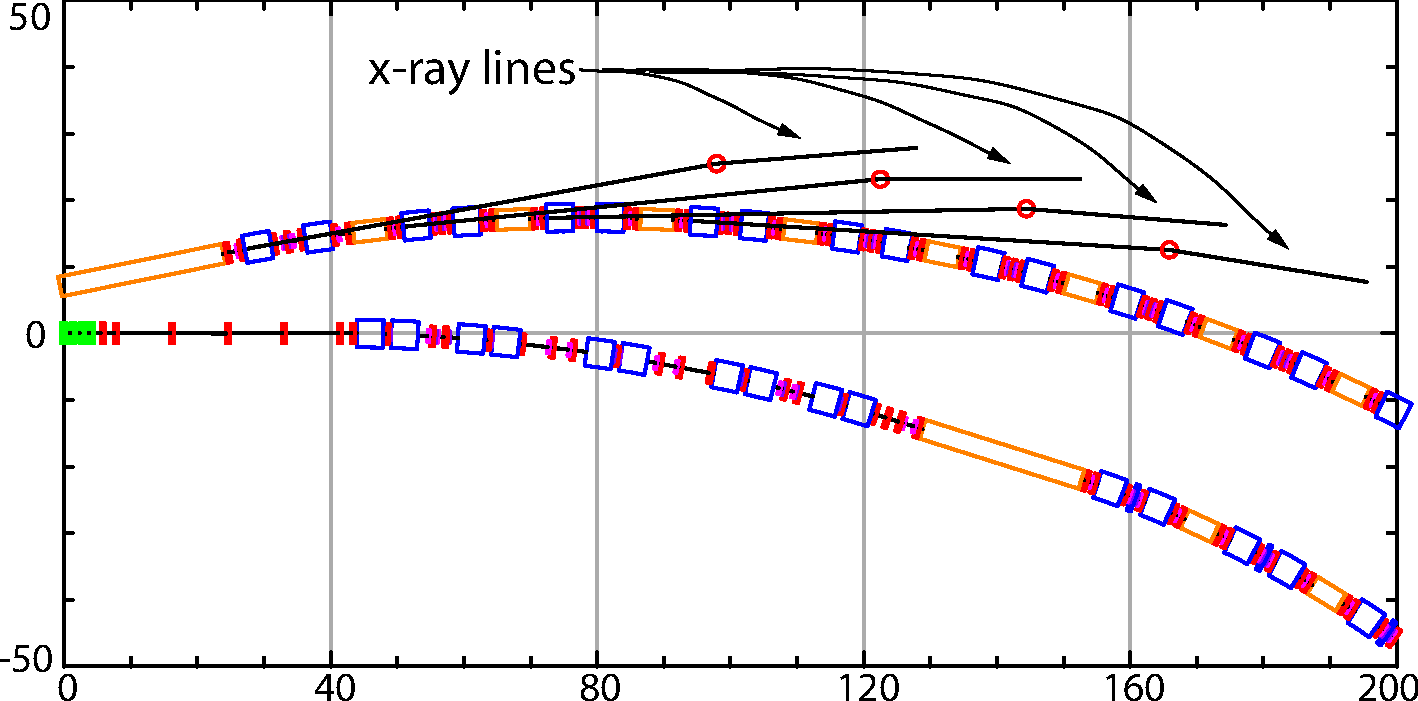
\includegraphics[width=5in]{x-fork.pdf}
  \caption[Example with photon_fork elements.]
  {
Example use of \vn{photon_fork} elements showing four X-ray lines (branches)
attached to a machine.
  }
  \label{f:x.fork}
\end{figure}

A \vn{fork} or \vn{photon_fork} element marks the start of an
alternative \vn{branch} for the beam (or X-rays or other
particles generated by the beam) to follow. 

Collectively \vn{fork} and \vn{photon_fork} elements are called
forking elements. An example geometry is shown in \fig{f:x.fork}.  The
\vn{branch} containing a forking element is called the ``\vn{base}
\vn{branch}''. The \vn{branch} that the forking element points to is
called the ``\vn{target} \vn{branch}''. 

The only difference between \vn{fork} and \vn{photon_fork} is that the
default particle type for the target branch forked from a \vn{fork}
element is the same particle type as the base branch. The default
particle type for the target branch from a \vn{photon_fork} element is
a photon. The actual particle associated with a branch can be set by
setting the \vn{particle} attribute of the forking element.

General \vn{fork} and \vn{photon_fork} attributes are:
\begin{center}
\tt
\begin{tabular}{llll} \toprule
  {\sl Attribute Class}      & Section           & {\sl Attribute Class}      & Section         \\ \midrule
  Aperture limits            & \ref{s:limit}     & Length                     & \ref{s:l}       \\
  Chamber wall               & \ref{s:wall}      & Reference energy           & \ref{s:energy}  \\ 
  Custom Attributes          & \ref{s:cust.att}  & Superposition              & \ref{s:super}   \\
  Description strings        & \ref{s:alias}     & Tracking \& transfer map   & \ref{c:methods} \\ 
  Is_on                      & \ref{s:is.on}     &                            &                 \\
  \bottomrule
\end{tabular}
\end{center}
\toffset
See \sref{s:list.fork} for a full list of element attributes.

Attributes specific to \vn{fork} and \vn{photon_fork} elements are:
\begin{example}
  direction    = <+/- 1>      ! Fork for forward or backwards propagating particles?
  to_line      = <LineName>   ! What line to fork to.
  to_element   = <ElementID>  ! What element to attach to in the line being forked to.
  new_branch   = <T/F>        ! Make a new branch from the to_line? Default = True.
\end{example}

\index{patch}
Branch lines can themselves have forking elements. A branch line
always starts out tangential to the line it is branching from.  A
\vn{patch} element (\sref{s:patch}) can be used to reorient the
reference orbit as needed. Example:
\begin{example}
  from_line: line = (... A, PB, B, ...)  ! Defines base branch
  pb: photon_fork, to_line = x_line
  x_line: line = (X_PATCH, X1, X2, ...)           ! Defines target branch
  x_patch: patch, x_offset = 0.01
  use, from_line
\end{example}
In this example, a photon generated at the fork element \vn{PB} with
$x = 0$ with respect to the \vn{from_line} reference orbit through
\vn{PB} will, when transferred to the \vn{x_line}, and propagated
through \vn{X_PATCH}, have an initial value for $x$ of $-0.01$.

Forking elements have zero length and, like \vn{marker} elements, the
position of a particle tracked through a forking element does not change.

Forking elements do not have orientational attributes like
\vn{x_pitch} and \vn{tilt} (\ref{s:offset}). If the orientation of the
target branch needs to be modified, this can be accomplished using a
\vn{patch} element at the beginning of the line.

\index{is_on}
The \vn{is_on} attribute, while provided for use by a program, is
ignored by \bmad proper.

If the reference orbit needs to be shifted when forking from one ring
to another ring, a patch can be placed in a separate ``transfer'' line
to isolate it from the branches defining the rings. Example:
\begin{example}
  ring1: line = (... A, F1, B, ...)     ! First ring
  x_line: line = (X_F1, X_PATCH, X_F2)  ! ``Transfer'' line
  ring2: line = (... C, F2, D, ...)     ! Second ring
  use, ring1

  f1: fork, to_line = x_line
  f2: fork, to_line = x_line, direction = -1
  x_patch: patch, x_offset = ...
  x_f1: fork, to_line = ring1, to_element = f1, direction = -1
  x_f2: fork, to_line = ring2, to_element = f2
\end{example}
Here the \vn{fork} \vn{F1} in \vn{ring1} forks to \vn{x_line} which
in turn forks to \vn{ring2}.

The above example also illustrates how to connect machines for particles going in the
reverse direction. In this case, \vn{ring2} has a \vn{fork} element \vn{f2} back through
\vn{x_line} and then to \vn{ring1} via the \vn{x_f1} fork. Notice that both \vn{f2} and
\vn{x_f2} have their \vn{direction} attribute set to -1 to indicate that the fork is
appropriate for particles propagating in the -$s$ direction.  Additionally, since \vn{f2}
has \vn{direction} set to -1, it will, by default, connect to the downstream end of the
\vn{x_line}. The default setting of \vn{direction} is 1. 

It is important to note that the setting of \vn{direction} does not change the placement
of elements in the forked line. That is, the global position (\sref{s:global}) of any
element is unaffected by the setting of \vn{direction}. To shift the the global position
of a forked line, \vn{patch} elements must be used.

\index{beginning_ele}\index{fiducial}\index{fork}\index{photon_fork}
\index{marker}\index{to_element}
The \vn{to_element} attribute for a forking element is used to
designate the element of the target branch that the forking element
connects to. To keep things conceptually simple, the \vn{to_element}
must be a ``marker-like'' element which has zero length and unit
transfer matrix. Possible \vn{to_element} types are:
\begin{example}
  beginning_ele
  fiducial
  fork and photon_fork
  marker
\end{example}
When the \vn{to_element} is not specified, the default is to connect
to the beginning of the target branch if \vn{direction} is 1 and to
connect to the end of the target branch if \vn{direction} is -1. In
this case, there is never a problem connecting to the beginning of the
target branch since all branches have a \vn{beginning_ele} element at
the beginning. When connecting to the end of the target branch the
last element in the target branch must be a marker-like element. Note
that, by default, a marker element is placed at the end of all
branches (\sref{s:branch.construct})

The reference energy of a target branch line, needs to be set using
line parameter statements (\sref{s:beginning}). The default reference
particle type of a branch line will be a \vn{photon} is using a
\vn{photon_fork} or will be the same type of particle as the base
branch if a \vn{fork} element is used.

Example showing an injection line branching to a ring which, in turn,
branches to two x-ray lines:
\begin{example}
  inj: line = (..., br_ele, ...)            ! Define the injection line
  use, inj                                  ! Injection line is the root
  br_ele: fork, to_line = ring              ! Fork element to ring
  ring: line = (..., x_br, ..., x_br, ...)  ! Define the ring
  x_br: photon_fork, to_line = x_line       ! Fork element to x-ray line
  x_line: line = (...)                      ! Define the x-ray line
  x_line[E_tot] = 1e3
\end{example}

The \vn{new_branch} attribute is, by default, \vn{True} which means
that the lattice branch created out of the \vn{to_line} line is
distinct from other lattice branches of the same name. Thus, in the
above example, the two lattice branches made from the \vn{x_line} will
be distinct. If \vn{new_branch} is set to \vn{False}, a new lattice
branch will not be created if a lattice branch created from the same
line already exists. This is useful, for example, when a chicane line
branches off from the main line and then branches back to it.

When a lattice is expanded (\sref{s:expand}), the branches defined by
the \vn{use} statement (\sref{s:use}) are searched for fork elements
that branch to new target branches. If found, the appropriate branches are
instantiated and the process repeated until there are no more branches
to be instantiated. This process does {\em not} go in reverse. That is
the lines defined in a lattice file are not searched for fork elements
that have target instantiated branches. For example, if, in the above example,
the use statement was:
\begin{example}
  use, x_line
\end{example}
then only the \vn{x_line} would be instantiated and the lines \vn{inj} and
\vn{ring} would be ignored.

%-----------------------------------------------------------------
\section{Girder}
\label{s:girder}
\index{girder|hyperbf}

\begin{figure}[t]
  \centering
  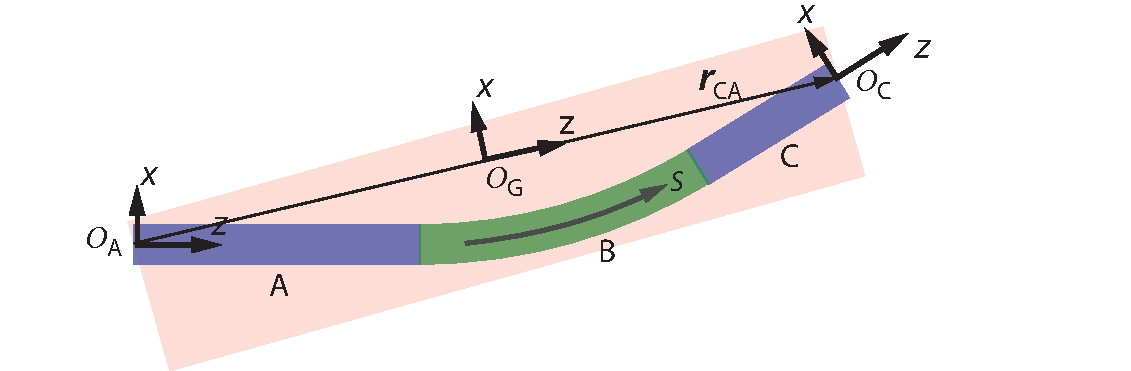
\includegraphics{girder.pdf}
  \caption[Girder example.] {
Girder supporting three elements labeled \vn{A}, \vn{B}, and \vn{C}.
$\calO_A$ is the reference frame at the upstream end of element \vn{A}
(\sref{s:ref.construct}), $\calO_C$ is the reference frame at the
downstream end of element \vn{C}, and $\calO_G$ is the default
\vn{origin} reference frame of the girder. $r_{CA}$ is the vector from
$\calO_A$ to $\calO_C$. The length \vn{l} of the girder is the
difference in $s$ between points $\calO_C$ and $\calO_A$.
  }
  \label{f:girder}
\end{figure}

A \vn{girder} is a support structure that orients the elements that
are attached to it in space. A girder can be used to simulate any
rigid support structure and there are no restrictions on how the lattice
elements that are supported are oriented with respect to one another.
Thus, for example, optical tables can be simulated.

General \vn{girder} attributes are:
\begin{center}
\tt
\begin{tabular}{llll} \toprule
  {\sl Attribute Class}      & Section           & {\sl Attribute Class}      & Section         \\ \midrule
  Custom Attributes          & \ref{s:cust.att}  & Length                     & \ref{s:l}       \\
  Description strings        & \ref{s:alias}     & Offsets, pitches \& tilt   & \ref{s:offset}  \\ 
  Is_on                      & \ref{s:is.on}     &                            &                 \\
  \bottomrule
\end{tabular}
\end{center}
\toffset
See \sref{s:list.girder} for a full list of element attributes.

Attributes specific to a \vn{girder} are:
\index{origin_ele}\index{origin_ele_ref_pt}
\index{x_origin}\index{y_origin}
\index{z_origin}\index{theta_origin}
\index{phi_origin}\index{psi_origin}
Attributes specific to a \vn{floor_shift} elements are:
\begin{example}
  girder = \{<List>\}   ! List of elements on the Girder
  origin_ele        = <Name>     ! Reference element.
  origin_ele_ref_pt = <location> ! Reference pt on reference ele.
  dx_origin         = <Real>     ! x-position offset
  dy_origin         = <Real>     ! y-position offset
  dz_origin         = <Real>     ! z-position offset
  dtheta_origin     = <Real>     ! orientation angle offset.
  dphi_origin       = <Real>     ! orientation angle offset.
  dpsi_origin       = <Real>     ! orientation angle offset.
\end{example}

A simple example of a girder is shown in \fig{f:girder}. Here a girder supports three
elements labeled \vn{A}, \vn{B}, and \vn{C} where \vn{B} is a bend so the geometry is
nonlinear. Such a girder may specified in the lattice file like:
\begin{example}
  g1: girder = \{A, B, C\}
\end{example}

The \vn{girder} statement can take one of two forms:
\begin{example}
  <element_name>: GIRDER = \{<ele1>, <ele2>, ..., <eleN>\}, ... 
\end{example}
or
\begin{example}
  <element_name>: GIRDER = \{<ele_start>:<ele_end>\}, ... 
\end{example}

With the first form, a \vn{girder} element will be created for each section of the lattice where there is a
``consecutive'' sequence of ``slave'' elements \vn{<ele1>} through \vn{<eleN>}.  This
section of the lattice from \vn{<ele1>} through \vn{<eleN>} is called the ``girder support
region''.  ``Consecutive'' here means there are no other elements in the girder support
region except for possibly \vn{drift} and/or \vn{marker} elements.  \vn{Drift} elements
cannot be controlled by a girder but may appear in the girder slave list. If a \vn{drift}
does appear in the slave list, only \vn{marker} elements, but not \vn{dirft} elements will
be ignored when determining if elements are consecutive. Note: If a drift-like element is
desired to be supported by a \vn{girder}, use a \vn{pipe} element instead. \vn{Marker}
elements present in a girder support region, but not mentioned in the girder slave list,
are simply ignored.

The second form of a \vn{girder} statment specifies the first and last elements in the 
sequence of elements to be supported. Everything in between except \vn{drift} elements will
be supported by the \vn{girder}.

Wild card characters (\sref{s:lat.attribs}) can be used in any element
name in the girder slave list. Additionally, beam line names
(\sref{s:lines.wo.arg}) can be used. In this case, any \vn{drift} elements
within a beam line will be ignored.

A lattice element may have at most one \vn{girder} supporting
it. However, a \vn{girder} can be supported by another \vn{girder}
which in turn can be supported by a third \vn{girder}, etc. Girders
that support other girders must be defined in the lattice file after
the supported girders are defined. Example:
\begin{example}
  g1: girder = \{A, B, C\}
  g2: girder = \{g1\}      ! g2 must come after g1!
\end{example}

A \vn{girder} may not directly support \vn{multipass_slave}
(\sref{s:multipass}) or \vn{super_slave} (\sref{s:super})
elements. Rather, a \vn{girder} may support the corresponding lord
elements.

The reference frame from which the girder's offset, pitch, and tilt
attributes (\sref{s:offset}) are measured is constructed as follows: A
reference frame, called the ``\vn{origin}'' reference frame may be
defined using the attributes \vn{origin_ele} and
\vn{origin_ele_ref_pt} which constructs the girder's
\vn{origin} frame to be coincident with the reference frame of another
element. Example:
\begin{example}
  g2: girder = \{...\}, origin_ele = Q, origin_ele_ref_pt = entrance_end
\end{example}
In this example, girder \vn{g2} has an \vn{origin} reference frame
coincident with the entrance end frame of an element named
\vn{Q}. Valid values are
\begin{example}
  entrance_end
  center        ! Default
  exit_end
\end{example}
For \vn{crystal}, \vn{mirror}, and \vn{multilayer_mirror} elements,
setting \vn{origin_ele_ref_pt} to \vn{center} results in the reference
frame being the frame of the surface (cf.~\fig{f:surface}).

If \vn{origin_ele} is not given, the default \vn{origin} frame is
used. The default \vn{origin} frame is constructed as follows:
Let $\calO_A$ be the reference frame of the upstream end of
the first element in the list of supported elements. In this example
it is the upstream end of element \vn{A} as shown in the figure. Let
$\calO_C$ be the downstream end of the last element in the list of
supported elements. In this example this is the downstream end of
element \vn{C}. The origin of the \vn{girder}'s reference frame,
marked $\calO_G$ in the figure, will be half way along the vector
$r_{CA}$ from the origin of $\calO_A$ to the origin of $\calO_B$.  The
orientation of $\calO_G$ is constructed by rotating the $\calO_A$
coordinate system along an axis in $\calO_A$'s $x$-$y$ plane such that
$\calO_A$'s $z$ axis ends up parallel with $r_{CA}$. In the example
above, the rotation axis will be along $\calO_A$'s $y$-axis.

Once the \vn{origin} reference frame is established, the reference
frame of the girder can be offset
from the \vn{origin} frame using the parameters
\begin{example}
  dx_origin    dtheta_origin
  dy_origin    dphi_origin
  dz_origin    dpsi_origin
\end{example} 
The orientation of the \vn{girder}'s reference frame from the \vn{origin}
frame is given in \sref{s:patch.coords}. Example:
\begin{example}
  g3: girder = \{ ... \}, dx_origin = 0.03
\end{example}
This offsets girder \vn{g3}'s reference frame 3~cm horizontally from
the default \vn{origin} frame. If no offsets are given, the
\vn{origin} frame is the same as the girder's reference frame.

The length \vn{l} of a girder, which is not used in any calculations,
is a dependent attribute computed by \bmad and set equal to the $s$
path length between points $\calO_C$ and $\calO_A$.

\index{x_offset}\index{y_offset}\index{x_pitch}\index{y_pitch}\index{tilt}
The physical orientation of the girder with respect to it's reference
frame is, like other elements, determined by the offset, pitch and
tilt orientation attributes as outlined in \sref{s:offset} and
\sref{s:patch.coords}.  When a girder is shifted in space, the elements
it supports are also shifted.  In this case, the orientation
attributes (\vn{x_offset}, \vn{y_pitch}, etc.) give the orientation of
the element with respect to the \vn{girder}. The orientation with
respect to the local reference coordinates is given by
\vn{x_offset_tot}, which are computed from the orientation attributes
of the element and the \vn{girder}. An example will make this clear:
\begin{example}
  q1: quad, l = 2
  q2: quad, l = 4, x_offset = 0.02, x_pitch = 0.01
  d: drift, l = 8
  g4: girder = \{q1, q2\}, x_pitch = 0.002, x_offset = 0.03
  this_line: line = (q1, d, q2)
  use, this_line
\end{example}
\index{overlay}
In this example, \vn{g4} supports quadrupoles \vn{q1} and \vn{q2}.
Since the supported elements are colinear, the computation is greatly
simplified. The reference frame of \vn{g4}, which is the default
\vn{origin} frame, is at $s = 7$~meters which is half way between the
start of \vn{q1} at at $s = 0$~meters and the end of \vn{q2}) which is
at $s = 14$. The reference frames of \vn{q1} and \vn{q2} are at their
centers so the $s$ positions of the reference frames is
\begin{example}
  Element        S_ref   dS_from_g4
  q1             1.0     -6.0
  g4             7.0      0.0
  q2            12.0      5.0
\end{example}
Using a small angle approximation to simplify the calculation, the
\vn{x_pitch} of \vn{g4} produces an offset at the center of \vn{q2} of
$0.01 = 0.002 * 5$. This, added to the offsets of \vn{g4} and \vn{q2},
give the total offset of \vn{q2} to be $0.06 = 0.01 + 0.03 + 0.02$.
The total \vn{x_pitch} of \vn{q2} is $0.022 = 0.02 + 0.001$.

A \vn{girder} that has its \vn{is_on} attribute set to False is considered to be
unsifted with respect to it's reference frame.

%-----------------------------------------------------------------------------
\section{Group}
\label{s:group}
\index{group|hyperbf}

\vn{Group} elements are a type of \vn{control} element
(\sref{s:lord.slave}) used to make variations in the attributes of
other elements (called ``slave'' attributes) during execution of a
program. For example, to simulate the action of a control room knob
that changes the beam tune in a storage ring, a \vn{group} element can
be used to vary the strength of selected quads in a specified
manner. Also see \vn{overlay} (\sref{s:overlay}) The difference
between \vn{group} and \vn{overlay} elements is that \vn{overlay}
elements set the values of the attributes directly while \vn{group}
elements make delta changes to attribute values.

General \vn{girder} attributes are:
\begin{center}
\tt
\begin{tabular}{llll} \toprule
  {\sl Attribute Class}      & Section           & {\sl Attribute Class}      & Section         \\ \midrule
  Custom Attributes          & \ref{s:cust.att}  & Description strings        & \ref{s:alias}   \\ 
  \bottomrule
\end{tabular}
\end{center}
\toffset
See \sref{s:list.group} for a full list of element attributes.

\index{var}
Attributes specific to a \vn{Group} element are:
\begin{example}
  var = \{<var1>, <var2>, ...\}   ! List of variables.
\end{example}

The general syntax for a \vn{group} element is
\begin{example}
  name: GROUP = \{ele1[attrib1]:exp1, ele2[attrib2]:exp2, ...\}, 
                 VAR = \{var1, var2, ...\}, var1 = init_val1, ...
\end{example}
\textbf{See Section~\sref{s:go.syntax} for a detailed description of this syntax.}

As explained further below, there are two numbers associated with each
variable in a group: One number is the value of the variable (also
called the ``present'' value) and the other number is the ``old''
value. To refer to these old values prepend the string ``old_'' to the
variable name. Thus, in the above example, the old variable values
have names \vn{old_a} and \vn{old_b} and these old values can be set
in the same manner as the present values. Example:
\begin{example}
  gr1: group = \{...\}, var = \{a, b\}, old_a = 1
  gr2[old_b] = 2
\end{example}

A \vn{group} element is like an \vn{overlay} element in that a
\vn{group} element controls the attribute values of other ``slave''
elements. Unlike an \vn{overlay}, which sets a specific value directly,
a \vn{group} element is used to make changes in value. An
example will make this clear:
\begin{example}
  gr: group = \{q1[k1]:a^2\}, var = \{a\} 
  q, quad, k1 = 0.5
\end{example}
When a program reads the lattice, the value of \vn{q[k1]} will be 0.5
and the value of \vn{gr[a]}, along with the associated old value
\vn{gr[old_a]} will have the default value of 0. Now if the program
sets \vn{gr[a]} (just as a program can set any attribute in the
lattice) to, say, the value 0.3, the \bmad bookkeeping code will
compute a delta value of
\begin{example}
  delta = a^2 - old_a^2
        = 0.09
\end{example}
In general, deltas are computed as the difference between the
arithmetic expression evaluated with the present variable values and
the arithmetic expression evaluated with the old variable values. In
the present example, there is a single delta and it is applied to
\vn{q[k1]} which gives this attribute a value of 0.59 = 0.5 +
0.09. After all deltas are applied, the old variable values are set to
the present variable values so that further evaluations will give zero
deltas. In the present example, \vn{gr[old_a]} is set to 0.3 which is
the value of \vn{gr[a]}

Within a program, if both a group variable and a slave attribute are
modified, the value of the slave attribute will be dependent upon the
order of which is modified first. For example:
\begin{example}
  gr: group = \{q[k1]:a^2\}, var = \{a\} 
  q, quad
\end{example}
Now if a program first sets \vn{gr[a]} to 0.3 and then sets \vn{q[k1]}
to 0.5, the result is that \vn{q[k1]} will have a value of 0.5. That
is, the value of \vn{q[k1]} will be independent of \vn{gr[a]}. If the
setting is reversed so that \vn{q[k1]} is set first, the value of
\vn{q[k1]} will be 0.59. Since the result is order dependent, trying
to ``simultaneously'' vary the attributes of both group variables and
slave attributes can lead to unpredictable results. For example,
consider lattice ``optimization'' where a program varies a set of
lattice parameters to achieve certain goals (for example, minimum beta
at some point in the lattice, etc.). If the list of parameters to be
varied contains both group variables and slave attributes, the actual
changes to slave attributes may be different from what the program
expects when the program varies its list of parameters.

When a lattice file is read in, variable values for any groups are
always applied last. This is independent of the order that they appear
in the file. For example:
\begin{example}
  gr: group = \{q1[k1]:a^2\}, var = \{a\}, a = 0.6, old_a = 0.2
  q, quad, k1 = 0.5
\end{example}
In this example, when the lattice is read in, the value of q1[k1] would be
$0.57 = 0.5 + (0.6^2 - 0.2^2)$ 

\index{overlay}\index{girder}
Different \vn{group} elements may control the same slave attribute and
a \vn{group} element may control other \vn{group}, \vn{overlay} or
\vn{girder} element attributes. However, It does not make sense, and
it is not permitted, for a \vn{group} element to control the same
attribute as an \vn{overlay} element or for a \vn{group} element to
control a \vn{dependent} attribute (\sref{s:depend}). To setup a group
element to control the same slave attribute as an \vn{overlay}, define
an intermediate \vn{overlay}. For example:
\begin{example}
  ov: overlay = \{q{k1}\, q2[k1], ...\}, var = \{a\}
  q, quad                                          
  gr: group = \{ov_q[k1]:a^2\}, var = \{a\}  ! New
  ov_q: overlay = \{q\}, var = \{k1\}        ! New
\end{example}
In this example, the overlay \vn{ov} controls the attribute \vn{q[k1]}
so it is not permitted for \vn{q[k1]} to be a slave of a group
element.  To have group control of \vn{q[k1]}, two elements are
introduced: the group \vn{gr} is setup controlling \vn{ov_q[k1]} and
overlay \vn{ov_q} is an overlay that controls \vn{q[k1]}. Notice that
trying to control \vn{ov} directly by a group element will not work
since \vn{ov} controls multiple elements.

\index{accordion_edge}\index{start_edge}
\index{end_edge}\index{symmetric_edge}
\index{z_offset}
A \vn{group} can be used to control an elements position and length
using one of the following attributes:
\begin{example}
  accordion_edge  ! Element grows or shrinks symmetrically
  start_edge      ! Varies element's upstream edge s-position
  end_edge        ! Varies element's downstream edge s-position
  s_position      ! Varies element's overall s-position. Constant length.
\end{example}
With \vn{accordion_edge}, \vn{start_edge}, \vn{end_edge}, and
\vn{symmetric_edge} the longitudinal position of an elements edges are
varied. This is done by appropriate control of the element's length
and the lengths of the elements to either side. With \vn{s_position}
the physical element is offset from its reference position
(\sref{s:offset}) and the elements on either side are untouched.  In
all cases the total length of the lattice is kept invariant.

As an example, consider \vn{accordion_edge} which varies the edges of
an element so that the center of the element is fixed but the length
varies':
\begin{example}
  gr: group = \{Z[accordion_edge]\}, var = \{offset\}
\end{example}
A change of, say, 0.1 \vn{gr}'s \vn{offset} variable moves both edges
of element \vn{Z} by 0.1 meters so that the length of \vn{Z} changes
by 0.2 meters but the center of \vn{Z} is constant. To keep the total
lattice length invariant, the lengths of the elements to either side
are decreased by 0.1 meters to keep the total lattice length constant.
\begin{example}
  q10: quad, l = ...
  q11: quad, l = ...
  d1: drift, l = ...
  d2: drift, l = ...
  this_line: line = (... d1, q10, d2, q11, ...)
  gr2: group = \{q10[start_edge]\}, var = \{a\}, a = 0.1
\end{example}
The effect of  \vn{gr2[a]} will be to lengthen the length of
\vn{q10} and shorten the length of \vn{d1}.

A lattice file may contain lines and lattice elements that are not
part of the actual lattice when the lattice is constructed. \vn{Group}
elements where {\em none} of its slave elements are part of the
finished lattice are ignored and are also not part of the finished
lattice. It is not permitted to have \vn{group} elements that have
some slave elements that are part of the finished lattice and some
slave elements that are not.

If the arithemtical expression used for an \vn{group} contains an element attribute,
care must be taken if that element attribute is changed. This is discussed in
\sref{s:arith} and \sref{s:go.syntax}.

%-----------------------------------------------------------------
\section{Hybrid}
\label{s:hybrid}
\index{hybrid|hyperbf}

A \vn{hybrid} element is an element that is formed by concatenating
other element together. \vn{hybrid} elements are not part of the input
lattice file but are created by a program, usually for speed purposes.

%-----------------------------------------------------------------
\section{Instrument, Monitor, and Pipe}
\label{s:monitor}
\index{instrument|hyperbf}
\index{monitor|hyperbf}
\index{pipe|hyperbf}

Essentially \bmad treats \vn{instrument}, \vn{monitor}, and \vn{pipe}
elements like a \vn{drift}. There is a difference, however, when
superimposing elements (\sref{s:super}). For example, a
\vn{quadrupole} superimposed on top of a \vn{drift} results in a free
\vn{quadrupole} element in the tracking part of the lattice and no
lord elements are created. On the other hand, a \vn{quadrupole}
superimposed on top of a \vn{monitor} results in a \vn{quadrupole}
element in the tracking part of the lattice and this \vn{quadrupole}
element will have two lords: A \vn{quadrupole} superposition lord and
a \vn{monitor} superposition lord.

General \vn{instrument}, \vn{monitor}, and \vn{pipe} attributes are:
\begin{center}
\tt
\begin{tabular}{llll} \toprule
  {\sl Attribute Class}      & Section             & {\sl Attribute Class}      & Section          \\ \midrule
  Aperture limits            & \ref{s:limit}       & Length                     & \ref{s:l}       \\
  Chamber wall               & \ref{s:wall}        & Offsets, pitches \& tilt   & \ref{s:offset}  \\ 
  Custom Attributes          & \ref{s:cust.att}    & Reference energy           & \ref{s:energy}  \\
  Description strings        & \ref{s:alias}       & Superposition              & \ref{s:super}   \\
  Hkick \& Vkick             & \ref{s:kick}        & Symplectify                & \ref{s:symp}    \\
  Instrumental variables     & \ref{s:meas.attrib} & Tracking \& transfer map   & \ref{c:methods} \\
  Is_on                      & \ref{s:is.on}       &                            &                 \\
  \bottomrule
\end{tabular}
\end{center}
\toffset
See \sref{s:list.instrument} for a full list of element attributes.

\index{x_offset}
\index{y_offset}
\index{x_pitch}
\index{y_pitch}
\index{tilt}
The \vn{offset}, \vn{pitch}, and \vn{tilt} attributes are not
used by any \bmad routines. If these attributes are used by a program
they are typically used to simulate such things as measurement
offsets. The \vn{is_on} attribute is also not used by \bmad
proper. Example:
\begin{example}
  d21: instrum, l = 4.5
\end{example}

%-----------------------------------------------------------------
\section{Kickers: Hkicker and Vkicker}
\label{s:hvkicker}
\index{hkicker|hyperbf}
\index{vkicker|hyperbf}

An \vn{hkicker} gives a beam a horizontal kick and a \vn{vkicker} gives a 
beam a vertical kick. Also see the \vn{kicker} (\sref{s:kicker}) element.

General \vn{hkicker} \vn{vkicker} attributes are:
\begin{center}
\tt
\begin{tabular}{llll} \toprule
  {\sl Attribute Class}      & Section           & {\sl Attribute Class}      & Section         \\ \midrule
  Aperture limits            & \ref{s:limit}     & Length                     & \ref{s:l}       \\
  Chamber wall               & \ref{s:wall}      & Mag \& Elec multipoles     & \ref{s:multip}  \\
  Custom Attributes          & \ref{s:cust.att}  & Offsets, pitches \& tilt   & \ref{s:offset}  \\
  Description strings        & \ref{s:alias}     & Reference energy           & \ref{s:energy}  \\ 
  Field Maps                 & \ref{s:fieldmap}  & Superposition              & \ref{s:super}   \\
  Fringe Fields              & \ref{s:fringe}    & Symplectify                & \ref{s:symp}    \\
  Hkick \& Vkick             & \ref{s:kick}      & Tracking \& transfer map   & \ref{c:methods} \\
  Is_on                      & \ref{s:is.on}     &                            &                 \\
  \bottomrule
\end{tabular}
\end{center}
\toffset
See \sref{s:list.hvkicker} for a full list of element attributes.

\index{kick}
\index{hkick}
\index{vkick}
Note that \vn{hkicker} and \vn{vkicker} elements use the
\vn{kick} attribute while a \vn{kicker} uses the \vn{hkick} and \vn{vkick} 
attributes. Example:
\begin{example}
  h_kick: hkicker, l = 4.5, kick = 0.003
\end{example}

%-----------------------------------------------------------------
\section{Kicker}
\label{s:kicker}
\index{kicker|hyperbf}

\index{hkick}\index{vkick}
\index{h_displace}\index{v_displace}
A \vn{kicker} can deflect a beam in both planes. Note that a
\vn{kicker} uses the \vn{hkick} and \vn{vkick} attributes while
\vn{hkicker} and \vn{vkicker} elements use the \vn{kick} attribute. 
In addition, a \vn{kicker} can apply a displacement to a particle
using the \vn{h_displace} and \vn{v_displace} attributes.

General \vn{kicker} attributes are:
\begin{center}
\tt
\begin{tabular}{llll} \toprule
  {\sl Attribute Class}      & Section           & {\sl Attribute Class}      & Section          \\ \midrule
  Mag \& Elec multipoles     & \ref{s:multip}    & Length                     & \ref{s:l}        \\
  Aperture limits            & \ref{s:limit}     & Offsets, pitches \& tilt   & \ref{s:offset}   \\
  Chamber wall               & \ref{s:wall}      & Overlapping Fields         & \ref{s:overlap}  \\
  Custom Attributes          & \ref{s:cust.att}  & Reference energy           & \ref{s:energy}   \\ 
  Description strings        & \ref{s:alias}     & Superposition              & \ref{s:super}    \\
  Fringe Fields              & \ref{s:fringe}    & Symplectify                & \ref{s:symp}     \\
  Hkick \& Vkick             & \ref{s:kick}      & Field Maps                 & \ref{s:fieldmap} \\
  Is_on                      & \ref{s:is.on}     & Tracking \& transfer map   & \ref{c:methods}  \\ 
  \bottomrule
\end{tabular}
\end{center}
\toffset
See \sref{s:list.kicker} for a full list of element attributes.

Example:
\begin{example}
  a_kick: kicker, l = 4.5, hkick = 0.003
\end{example}

%-----------------------------------------------------------------
\section{Lcavity}
\label{s:lcav}
\index{lcavity|hyperbf}

An \vn{lcavity} is a LINAC accelerating cavity.  The main difference between an
\vn{rfcavity} and an \vn{lcavity} is that, unlike an \vn{rfcavity}, the reference energy
(\sref{s:phase.space}) through an \vn{lcavity} is not constant.

General \vn{lcavity} attributes are:
\begin{center}
\tt
\begin{tabular}{llll} \toprule
  {\sl Attribute Class}      & Section           & {\sl Attribute Class}      & Section            \\ \midrule
  Aperture limits            & \ref{s:limit}     & Offsets, pitches \& tilt   & \ref{s:offset}     \\
  Chamber wall               & \ref{s:wall}      & Overlapping Fields         & \ref{s:overlap}    \\
  Custom Attributes          & \ref{s:cust.att}  & Reference energy           & \ref{s:energy}     \\ 
  Description strings        & \ref{s:alias}     & RF Couplers                & \ref{s:rf.coupler} \\
  Field autoscaling          & \ref{s:autoscale} & Superposition              & \ref{s:super}      \\
  Fringe Fields              & \ref{s:fringe}    & Symplectify                & \ref{s:symp}       \\
  Hkick \& Vkick             & \ref{s:kick}      & Field Maps                 & \ref{s:fieldmap}   \\
  Is_on                      & \ref{s:is.on}     & Tracking \& transfer map   & \ref{c:methods}    \\
  Length                     & \ref{s:l}         & Wakes                      & \ref{s:wakes}      \\
  \bottomrule
\end{tabular}
\end{center}
\toffset
See \sref{s:list.lcavity} for a full list of element attributes.

The attributes specific to an \vn{lcavity} are 
\index{gradient}\index{phi0}\index{n_cell}
\index{phi0_multipass}\index{e_loss}
\index{rf_frequency}\index{voltage}\index{cavity_type}
\begin{example}
  cavity_type     = <Switch>  ! Type of cavity.
  gradient        = <Real>    ! Accelerating gradient (V/m).
  gradient_err    = <Real>    ! Accelerating gradient error (V/m).
  phi0            = <Real>    ! Phase (rad/2\(\pi\)) of the reference particle with 
                              !   respect to the RF. phi0 = 0 is on crest.
  phi0_multipass  = <Real>    ! Phase with respect to a multipass lord (rad/2\(\pi\)).
  phi0_err        = <Real>    ! Phase error (rad/2\(\pi\))
  e_loss          = <Real>    ! Loss parameter for short range wake fields (V/Coul).
  rf_frequency    = <Real>    ! Rf frequency (Hz).
  voltage                     ! Cavity voltage. Dependent attribute (\sref{s:depend}).
  n_cell          = <Integer> ! Number of cavity cells. Default is 1.
\end{example}

The dependent variable \vn{voltage} attribute can be used in place of
\vn{gradient} as discussed in \sref{s:depend}.  \vn{voltage} is a
dependent attribute and is defined to be
\begin{example}
  voltage = gradient * L
\end{example}

The energy kick felt by a particle, assuming no phase slippage, is 
\begin{example}
  dE = gradient_tot * L * cos(\(2\,\pi\) * (\(\phi_\text{particle}\) + \(\phi_\text{ref}\)))
\end{example}
\index{multipass}
where the total gradient is
\begin{example}
  gradient_tot = (gradient + gradient_err) * field_autoscale
\end{example}
The phase $\phi_{\text{ref}}$ is
\begin{example}
  \(\phi_{\text{ref}}\) = phi0 + phi0_multipass + phi0_err + phi0_autoscale
\end{example}
and $\phi_t$ is the part of the phase due to when the particle arrives
at the cavity and depends upon whether \vn{absolute time tracking} or 
\vn{relative time tracking} as discussed in \sref{s:rf.time}.

\vn{phi0_multipass} is only to be used to shift the phase with respect to a
\vn{multipass} lord. See \sref{s:multipass}.

\vn{phi0_autoscale} and \vn{field_autoscale} are calculated by \bmad's auto-scale
module. See Section~\sref{s:autoscale} for more details. Autoscaling can be toggled on/off
by using the \vn{autoscale_phase} and \vn{autoscale_amplitude} toggles.

The energy change of the reference particle is just the energy change for a 
particle with $z = 0$ and no phase or gradient errors. Thus
\begin{example}
  dE(reference) = gradient * L * cos(\(2\,\pi\) * \(\phi_{\text{ref}}\))
\end{example}

The energy kick for a \bmad \vn{lcavity} is consistent with MAD. 
Note: The MAD8 documentation for an \vn{lcavity} has a wrong
sign. Essentially the MAD8 documentation gives
\begin{example}
  dE = gradient * L * cos(\(2\,\pi\) * (\(\phi_{\text{ref}}\) - phi(z))) ! WRONG
\end{example}
This is incorrect. 

When short-range wake fields are being simulated, with
\vn{bmad_com%sr_wakes_on = True} (\sref{s:bmad.com}), the
\vn{e_loss} attribute can be used to modify the gradient in order to
maintain a constant average energy gain. That is, \vn{e_loss} can be
used to simulate the effect of a feedback circuit that attempts to
maintain the average energy of the bunch after the element constant.
The energy kick is then
\begin{example}
  dE(with wake) = dE + e_loss * n_part * e_charge 
\end{example}
\vn{n_part} is set using the \vn{parameter} statement (\sref{s:param})
and represents the number of particles in a bunch. \vn{e_charge} is
the charge on an electron (Table~\ref{t:constants}). Notice that the
\vn{e_loss} term is independent of the sign of the charge of the particle.

The \vn{cavity_type} is the type of cavity being simulated. Possible
settings are:
\begin{example}
  ptc_standard
  standing_wave    ! Default
  traveling_wave
\end{example}
The \vn{cavity_type} switch is ignored if a field map is used.
With the \vn{standing_wave} setting, the transverse trajectory through
an \vn{lcavity} is modeled using equations developed by Rosenzweig and
Serafini\cite{b:rosenzweig} modified to give the correct phase-space
area at non ultra-relativistic energies.  See Section
\sref{s:lcavity.std} for more details.  Note: The transfer matrix for
an \vn{lcavity} with finite \vn{gradient} is never symplectic. See
\sref{s:phase.space}. In addition, couplers (\sref{s:rf.coupler}) and
HOM wakes (\sref{s:wakes}) can be modeled.

When using \vn{boris} or \vn{runge_kutta}, tracking (\sref{s:tkm})
through a field map (\sref{s:fieldmap}), the \vn{bmad_standard} field
is \vn{n_cell} half wave resonators.

Example:
\begin{example}
  lwf: lcavity, l = 2.3, rf_frequency = 500e6, voltage = 20e6
\end{example}

{\em Note: The default \vn{bmad_standard} tracking for \vn{lcavity}
elements when the velocity $\beta$ is significantly different from 1
can only be considered as a rough approximation. Indeed, the only
accurate way to simulate a cavity in this situation is by integrating
through the actual field [Cf.~Runge Kutta tracking (\sref{s:tkm})]}

%-----------------------------------------------------------------
\section{Marker}
\label{s:mark}
\index{marker|hyperbf}

A \vn{marker} is a zero length element meant to mark a position. 

General \vn{marker} attributes are:
\begin{center} 
\tt
\begin{tabular}{llll} \toprule
  {\sl Attribute Class}      & Section             & {\sl Attribute Class}        & Section         \\ \midrule
  Aperture limits            & \ref{s:limit}       &   Is_on                      & \ref{s:is.on}   \\ 
  Chamber wall               & \ref{s:wall}        & Offsets \& tilt              & \ref{s:offset}  \\
  Custom Attributes          & \ref{s:cust.att}    & Reference energy             & \ref{s:energy}  \\
  Description strings        & \ref{s:alias}       & Superposition                & \ref{s:super}   \\
  Instrumental variables     & \ref{s:meas.attrib} & Tracking \& transfer map     & \ref{c:methods} \\ 
  \bottomrule
\end{tabular}
\end{center}
\toffset
See \sref{s:list.marker} for a full list of element attributes.

\index{x_ray_line_len}
Attributes specific to a \vn{marker} element are:
\begin{example}
  x_ray_line_len = <Real>
\end{example}

\vn{x_ray_line_len} is the length of an associated x-ray synchrotron
light line measured from the marker element. This is used for
machine geometry calculations and is irrelevant for lattice
computations.

\index{x_offset}\index{y_offset}
\index{tilt}\index{is_on}
The \vn{x_offset}, \vn{y_offset} and \vn{tilt} attributes are not used
by any \bmad routines. Typically, if these attributes are used by a
program, they are used to simulate things like BPM offsets. The
\vn{is_on} attribute is also not used by \bmad proper. 

Example:
\begin{example}
  mm: mark, type = "BPM"
\end{example}

%-----------------------------------------------------------------
\section{Mask}
\label{s:mask}
\index{mask|hyperbf}

A \vn{mask} element defines an aperture where the mask area can
essentially have an arbitrary shape. 

For X-ray tracking, a \vn{mask} element is similar to a
\vn{diffraction_plate} (\sref{s:diff.plate}) element except that with
a \vn{diffraction_plate} element, coherent effects are taken into
account while, with a \vn{mask} element, coherent effects are ignored.
Also a \vn{mask} element can be used with charged particles while a
\vn{diffraction_plate} cannot.

General \vn{mask} element attributes are:
\begin{center}
\tt 
\begin{tabular}{llll} \toprule
  {\sl Attribute Class}      & Section           & {\sl Attribute Class}      & Section         \\ \midrule
  Aperture limits            & \ref{s:limit}     & Offsets, pitches \& tilt   & \ref{s:offset}  \\
  Custom Attributes          & \ref{s:cust.att}  & Reference energy           & \ref{s:energy}  \\
  Description strings        & \ref{s:alias}     & Superposition              & \ref{s:super}   \\
  Is_on                      & \ref{s:is.on}     & Tracking \& transfer map   & \ref{c:methods} \\
  Mask geometry              & \ref{s:wall}      &                            &                 \\ 
  \bottomrule
\end{tabular}
\end{center}
\toffset
See \sref{s:list.mask} for a full list of element attributes.

Notice that, unlike a \vn{rcollimator} or a \vn{ecollimator}, a \vn{mask} element has zero length.

\index{mode}\index{field_scale_factor}
Attributes specific to a \vn{mask} element are:
\begin{example}
  mode               = <Type>   ! Reflection or transmission.
  field_scale_factor = <Real>   ! Factor to scale the photon field
  ref_wavelength                ! Reference wavelength (\sref{s:energy}). Dependent attribute (\sref{s:depend}).
\end{example}

Note: These attributes are only pertinent for photon tracking. Charged
particle tracking assumes transmission mode and does not use
\vn{field_scale_factor} and \vn{ref_wavelength} attributes.

The \vn{mode} switch, which is only used for photon tracking, sets
whether X-rays are transmitted through the \vn{mask} or
or reflected. Possible values for the \vn{mode} switch are:
\begin{example}
  reflection
  transmission        ! Default
\end{example}

The geometry of the mask, that is, where the openings (in
transmission mode) or reflection regions are, is defined using the
``wall'' attribute. See (\sref{s:wall}) for more details.

In transmission mode, a \vn{mask} is nominally orientated
transversely to the beam. Like all other elements, the
\vn{mask} can be reoriented using the element's offsets,
pitches and tilt attributes (\sref{s:offset}).

\index{aperture_type}
The \vn{aperture_type} (\sref{s:limit}) parameter of a
\vn{mask} will default to \vn{auto} which will set the
aperture limits to define a rectangular aperture that just cover the
clear area of the mask.

\index{field_scale_factor}
The \vn{field_scale_factor}, if set to a non-zero value (zero is the
default) will be used to scale the field of photons as they pass through
the \vn{mask} element:
\begin{example}
  field -> field * field_scale_factor
\end{example}
Scaling is useful since the electric field of photons traveling through a
\vn{mask} are renormalized (see \Eqs{eeo4p} and
\eq{eek4p}). This can lead to large variation of the photon field and
can, for example, make visual interpretation of plots of field verses
longitudinal position difficult to interpret. \vn{field_scale_factor}
can be used to keep the field more or less constant.

A \vn{mask} that is ``turned off'' (\vn{is_on} attribute set to
False), does not mask at all and transmits everything.

Example:
\begin{example}
  scrapper: mask, wall = \{...\}
\end{example}

%-----------------------------------------------------------------
\section{Match}
\label{s:match}
\index{match|hyperbf}

A \vn{match} element is used to match the Twiss parameters between two
points. 

General \vn{match} attributes are:
\begin{center} 
\tt
\begin{tabular}{llll} \toprule
  {\sl Attribute Class}      & Section           & {\sl Attribute Class}      & Section         \\ \midrule
  Aperture limits            & \ref{s:limit}     & Length                     & \ref{s:l}       \\
  Custom Attributes          & \ref{s:cust.att}  & Reference energy           & \ref{s:energy}  \\ 
  Description strings        & \ref{s:alias}     & Superposition              & \ref{s:super}   \\ 
  Is_on                      & \ref{s:is.on}     &                            &                 \\
  \bottomrule
\end{tabular}
\end{center}
\toffset
See \sref{s:list.match} for a full list of element attributes.

Attributes specific to a \vn{match} element are:
\begin{example}
  beta_a0   = <Real>,  beta_b0  = <Real>   ! Beginning betas
  beta_a1   = <Real>,  beta_b1  = <Real>   ! Ending betas
  alpha_a0  = <Real>,  alpha_b0 = <Real>   ! Beginning alphas
  alpha_a1  = <Real>,  alpha_b1 = <Real>   ! Ending alphas
  eta_x0    = <Real>,  eta_y0   = <Real>   ! Beginning etas 
  eta_x1    = <Real>,  eta_y1   = <Real>   ! Ending etas 
  etap_x0   = <Real>,  etap_y0  = <Real>   ! Beginning eta' 
  etap_x1   = <Real>,  etap_y1  = <Real>   ! Ending eta'
  dphi_a    = <Real>,  dphi_b   = <Real>   ! Phase advances
  match_end = <Logic>                      ! See below. Default is False.
  x0, px0, y0, py0, z0, pz0 = <Real>       ! Beginning coordinates
  x1, px1, y1, py1, z1, pz1 = <Real>       ! Ending coordinates
  match_end_orbit = <Logic>                ! See below. Default is False.
\end{example}

The transfer map for a \vn{match} element is a linear transformation 
with a ``kick'':
\Begineq
  r_1 = \Bf M \, r_0 + \Bf V 
\Endeq
where $r_1$ is the output coordinates, and $r_0$ are the input
coordinates. The matrix $\Bf M$ is the linear part of the map and the
vector $\Bf V$ is the zeroth order part of the map.

\index{beta_a0}\index{beta_b0}
\index{beta_a1}\index{beta_b1}
\index{eta_x0}\index{etap_x0}
\index{eta_y0}\index{etap_y0}
\index{dphi_a}\index{dphi_b}
Nomenclature: The parameters \vn{beta_a0}, \vn{alpha_a0}, etc. of the
\vn{match} element are called the beginning (upstream) ``design''
Twiss parameters. The parameters \vn{beta_a1}, \vn{alpha_a1}, etc. of
the \vn{match} element are called the ending (downstream) ``design'' Twiss
parameters.

The matrix $\Bf M$ is calculated such that if (and only if) the actual
(computed) Twiss parameters at the beginning \vn{match} element are
equal to the beginning design Twiss parameters, then the computed
Twiss parameters at the end of the \vn{match} element will be the end
design Twiss parameters and the phase advances (in radians) will be
\vn{dphi_a} and \vn{dphi_b}.

\index{x0}\index{px0}\index{y0}\index{py0}\index{z0}\index{pz0}
\index{x1}\index{px1}\index{y1}\index{py1}\index{z1}\index{pz1}
The kick term $\Bf V$ is constructed so that if a particle has
coordinates \vn{(x0, px0, y0, py0, z0, pz0)} before the \vn{match}
element, the coordinates just after the element will be \vn{(x1, px1,
y1, py1, z1, pz1)}. With this, $\Bf V$ will be:
\Begineq
  \Bf V = 
    \begin{pmatrix} 
    \text{x1} \\ \text{px1} \\ \text{y1} \\ \text{py1} \\ \text{z1} \\ \text{pz1} 
    \end{pmatrix} -
    \Bf M \, \begin{pmatrix} 
    \text{x0} \\ \text{px0} \\ \text{y0} \\ \text{py0} \\ \text{z0} \\ \text{pz0} 
    \end{pmatrix}
\Endeq

\index{l}
The length attribute \vn{l} is not used in the transfer matrix
calculation. The length \vn{l} is used to compute the time it takes to
go through a match element.

Example:
\begin{example}
  mm: match, beta_a0 = 12.5, beta_b0 = 3.4, eta_x0 = 1.0, ...
\end{example}

  \begin{description} 
  \index{open}
  \index{match_end}\index{match_end_input}
  \item[match_end, match_end_input] \Newline
The default value of \vn{match_end} is False. The \vn{match_end}
attribute is used for appropriately setting the beginning design Twiss
parameters from within a program. If the \vn{match_end} attribute is
set to True, the beginning design Twiss parameters are set to be equal
to the actual Twiss parameters from the exit end of the previous
element. In this case, the actual Twiss parameters at the end of the
match element will be the design end Twiss parameters. The
\vn{match_end} attribute may only be set to True with \vn{open}
lattices (\sref{s:param}) since, for a \vn{closed} lattice, it is not
possible to calculate the Twiss parameters at the previous element
independently of the design end Twiss parameters at the \vn{match}
element.

When running a program, if a \vn{match} element initially has it's
\vn{match_end} attribute is set to True, the \bmad bookkeeping
routines will ensure that the \vn{match} element's beginning design
Twiss parameters are appropriately set as explained above. If
\vn{match_end} is now toggled to False by the program, the beginning
Twiss attribute values, and hence the transfer matrix for the
\vn{match} element, will be frozen. Thereafter, variation of any
parameter in the lattice that affects the calculated Twiss parameters
through the \vn{match} element will not affect the \vn{match}
element's transfer matrix.

When a lattice is read in, the \vn{match_end_input} attribute is set by \bmad to be equal
to \vn{match_end}. This attribute is not settable by the user and is simply present to
tell the user what the setting of \vn{match_end} was in the lattice file.

  \index{match_end_orbit}\index{match_end_orbit_input}
  \item[match_end_orbit, match-end_orbit_input]
The \vn{match_end_orbit} attribute is similar in operation to the \vn{match_end}
attribute. The default value of \vn{match_end_orbit} is False. When
running a program, if \vn{match_end_orbit} is set to True, when any
particle is tracked through the \vn{match} element, the \vn{match}
element's starting coordinate parameters, \vn{(x0, px0, y0, py0, z0,
pz0)}, will be set to the particle's coordinates at the exit end of
the previous element. That is, the particle will always have
coordinates equal to \vn{(x1, px1, y1, py1, z1, pz1)} at the end of
the \vn{match} element.  If \vn{match_end_orbit} is now toggled to
False by the program, the ending coordinate parameters, and hence the
$\Bf V$ vector, will become fixed. As with the \vn{match_end}
attribute, the \vn{match_end_orbit} attribute may only be used with
\vn{open} lattices (\sref{s:param}).

When a lattice is read in, the \vn{match_end_orbit_input} attribute is set by \bmad to be
equal to \vn{match_end_orbit}. This attribute is not settable by the user and simply
present to tell the user what the setting of \vn{match_end_orbit} was in the lattice file.


\end{description}

A \vn{match} element that is ``turned off'' (\vn{is_on} attribute set
to False), is considered to be like a \vn{marker} element. That is,
the orbit and twiss parameters are unchanged when tracking through
a \vn{match} element that is turned off.

%-----------------------------------------------------------------
\section{Mirror}
\label{s:mirror}
\index{mirror|hyperbf}

A \vn{mirror} reflects photons. 

General \vn{mirror} attributes are:
\begin{center}
\tt 
\begin{tabular}{llll} \toprule
  {\sl Attribute Class}      & Section           & {\sl Attribute Class}      & Section         \\ \midrule
  Aperture limits            & \ref{s:limit}     & Reference energy           & \ref{s:energy}  \\
  Custom Attributes          & \ref{s:cust.att}  & Superposition              & \ref{s:super}   \\
  Description strings        & \ref{s:alias}     & Surface Properties         & \ref{s:s.curve} \\
  Offsets, pitches \& tilt   & \ref{s:offset}    & Tracking \& transfer map   & \ref{c:methods} \\ 
  \bottomrule
\end{tabular}
\end{center}
\toffset
See \sref{s:list.mirror} for a full list of element attributes.

Attributes specific to a \vn{mirror} element are:
\begin{example}
  graze_angle     = <Real>   ! Angle between incoming beam and mirror surface.
  critical_angle  = <Real>   ! Critical angle.
  ref_wavelength             ! Reference wavelength (\sref{s:energy}). Dependent attribute (\sref{s:depend}).
\end{example}

The reference trajectory for a
\vn{mirror} is that of a zero length bend (\sref{s:mirror.coords}) and
hence the length (\vn{l}) parameter of a mirror is fixed at zero. The
reference trajectory is determined by the values of the
\vn{graze_angle} and \vn{ref_tilt} parameters. A positive \vn{graze_angle}
bends the reference trajectory in the same direction as a positive
\vn{g} for a bend element.

A \vn{mirror} may be offset and pitched (\ref{s:offset}). The incoming
local reference coordinates are used for these misalignments.

%-----------------------------------------------------------------
\section{Multipole}
\label{s:mult}
\index{multipole|hyperbf}

A \vn{multipole} is a thin magnetic multipole lens up to 21\St order. The basic
difference between this and an \vn{ab_multipole} is the input
format. See section~\sref{s:mag.field} for how the multipole coefficients
are defined.

General \vn{multipole} attributes are:
\begin{center}
\tt 
\begin{tabular}{llll} \toprule
  {\sl Attribute Class}      & Section           & {\sl Attribute Class}      & Section         \\ \midrule
  Aperture limits            & \ref{s:limit}     & Reference energy           & \ref{s:energy}  \\
  Custom Attributes          & \ref{s:cust.att}  & Is_on                      & \ref{s:is.on}   \\ 
  Chamber wall               & \ref{s:wall}      & Offsets, pitches \& tilt   & \ref{s:offset}  \\
  Description strings        & \ref{s:alias}     & Tracking \& transfer map   & \ref{c:methods} \\ 
  K$n$L, T$n$ multipoles     & \ref{s:multip}    &                            &                 \\
  \bottomrule
\end{tabular}
\end{center}
\toffset
See \sref{s:list.multipole} for a full list of element attributes.

\index{l}
The length \vn{l} is a fictitious length that is used for synchrotron
radiation computations and affects the longitudinal position of the
next element but does not affect any tracking or transfer map
calculations.

When an \vn{multipole} is superimposed (\sref{s:super}) on a lattice, it is
treated as a zero length element and in this case it is an error for the length
of the \vn{multipole} to be set to a nonzero value.

Like a \mad \vn{multipole}, a \bmad \vn{multipole} will affect the
reference orbit if there is a dipole component. 
Example:
\begin{example}
  m1: multipole, k1l = 0.034e-2, t1, k3l = 4.5, t3 = 0.31*pi
\end{example}

%-----------------------------------------------------------------
\section{Multilayer_mirror}
\label{s:multilayer}
\index{multilayer_mirror|hyperbf}

A \vn{multilayer_mirror} is a substrate upon which multiple layers
of alternating substances have been deposited. The idea is similar to crystal
diffraction: light reflected at each interface constructively interferes 
with light reflected from other interfaces. The amplified reflection offsets 
losses due to absorption. 

General \vn{crystal} attributes are:
\begin{center}
\tt
\begin{tabular}{llll} \toprule
  {\sl Attribute Class}      & Section           & {\sl Attribute Class}      & Section         \\ \midrule
  Aperture limits            & \ref{s:limit}     & Symplectify                & \ref{s:symp}    \\
  Custom Attributes          & \ref{s:cust.att}  & Offsets, pitches \& tilt   & \ref{s:offset}  \\
  Description strings        & \ref{s:alias}     & Superposition              & \ref{s:super}   \\
  Reference energy           & \ref{s:energy}    & Tracking \& transfer map   & \ref{c:methods} \\
  Surface Properties         & \ref{s:s.curve}   &                            &                 \\
  \bottomrule
\end{tabular}
\end{center}
\toffset

\index{material_type}\index{d1_thickness}\index{d2_thickness}
\index{n_cell}
The attributes specific to a \vn{multilayer_mirror} are 
\begin{example}
  material_type    = <String>  ! Materials in each layer.
  d1_thickness     = <Real>    ! Thickness of layer 1
  d2_thickness     = <Real>    ! Thickness of layer 2
  n_cell           = <Integer> ! Number of cells (= Number of layers / 2)
  ref_wavelength               ! Reference wavelength (\sref{s:energy}). Dependent attribute (\sref{s:depend}).
\end{example}
See \sref{s:list.multilayer.mirror} for a full list of element attributes.

\index{graze_angle}
\index{v1_unitcell}\index{v2_unitcell}
Dependent attributes (\sref{s:depend}) are
\begin{example}
  graze_angle      ! Angle between incoming beam and mirror surface.
  v1_unitcell      ! Unit cell volume for layer 1
  v2_unitcell      ! Unit cell volume for layer 2 
\end{example}

A \vn{multilayer_mirror} is constructed of a number of ``cells''. The
number of cells is set by \vn{n_cell}. Each cell consists of two
layers of dielectric material. The materials used is given by
the \vn{material_type} attribute. The format for this is
\begin{example}
  material_type = "<material_1>:<material_2>"
\end{example}
where \vn{<material_1>} and \vn{<material_2>} are the material names
for the first and second layers of the cell respectively. The first
layer is the bottom layer and the second layer is the top layer of the
cell.  Material names are case sensitive. So ``FE'' cannot be used in
place of ``Fe'' A list of materials is given in \sref{s:cryst.list}
and can include crystal materials or elemental materials.

Example:
\begin{example}
  mm: multilayer_mirror, material_type = 'W:BORON_CARBIDE', n_cell = 100, &
            d1_thickness = 1e-9, d2_thickness = 1.5e-9
\end{example}

%-----------------------------------------------------------------
\section{Null_Ele}
\label{s:null.ele}
\index{null_ele|hyperbf}

A \vn{null_ele} is a special type of element. It is like a \vn{marker}
but it has the property that when the lattice is expanded
(\sref{s:lines.wo.arg}) all \vn{null_ele} elements are removed. The
primary use of a \vn{null_ele} is in computer generated lattices where
it can be used to serve as a reference point for element
superpositions (\sref{s:super}). It is not generally useful otherwise.

%-----------------------------------------------------------------
\section{Octupole}
\label{s:oct}
\index{octupole|hyperbf}

An \vn{octupole} is a magnetic element with a cubic field dependence
with transverse offset (\sref{s:mag.field}).  The \vn{bmad_standard}
calculation treats an octupole using a kick--drift--kick model.

General \vn{octupole} attributes are:
\begin{center}
\tt
\begin{tabular}{llll} \toprule
  {\sl Attribute Class}      & Section             & {\sl Attribute Class}      & Section            \\ \midrule
  Aperture limits            & \ref{s:limit}       & Mag \& Elec multipoles     & \ref{s:multip}     \\
  Chamber wall               & \ref{s:wall}        & Offsets, pitches \& tilt   & \ref{s:offset}     \\
  Custom Attributes          & \ref{s:cust.att}    & Overlapping Fields         & \ref{s:overlap}    \\
  Description strings        & \ref{s:alias}       & Reference energy           & \ref{s:energy}     \\ 
  Fringe Fields              & \ref{s:fringe}      & Superposition              & \ref{s:super}      \\
  Hkick \& Vkick             & \ref{s:kick}        & Symplectify                & \ref{s:symp}       \\
  Is_on                      & \ref{s:is.on}       & Field Maps                 & \ref{s:fieldmap}   \\
  Length                     & \ref{s:l}           & Tracking \& transfer map   & \ref{c:methods}    \\ 
  \bottomrule
\end{tabular}
\end{center}
\toffset
See \sref{s:list.octupole} for a full list of element attributes.

\index{k3}
\index{b3_gradient}
Attributes specific to an \vn{octupole} element are:
\begin{example}
  k3          = <Real>   ! Octupole strength.
  b3_gradient = <Real>   ! Field strength. (\sref{s:depend}).
\end{example}

\index{tilt}
If the \vn{tilt} attribute is present without a value then a value of 
$\pi/8$ is used.
Example:
\begin{example}
  oct1: octupole, l = 4.5, k3 = 0.003, tilt ! same as tilt = pi/8
\end{example}

%-----------------------------------------------------------------------------
\section{Overlay}
\label{s:overlay}
\index{ovlerlay|hyperbf}

\vn{Overlay} elements are a type of \vn{control} element
(\sref{s:lord.slave}) used to make variations in the attributes of
other elements (called ``slave'' attributes) while a program is
running. For example, to simulate the action of a magnet power supply
that controls a string of magnets. Also see \vn{group}
(\sref{s:group}) The difference between \vn{group} and \vn{overlay}
elements is that \vn{overlay} elements set the values of the
attributes directly while \vn{group} elements make delta changes to
attribute values.

General \vn{overlay} attributes are:
\begin{center}
\tt
\begin{tabular}{llll} \toprule
  {\sl Attribute Class}      & Section           & {\sl Attribute Class}      & Section         \\ \midrule
  Custom Attributes          & \ref{s:cust.att}  Description strings        & \ref{s:alias}     \\ 
  \bottomrule
\end{tabular}
\end{center}
\toffset
See \sref{s:list.overlay} for a full list of element attributes.

\index{var}
Attributes specific to a \vn{Group} element are:
\begin{example}
  var = \{<var1>, <var2>, ...\}   ! List of variables.
\end{example}

The general syntax for a \vn{overlay} element is
\begin{example}
  name: OVERLAY = \{ele1[attrib1]:coef1, ele2[attrib2]:coef2, ...\}, 
                                                       default_attrib = init_value
\end{example}
\textbf{See Section~\sref{s:go.syntax} for a detailed description of this syntax.}

An \vn{overlay} element is used to control the attributes of other elements. 
For example: 
\begin{example}
  over1: overlay = \{a_ele, b_ele:2.0\}, var = \{hkick\}, hkick = 0.003
  over2: overlay = \{b_ele\}, var = \{hkick\}
  over2[hkick] = 0.9
  a_ele: quad, hkick = 0.05, ...
  b_ele: rbend, ...
  this_line: line = (... a_ele, ... b_ele, ...)
  use, this_line
\end{example}

In the example the overlay \vn{over1} controls the \vn{hkick}
attribute of the "slave" elements \vn{a_ele} and
\vn{b_ele}. \vn{over2} controls the hkick attribute of just
\vn{b_ele}. \vn{over1[hick]} has a value of 0.003 and \vn{over2[hkick]}
has been assigned a value of 0.9. Thus:
\begin{example}
  a_ele[hkick] = over1[hkick]
               = 0.003
  b_ele[hkick] = over2[hkick] + 2 * over1[hkick] 
               = 0.906
\end{example}

Overlays completely determine the value of the attributes that
are controlled by the overlay. in the above example, the hkick of 0.05
assigned directly to \vn{a_ele} is overwritten by the overlay action
of \vn{over1}.

\noindent The default value for an overlay is 0 so for example
\begin{example}
  over3: overlay = \{c_ele\}, var = \{k1\}
\end{example}
will make \vn{c_ele[k1]} = 0. 

\index{group}\index{girder}
As illustrated above, different \vn{overlay} elements may control the
same element attribute. And an \vn{overlay} element may control other
\vn{overlay}, \vn{group} or \vn{girder} elements. However, It does not
make sense for an \vn{overlay} element to control the same attribute
as a \vn{group} element or for an \vn{overlay} element to control a
\vn{dependent} attribute (\sref{s:depend}).

A lattice file may contain lines and lattice elements that are not
part of the actual lattice when the lattice is constructed. \vn{Overlay}
elements where {\em none} of its slave elements are part of the
finished lattice are ignored and are also not part of the finished
lattice. It is not permitted to have \vn{overlay} elements that have
some slave elements that are part of the finished lattice and some
slave elements that are not.

If the arithemtical expression used for an \vn{overlay} contains an element attribute,
care must be taken if that element attribute is changed. This is discussed in
\sref{s:arith} and \sref{s:go.syntax}.

%-----------------------------------------------------------------
\section{Patch}
\label{s:patch}
\index{patch|hyperbf}

\begin{figure}[tb]
  \centering
  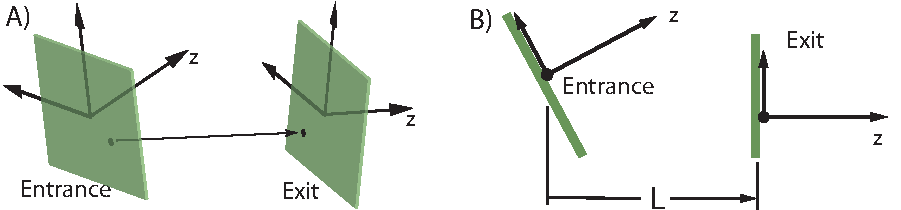
\includegraphics[width=5in]{patch.pdf}
  \caption[Patch Element.]
{A) A \vn{patch} element can align its exit face arbitrarily with respect to its entrance
face. B) The reference length of a \vn{patch} element is the longitudinal distance from
the entrance origin to the exit origin using the reference coordinates at the exit
end. Notice that while the length of the patch is defined with respect to the exit
coordinates, the offsets that define the position of the exit end coordinates are defined
with respect to the entrance coordinates.
}
  \label{f:patch}
\end{figure}

%-----------------

A \vn{patch} element shifts the reference orbit and time. Also see
\vn{floor_shift} (\sref{s:floor.ele}) and \vn{fiducial}
(\sref{s:fiducial}) elements.

General \vn{patch} element attributes are:
\begin{center}
\tt
\begin{tabular}{llll} \toprule
  {\sl Attribute Class}      & Section           & {\sl Attribute Class}      & Section         \\ \midrule
  Aperture limits            & \ref{s:limit}     & Offsets, pitches \& tilt   & \ref{s:offset}  \\ 
  Chamber wall               & \ref{s:wall}      & Reference energy           & \ref{s:energy}  \\
  Custom Attributes          & \ref{s:cust.att}  & Superposition              & \ref{s:super}   \\
  Description strings        & \ref{s:alias}     & Tracking \& transfer map   & \ref{c:methods} \\
  Length                     & \ref{s:l}         &                            &                 \\
  \bottomrule
\end{tabular}
\end{center}
\toffset
See \sref{s:list.patch} for a full list of element attributes.

\index{flexible}\index{e_tot_offset}
\index{x_offset}\index{y_offset}\index{z_offset}\index{tilt}
\index{x_pitch}\index{y_pitch}\index{t_offset}
Attributes specific to a \vn{patch} elements are:
\begin{example}
  x_offset        = <Real>  ! Exit face offset from Entrance.
  y_offset        = <Real>  ! Exit face offset from Entrance.
  z_offset        = <Real>  ! Exit face offset from Entrance.
  t_offset        = <Real>  ! Reference time offset.
  x_pitch         = <Real>  ! Exit face orientation from Entrance.
  y_pitch         = <Real>  ! Exit face orientation from Entrance.
  tilt            = <Real>  ! Exit face orientation from Entrance.
  e_tot_offset    = <Real>  ! Reference energy offset (eV).
  flexible        = <Logic> ! Default: False.
  l               = <Real>  ! Reference length. Dependent attribute (\sref{s:depend}). 
\end{example}
\index{x_offset}

A straight line element like a \vn{drift} or a \vn{quadrupole} has the the exit face
parallel to the entrance face. With a \vn{patch} element, the entrance and exit faces can
be arbitrarily oriented with respect to one another as shown in \fig{f:patch}A. The length
\vn{l} of a \vn{patch} is a dependent (\sref{s:depend}) parameter and is the longitudinal
($z$ component) distance from the entrance origin to the exit origin using the exit end
reference coordinates as shown in \fig{f:patch}B. See \sref{s:patch.prob} for a further
discussion on the coordinate system of a \vn{patch}. Notice that while the length of the
patche is defined with respect to the exit coordinates, the offsets that define the
position of the exit end coordinates are defined with respect to the entrance coordinates.

\index{rigid patch}\index{infleible patch}
\index{flexible patch}
There are two different ways the orientation of the exit face is
determined. Which way is used is determined by the setting of the
\vn{flexible} attribute.  With the \vn{flexible} attribute set to
\vn{False}, the default, The exit face of the \vn{patch} will be
determined from the offset, tilt and pitch attributes as described in
\sref{s:patch.coords}. This type of \vn{patch} is called ``rigid'' or
``inflexible'' since the geometry of the \vn{patch} is solely
determined by the \vn{patch}'s attributes and is independent of
everything else.  Example:
\begin{example}
  pt: patch, z_offset = 3.2   ! Equivalent to a drift
\end{example}

With \vn{flexible} set to \vn{True}, the exit face is taken to be the
reference frame of the entrance face of the next element in the
lattice. In this case, it must be possible to compute the reference
coordinates of the next element before the reference coordinates of
the \vn{patch} are computed. A \vn{flexible} \vn{patch} will have the
its offsets, pitches, and tilt as dependent parameters
(\sref{s:depend}) and these parameters will be computed. Here the
\vn{patch} is called ``flexible'' since the geometry of the patch will
depend upon the geometry of the rest of the lattice and, therefore, if
the geometry of the rest of the lattice is modified (is ``flexed''),
the geometry of the \vn{patch} will vary as well. See
Section~\sref{s:ex.erl} for an example.

If a \vn{flexible} patch is within a \vn{multipass} (\sref{s:multipass})
region (as opposed to being just outside a multipass region as in
the example in Section~\sref{s:ex.erl}), the offsets, pitches, and tilt
will be computed using the geometry of the first pass.

With \vn{bmad_standard} tracking (\sref{s:tkm}) A particle, starting
at the upstream face of the \vn{patch}, is propagated in a straight
line to the downstream face and the suitable coordinate transformation
is made to translate the particle's coordinates from the upstream
coordinate frame to the downstream coordinate frame
(\sref{s:patch.std}). In this case the \vn{patch} element can be
thought of as a generalized \vn{drift} element.

If there are magnetic or electric fields within the \vn{patch}, the
tracking method through the \vn{patch} must be set to either
\vn{runge_kutta} or \vn{custom}. Example:
\begin{example}
  pa2: patch, tracking_method = runge_kutta, field_calc = custom, 
              mat6_calc_method = tracking, ...
\end{example}
In order to supply a custom field when \vn{runge_kutta} tracking is
used, \vn{field_calc} (\sref{s:integ}) needs to be set to
\vn{custom}. In this case, custom code must be supplied for
calculating the fields as a function of position
(\sref{s:custom.ele}).

The \vn{e_tot_offset} attribute offsets the
reference energy:
\begin{example}
  E_tot_ref(exit) = E_tot_ref(entrance) + E_tot_offset (eV)
\end{example}
Setting the \vn{e_tot_offset} attribute will affect a particle's
$p_x$, $p_y$ and $p_z$ coordinates via \Eqs{ppp} and \eq{ppppp}.
Notice that \vn{e_tot_offset} does not affect a particle's actual
energy, it just affects the difference between the particle energy and
the reference energy. 

\vn{Important}: \bmad may apply the energy transformation either before or after the
coordinate transformation. This matters when the speed of the reference particle is less
than $c$. For this reason, and due to complications involving PTC, it is recommended to
use two patches in a row when both the orbit and energy are to be patched.

The \vn{t_offset} attribute offsets the reference time:
\begin{example}
  t_ref(exit) = t_ref(entrance) + t_offset + dt_travel_ref
\end{example}
where \vn{dt_transit_ref} is the time for the reference particle to
travel through the patch and \vn{dt_travel_ref} is the time the
reference particle takes to travel the patch. Setting the
\vn{t_offset} attribute will affect a particle's $z$ coordinate via
\Eqs{zbctt}. That is, \vn{t_offset} can be used to control the change
in the \vn{z} coordinate when tracking through a patch without
affecting the relative orientation of the exit edge of the patch
relative to the entrance end.

\vn{dt_travel_ref} in the above equation is computed by:
\begin{example}
  dt_travel_ref = L / beta_ref
\end{example}
Where \vn{L} is the length of the \vn{patch} as shown in \fig{f:patch}
and \vn{beta_ref} is the reference velocity/c at the exit end of the
element. That is, the reference energy offset is applied {\em before}
the reference particle is tracked through the patch. Since this point
can be confusing, it i recommended that a \vn{patch} element be split
into two consecutive patches if the \vn{patch} has finite \vn{l} and
\vn{E_tot_offset} values.

When a lattice branch contains both normally oriented and reversed
elements (\sref{s:ref.construct}), a \vn{patch}, or series of
\vn{patches}, which reflects the $z$ direction must be placed in
between. See \sref{s:ex.patch} for an example. Such a \vn{patch}, (or
patches) is called a \vn{reflection} \vn{patch}. See
Section~\sref{s:reflect.patch} for more details on how a reflection
patch is defined.

\index{wall}
Since the geometry of a \vn{patch} element is complicated,
interpolation of the chamber wall in the region of a patch follows
special rules. See section~\sref{s:wall.vacuum} for more details.

%-----------------------------------------------------------------
\section{Photon_Init}
\label{s:photon.init}
\index{photon_init|hyperbf}

A \vn{photon_init} element is used as a starting element for x-ray
tracking.  A \vn{photon_init} element can be used to define such
things as the initial energy spectrum and angular orientation. As
explained below, a \vn{photon_init} element can be a ``stand alone''
photon source or it can have an associated ``physical source''
element.

General \vn{photon_init} attributes are:
\begin{center}
\tt
\begin{tabular}{llll} \toprule
  {\sl Attribute Class}      & Section           & {\sl Attribute Class}      & Section         \\ \midrule
  Aperture limits            & \ref{s:limit}     & Length                     & \ref{s:l}       \\
  Chamber wall               & \ref{s:wall}      & Offsets, pitches \& tilt   & \ref{s:offset}  \\
  Custom Attributes          & \ref{s:cust.att}  & Reference energy           & \ref{s:energy}  \\ 
  Description strings        & \ref{s:alias}     & Tracking \& transfer map   & \ref{c:methods} \\ 
  \bottomrule
\end{tabular}
\end{center}
\toffset
See \sref{s:list.photon.init} for a full list of element attributes.

\index{x_half_length}\index{y_half_length}
Attributes specific to an \vn{photon_init} element are:
\begin{example}
  ds_slice                 = <Real>
  E_center                 = <Real>    ! Average initial photon energy (eV).
  E_center_relative_to_ref = <Logic>   ! E_center relative to reference E?
  e_field_x                = <Real>    ! Polarization. x & y = 0 -> random
  e_field_y                = <Real>
  energy_distribution      = <Switch>  ! Gaussian or uniform
  physical_source          = <String>  ! physical source of x-rays
  ref_wavelength                       ! Reference wavelength (\sref{s:energy}). Dependent attribute (\sref{s:depend}).
  sig_x                    = <Real>
  sig_y                    = <Real>
  sig_z                    = <Real>
  sig_vx                   = <Real>
  sig_vy                   = <Real>
  sig_E                    = <Real>    ! Initial photon energy width (eV).
  spatial_distribution     = <Switch>  ! Gaussian or uniform. 
  transverse_sigma_cut     = <Real>
  velocity_distribution    = <Switch>  ! Gaussian, spherical, or uniform. 
\end{example}

  \begin{description}
  \index{ds_slice}
  \item[\vn{ds_slice}] \Newline
Used when there is an associated physical source element. The physical
source element is sliced into pieces of thickness \vn{ds_slice} and
each slice is tested to see if photons from the slice can possibly
pass through the first aperture. When photons are generated, photons
will only be generated from slices where they have a hope of passing
through the first aperture. This makes the simulation more efficient.
The default value of \vn{ds_slice} is 0.01 meter.

  \index{E_center}
  \item[\vn{E_center}] \Newline
Average initial photon energy in eV. If \vn{E_center_relative_to_ref}
is set to True, \vn{E_center} will be relative to the reference
energy.

  \index{E_center_relative_to_ref}
  \item[\vn{E_center_relative_to_ref}] \Newline
\vn{E_center} an absolute value (referenced to zero) if
\vn{E_center_relative_to_ref} is set to False. With a setting of True
(the default), \vn{E_center} is taken to be with respect to the
reference energy (\sref{s:ref.energy}). That is, if set to True, the
center energy \vn{<E>} is
\begin{example}
  <E> = E_center + Reference_Energy
\end{example}

  \index{e_field_x}\index{e_field_y}
  \item[\vn{e_field_x}, \vn{e_field_y}] \Newline
Electric field component of initial photons in the $x$ and $y$ planes.
If both are set to 0 then a random field is chosen with unit intensity
$E_x^2 + E_y^2 = 1$.

  \index{energy_distribution}
  \item[\vn{energy_distribution}] \Newline
Sets the type of energy spectrum for emitted photons. If there is an
associated physical element then this parameter is ignored and the
energy distribution is calculated from the physical element. Possible
settings are:
\begin{example2}
  gaussian   ! Default
  uniform
\end{example2}
The \vn{gaussian} setting gives a Gaussian distribution with width
set by \vn{sig_E}. The \vn{uniform} setting gives a flat
distribution in the range:
\begin{example2}
  [-sig_E, sig_E]
\end{example2}

  \index{physical_source}
  \item[\vn{physical_source}] \Newline
Used to specify the ``physical'' source of the photons. See below for more details

  \index{sig_E}
  \item[\vn{sig_E}] \Newline
Energy width in eV. See \vn{energy_distribution} for more
details.

  \index{sig_vx}\index{sig_vy}
  \item[\vn{sig_vx, sig_vy}] \Newline
Width of emitted photons in $v_x/c$ and $v_y/c$ directions. See
\vn{velocity_distribution} for more details.

  \index{sig_x}\index{sig_y}\index{sig_z}
  \item[\vn{sig_x, sig_y, sig_z}] \Newline
Width of emitted photons in $x$, $y$ and $z$ directions. See
\vn{spatial_distribution} for more details.

  \index{spatial_distribution}
  \item[\vn{spatial_distribution}] \Newline
Sets spacial $(x, y, z)$ spectrum of emitted photons. If there is an
associated physical element then this parameter is ignored and the
energy distribution is calculated from the physical element. Possible
settings are:
\begin{example2}
  gaussian    ! Default
  uniform
\end{example2}
The \vn{gaussian} setting gives a Gaussian distribution with width
set by \vn{sig_E}. The \vn{uniform} setting gives a flat
distribution in the range:
\begin{example2}
  [-sig_E, sig_E]
\end{example2}
The \vn{gaussian} setting gives a Gaussian distribution with width
$\sigma$ where $sigma$ is 
\begin{example2}
  sig_x     ! for x distribution
  sig_y     ! for y distribution
  sig_z     ! for z distribution
\end{example2}
The \vn{uniform} setting gives a flat
distribution in the range: $[-\sigma, \sigma]$.

  \index{velocity_distribution}
  \item[\vn{velocity_distribution}] \Newline
Sets the transverse $(v_x/c, v_y/c)$ velocity spectrum of emitted
photons. If there is an associated physical element then this
parameter is ignored and the energy distribution is calculated from
the physical element. The longitudinal velocity is always computed to
make $v_x^2 + v_y^2 + v_z^2 = c^2$ Possible settings are:
\begin{example2}
  gaussian    ! Default
  spherical
  uniform
\end{example2}
The \vn{gaussian} setting gives a Gaussian distribution with width
$\sigma$ where $sigma$ is 
\begin{example2}
  sig_vx     for vx/c distribution
  sig_vy     for vy/c distribution
\end{example2}
The \vn{uniform} setting gives a flat distribution in the range:
$[-\sigma, \sigma]$.
The \vn{spherical} setting gives flat distribution in all directions.
  \end{description}

For the purposes of positioning the elements in the lattice around it,
a \vn{photon_init} element is considered to have zero length.

\vn{photon_init} elements are used in one of two modes: With or
without an associated physical source element specified by the
\vn{physical_source} attribute. Without an associated physical source,
the \vn{photon_init} element completely specifies the initial photon
distribution. With an associated physical source element, the photon
distribution is determined by the physical source but the shape of the
energy spectrum can be modified by setting attributes in the
\vn{photon_init} element. Example:
\begin{example}
  b05w: sbend, l = 3.2, angle = 0.1
  pfork: photon_fork, to_line = c_line, superimpose, ref = b05w, offset = 0.4
  bend_line: line = (..., b05w, ...)
  use bend_line

  c_line: line = (pinit, ...)
  c_line[e_tot] = 15e3
  pinit: photon_init, physical_source = 'b05w', sig_E = 2.1
\end{example}
In this example, the bend \vn{b05w} is a bend producing photons. It is
part of the line \vn{bend_line}. \vn{bend_line} also contains a
\vn{photon_fork} element named \vn{pfork} which branches to the line
\vn{c_line}. \vn{c_line} contains the \vn{photon_init} element
\vn{pinit} which references \vn{b03w} as the associated physical
source element. When photons are tracked, they are generated in
\vn{b05w} and then propagated to the \vn{pfork} fork.  After this they
are propagated through \vn{c_line}. The \vn{pinit} element acts like a
zero length \vn{marker} element when photons propagate through
it. That is, the \vn{pinit} element essentially serves to associate
\vn{c_line} with \vn{b03w} for the purposes of photon tracking. Also,
in this example, \vn{pinit} modifies the photon energy spectrum so
that only photons whose energy is within 2.1 eV are generated

It is important to note that in the above example, with the
\vn{photon_init} element having an associated physical source, the
setting of things like the spatial shape \vn{sig_z}, etc. in the
\vn{photon_init} element will be ignored.

%-----------------------------------------------------------------
\section{Quadrupole}
\label{s:quad}
\index{quadrupole|hyperbf}

A \vn{quadrupole} is a magnetic element with a linear field dependence
with transverse offset (\sref{s:mag.field}).

General \vn{quadrupole} attributes are:
\begin{center}
\tt
\begin{tabular}{llll} \toprule
  {\sl Attribute Class}      & Section           & {\sl Attribute Class}      & Section            \\ \midrule
  Aperture limits            & \ref{s:limit}     & Offsets, pitches \& tilt   & \ref{s:offset}     \\
  Chamber wall               & \ref{s:wall}      & Overlapping Fields         & \ref{s:overlap}    \\
  Description strings        & \ref{s:alias}     & Reference energy           & \ref{s:energy}     \\ 
  Fringe Fields              & \ref{s:fringe}    & Superposition              & \ref{s:super}      \\
  Hkick \& Vkick             & \ref{s:kick}      & Symplectify                & \ref{s:symp}       \\
  Is_on                      & \ref{s:is.on}     & Field Maps                 & \ref{s:fieldmap}   \\ 
  Length                     & \ref{s:l}         & Tracking \& transfer map   & \ref{c:methods}    \\ 
  Mag \& Elec multipoles     & \ref{s:multip}    &                            &                    \\
  \bottomrule
\end{tabular}
\end{center}
\toffset
See \sref{s:list.quadrupole} for a full list of element attributes.

\index{f1}\index{f2}
\index{k1}\index{b1_gradient}
Attributes specific to a \vn{quadrupole} element are:
\begin{example}
  b1_gradient    = <Real>    ! Field strength. (\sref{s:depend}).
  k1             = <Real>    ! Quadrupole strength.
  fq1            = <Real>    ! Soft edge fringe parameter.
  fq2            = <Real>    ! Soft edge fringe parameter.
 \end{example}

\index{tilt}
If the \vn{tilt} attribute is present without a value then a value of $\pi/4$
is used.

For a quadrupole with zero \vn{tilt} and a positive \vn{k1}, the
quadrupole is horizontally focusing and vertically defocusing
(\sref{s:mag.field}).

The \vn{fq1} and \vn{fq2} parameters are used to specify the
quadrupolar ``soft'' edge fringe. See \sref{s:q.soft} for more details.
The \vn{fringe_at} and \vn{fringe_type} settings (\sref{s:fringe})
determine if the fringe field is used in tracking.

Example:
\begin{example}
  q03w: quad, l = 0.6, k1 = 0.003, tilt  ! same as tilt = pi/4
\end{example}

%-----------------------------------------------------------------
\section{RFcavity}
\label{s:rfcav}
\index{rfcavity|hyperbf}

An \vn{rfcavity} is an RF cavity without acceleration generally used
in a storage ring. The main difference between an \vn{rfcavity} and an
\vn{lcavity} is that, unlike an \vn{lcavity}, the reference energy
(\sref{s:phase.space}) through an \vn{rfcavity} is constant.

General \vn{rfcavity} attributes are:
\begin{center}
\tt
\begin{tabular}{llll} \toprule
  {\sl Attribute Class}      & Section            & {\sl Attribute Class}      & Section            \\ \midrule
  Aperture limits            & \ref{s:limit}      & Offsets, pitches \& tilt   & \ref{s:offset}     \\
  Chamber wall               & \ref{s:wall}       & Overlapping Fields         & \ref{s:overlap}    \\
  Custom Attributes          & \ref{s:cust.att}   & Reference energy           & \ref{s:energy}     \\ 
  Description strings        & \ref{s:alias}      & RF Couplers                & \ref{s:rf.coupler} \\
  Field autoscaling          & \ref{s:autoscale}  & Superposition              & \ref{s:super}      \\
  Fringe Fields              & \ref{s:fringe}     & Symplectify                & \ref{s:symp}       \\
  Hkick \& Vkick             & \ref{s:kick}       & Field Maps                 & \ref{s:fieldmap}   \\
  Is_on                      & \ref{s:is.on}      & Tracking \& transfer map   & \ref{c:methods}    \\
  Length                     & \ref{s:l}          & Wakes                      & \ref{s:wakes}      \\
  \bottomrule
\end{tabular}
\end{center}
\toffset
See \sref{s:list.rfcavity} for a full list of element attributes.

\index{rf_frequency}\index{harmon}\index{voltage}\index{phi0}\index{phi0_multipass}\index{harmon_master}
Attributes specific to an \vn{rfcavity} are:
\begin{example}
  rf_frequency    = <Real>    ! Frequency
  harmon          = <Real>    ! Harmonic number
  voltage         = <Real>    ! Cavity voltage
  phi0            = <Real>    ! Cavity phase
  phi0_multipass  = <Real>    ! Phase variation with multipass
  gradient        = <Real>    ! Accelerating gradient (V/m). Dependent attribute (\sref{s:depend}).
\end{example}

The \vn{phi0} attribute here is identical to the \vn{lag} attribute of
\mad. The integrated energy kick felt by a particle, assuming no phase slippage, is 
\begin{example}
  dE = -e_charge * voltage * sin(\(2\,\pi\) * (\(\phi_\text{t}\) - \(\phi_\text{ref}\)))
\end{example}
\index{multipass}
where
\begin{example}
  \(\phi_\text{ref}\) = phi0 + phi0_multipass + phi0_autoscale
\end{example}
and $\phi_t$ is the part of the phase due to when the particle arrives
at the cavity and depends upon whether \vn{absolute time tracking} or 
\vn{relative time tracking} as discussed in \sref{s:rf.time}.

\vn{phi0_multipass} is only to be used to shift the phase with respect
to a \vn{multipass} lord. See \sref{s:multipass}. \vn{e_charge} is the
charge on an electron (Table~\ref{t:constants}). Notice that the
energy kick is independent of the sign of the charge of the particle

\vn{phi0_autoscale} and \vn{field_autoscale} are calculated by \bmad's auto-scale
module. See Section~\sref{s:autoscale} for more details. Autoscaling can be toggled on/off
by using the \vn{autoscale_phase} and \vn{autoscale_amplitude} toggles.

If \vn{harmon} is non--zero the \vn{rf_frequency} is calculated by
\begin{example}
  rf_frequency = harmon * c_light * beta0 / L_lattice 
\end{example}
where \vn{L_lattice} is the total lattice length and \vn{beta0} is the
velocity of the reference particle at the start of the lattice. After
the lattice has been read in, \vn{rf_frequency} will be the
independent variable (\sref{s:depend}).

Couplers (\sref{s:rf.coupler}) and HOM wakes (\sref{s:wakes}) can
be modeled. In addition, if a field map is specified
(\sref{s:fieldmap}), tracking using an integrator is possible.

\index{RF field map}
\index{runge_kutta!and field maps}\index{adaptive_runge_kutta!and field maps}
\index{boris!and field maps}\index{symp_lie_bmad!and field maps}
If a field map is specified (\sref{s:fieldmap}), tracking using an
integrator is possible. A field map is only used for \vn{runge_kutta},
\vn{adaptive_runge_kutta}, \vn{boris} and \vn{symp_lie_bmad} tracking
(\sref{s:tkm}).  Only the fundamental mode has an analytical formula
for the symplectic tracking. In the future, the other modes could be
used with \vn{symp_lie_bmad} tracking using a field expansion about
the centerline.

The \vn{cavity_type} is the type of cavity being simulated. Possible
settings are:
\begin{example}
  ptc_standard
  standing_wave    ! Default
  traveling_wave
\end{example}
The \vn{cavity_type} switch is ignored if a field map is used.

Example:
\begin{example}
  rf1: rfcav, l = 4.5, harmon = 1281, voltage = 5e6
\end{example}

%-----------------------------------------------------------------
\section{Sad_Mult}
\label{s:sad.mult}
\index{sad_mult|hyperbf}

A \vn{sad_mult} element is equivalent to a SAD\cite{b:sad} \vn{mult}
element. This element is a combination solenoid, multipole, bend, and
RF cavity.

General \vn{sample} attributes are:
\begin{center}
\tt
\begin{tabular}{llll} \toprule
  {\sl Attribute Class}      & Section           & {\sl Attribute Class}      & Section         \\ \midrule
  a$n$, b$n$ multipoles      & \ref{s:multip}    & Length                     & \ref{s:l}       \\
  Aperture limits            & \ref{s:limit}     & Offsets, pitches \& tilt   & \ref{s:offset}  \\
  Chamber wall               & \ref{s:wall}      & Reference energy           & \ref{s:energy}  \\ 
  Custom Attributes          & \ref{s:cust.att}  & Superposition              & \ref{s:super}   \\
  Description strings        & \ref{s:alias}     & Tracking \& transfer map   & \ref{c:methods} \\ 
  Fringe Fields              & \ref{s:fringe}    &                            &                 \\
  \bottomrule
\end{tabular}
\end{center}
\toffset
See \sref{s:list.sad.mult} for a full list of element attributes.

\index{angle}\index{bs_field}\index{e1}\index{e2}\index{eps_step_scale}
\index{f1}\index{f2}\index{g}\index{rf_frequency}\index{harmon}
\index{ks}\index{phi0}\index{rho}\index{voltage}\index{x_offset_mult}
\index{y_offset_mult}\index{x_pitch_mult}\index{y_pitch_mult}
\index{fringe_type}\index{kill_fringe}
Attributes specific to an \vn{sextupole} element are:
\begin{example}
  angle           = <Real>    ! Bend angle. A settable dependent variable (\sref{s:depend})
  bs_field        = <Real>    ! Solenoid field. SAD equivalent: BZ.
  e1, e2          = <Real>    ! Bend face angles.
  eps_step_scale  = <Real>    ! Step size scale. Default = 1. SAD equivalent: EPS.
  fq1             = <Real>    ! Quadrupole fringe integral. SAD equivalent: F1.
  fq2             = <Real>    ! Quadrupole fringe integral. SAD equivalent: F2.
  g               = <Real>    ! Bend strength 1/rho
  ks              = <Real>    ! Solenoid strength. 
  x_offset_mult   = <Real>    ! Mult component offset. SAD equivalent: DX.
  y_offset_mult   = <Real>    ! Mult component offset. SAD equivalent: DY.
  x_pitch_mult    = <Real>    ! Mult component pitch. SAD equivalent: DPX or CHI1.
  y_pitch_mult    = <Real>    ! Mult component pitch. SAD equivalent: DPY or CHI2.
  fringe_type     = <Switch>  ! Type of fringe. SAD equivalent: DISFRIN.
  fringe_at       = <Switch>  ! Where fringe is applied. SAD equivalent: FRINGE.
\end{example}

%  rf_frequency    = <Real>    ! Rf frequency (Hz). SAD equivalent: FREQ.
%  harmon          = <Real>    ! Harmonic number. SAD equivalent: HARM.
%  phi0            = <Real>    ! Cavity phase. SAD equivalent: PHI.
%  rho             = <Real>    ! Bend radius. A settable dependent variable (\sref{s:depend})
%  voltage         = <Real>    ! Cavity voltage. SAD equivalent: VOLT.

One difference between SAD and \bmad is that SAD defines the solenoid
field by what are essentially a set of marker elements so that the
solenoid field at a SAD \vn{mult} element is not explicitly declared
in the \vn{mult} element definition. \bmad, on the other hand,
requires a \vn{sad_mult} element to explicitly declare the solenoid
parameters.

Another difference between SAD and \bmad is that, within a solenoid,
the reference trajectory is aligned with the solenoid axis (and not
aligned with the axis of the elements within the solenoid region).

The SAD \vn{mult} element uses normal \vn{Kn} and skew \vn{KSn}
multipole components. The \bmad \vn{sad_mult} element used normal
\vn{an} and skew \vn{bn} multipole components. As can be seen from the
equations in \sref{s:mag.field}, there is a factor of $n!$ between the
two representations.

The \vn{fq1} and \vn{fq2} parameters are used to specify the
quadrupolar ``soft'' edge fringe. See \sref{s:q.soft} for more details.

The \vn{fringe_at} and \vn{fringe_type} settings (\sref{s:fringe})
determine if the fringe field is used in tracking.
The translation between these two switches and
the \vn{fringe} and \vn{disfrin} switches of SAD is:
\begin{center}
\tt
\begin{tabular}{ll|llll} 
\multicolumn{2}{c|}{\multirow{2}{*}{\textbf{[fringe, disfrin]}}}  & \multicolumn{4}{c}{fringe_at:} \\
              &                      & no_end     & entrance_end & exit_end   & both_ends$^*$ \\
\multirow{4}{*}{fringe_type:} 
              & none                 & [0, $\ne 0$] & [0, $\ne 0$]   & [0, $\ne 0$] & [0, $\ne 0$] \\
              & soft_edge_only       & [0, $\ne 0$] & [1, $\ne 0$]   & [2, $\ne 0$] & [3, $\ne 0$] \\
              & hard_edge_only$^*$   & [0, $\ne 0$] & -              & -            & [0, $= 0$]   \\
              & full                 & [0, $\ne 0$] & [1, $= 0$]     & [2, $= 0$]   & [3, $= 0$]   \\ 
  \bottomrule
\multicolumn{6}{l}{$^*$Default value.} \\
\end{tabular}
\end{center}
Each entry is the table is of the form [\vn{fringe}, \vn{disfrin}].
The ``-'' indicates that there is no equivalent setting in SAD.  The
\vn{soft_edge_only} fringe kick is a kick that is linear in the transverse
$(x, p_x, y, p_y)$ coordinates and comes from the finite width of the
quadrupolar fringe field. The width of the quadrupolar fringe field is
characterized by the \vn{f1} and \vn{f2} attributes. The
\vn{sad_nonlinear_only} fringe kick comes from the nonlinear part of
the quadrupolar field plus the fringes of the other multipoles.

Unlike other elements, the \vn{ds_step} and \vn{num_steps} attributes (\sref{s:integ}) of a \vn{sad_mult}
are dependent attributes (\sref{s:depend}) and are not directly settable. Rather these
attributes are calculated using \vn{SAD}'s own algorithm for setting the step size. To
vary the calculated step size for a single \vn{sad_mult} element, the attribute
\vn{eps_step_scale} may be set.  To vary the step size for all \vn{sad_mult} elements, the
global parameter \vn{bmad_com[sad_eps_scale]} (\sref{s:bmad.com}) may be set.
The default values for these parameters are:
\begin{example}
  eps_step_scale          = 1
  bmad_com[sad_eps_scale] = 5e-3
\end{example}

SAD conventions to be aware of when comparing SAD to Bmad:
\begin{itemize}
\item
A SAD \vn{rotate} or \vn{chi3} rotation is opposite to a \bmad \vn{tilt}
\item
SAD element offsets (\vn{dx}, \vn{dy}, \vn{dz}) are with respect to the entrance end
of the element as opposed to \bmad's convention of referencing to the element center.
\end{itemize}

%-----------------------------------------------------------------
\section{Sample}
\label{s:sample}
\index{sample|hyperbf}

A \vn{sample} element is used to simulate a material sample which is illuminated by x-rays.

General \vn{sample} attributes are:
\begin{center}
\tt
\begin{tabular}{llll} \toprule
  {\sl Attribute Class}      & Section           & {\sl Attribute Class}      & Section         \\
  Aperture limits            & \ref{s:limit}     & Offsets, pitches \& tilt   & \ref{s:offset}  \\ \midrule
  Chamber wall               & \ref{s:wall}      & Reference energy           & \ref{s:energy}  \\ 
  Custom Attributes          & \ref{s:cust.att}  & Surface Properties         & \ref{s:s.curve} \\
  Description strings        & \ref{s:alias}     & Superposition              & \ref{s:super}   \\
  Integration settings       & \ref{s:integ}     & Tracking \& transfer map   & \ref{c:methods} \\
  Length                     & \ref{s:l}         &                            &                 \\
  \bottomrule
\end{tabular}
\end{center}
\toffset
See \sref{s:list.sample} for a full list of element attributes.

This element is in development.

Attributes specific to an \vn{solenoid} element are:
\begin{example}
  mode       = <Switch> ! Reflection or transmission.
  material   = <type>   ! Type of material. \sref{s:cryst.list}
\end{example}

The \vn{mode} parameter can be set to:
\begin{example}
  reflection
  transmission
\end{example}
With \vn{mode} set to \vn{reflection}, photons will be back scattered
from the sample surface isotropically. In this case the material
properties will not matter. Additionally, a \vn{patch}
(\sref{s:patch}) element will be needed after the \vn{sample} element
to properly reorient the reference orbit.

With \vn{mode} set to \vn{transmission}, photons will be transmitted
through the sample. In this case \vn{material} will be used to
determine the attenuation and phase shift of the photons.

Example:
\begin{example}
  formula409: sample, x_limit = 10e-3, y_limit = 20e-3, mode = reflection
\end{example}

%-----------------------------------------------------------------
\section{Sextupole}
\label{s:sex}
\index{sextupole|hyperbf}

A \vn{sextupole} is a magnetic element with a quadratic field
dependence with transverse offset (\sref{s:mag.field}).

General \vn{sextupole} attributes are:
\begin{center}
\tt
\begin{tabular}{llll} \toprule
  {\sl Attribute Class}      & Section           & {\sl Attribute Class}      & Section         \\ \midrule
  Aperture limits            & \ref{s:limit}       & Mag \& Elec multipoles     & \ref{s:multip}     \\
  Chamber wall               & \ref{s:wall}        & Offsets, pitches \& tilt   & \ref{s:offset}     \\
  Custom Attributes          & \ref{s:cust.att}    & Overlapping Fields         & \ref{s:overlap}    \\
  Description strings        & \ref{s:alias}       & Reference energy           & \ref{s:energy}     \\ 
  Fringe Fields              & \ref{s:fringe}      & Superposition              & \ref{s:super}      \\
  Hkick \& Vkick             & \ref{s:kick}        & Symplectify                & \ref{s:symp}       \\
  Is_on                      & \ref{s:is.on}       & Field Maps                 & \ref{s:fieldmap}   \\
  Length                     & \ref{s:l}           & Tracking \& transfer map   & \ref{c:methods}    \\ 
  \bottomrule
\end{tabular}
\end{center}
\toffset
See \sref{s:list.sextupole} for a full list of element attributes.

\index{k2}
\index{b2_gradient}
Attributes specific to an \vn{sextupole} element are:
\begin{example}
  k2          = <Real>   ! Sextupole strength.
  b2_gradient = <Real>   ! Field strength. (\sref{s:depend}).
\end{example}

The \vn{bmad_standard}
calculation treats a sextupole using a kick--drift--kick model.

If the \vn{tilt} attribute is present without a value then a value of 
$\pi/6$ is used.
Example:
\begin{example}
  q03w: sext, l = 0.6, k2 = 0.3, tilt  ! same as tilt = pi/6
\end{example}

%-----------------------------------------------------------------
\section{Solenoid}
\label{s:sol}
\index{solenoid|hyperbf}

A \vn{solenoid} is an element with a longitudinal magnetic field.

General \vn{solenoid} attributes are:
\begin{center}
\tt
\begin{tabular}{llll} \toprule
  {\sl Attribute Class}      & Section             & {\sl Attribute Class}      & Section            \\ \midrule
  Aperture limits            & \ref{s:limit}       & Mag \& Elec multipoles     & \ref{s:multip}     \\
  Chamber wall               & \ref{s:wall}        & Offsets, pitches \& tilt   & \ref{s:offset}     \\
  Custom Attributes          & \ref{s:cust.att}    & Overlapping Fields         & \ref{s:overlap}    \\
  Description strings        & \ref{s:alias}       & Reference energy           & \ref{s:energy}     \\ 
  Fringe Fields              & \ref{s:fringe}      & Superposition              & \ref{s:super}      \\
  Hkick \& Vkick             & \ref{s:kick}        & Symplectify                & \ref{s:symp}       \\
  Is_on                      & \ref{s:is.on}       & Field Maps                 & \ref{s:fieldmap}   \\
  Length                     & \ref{s:l}           & Tracking \& transfer map   & \ref{c:methods}    \\ 
  \bottomrule
\end{tabular}
\end{center}
\toffset
See \sref{s:list.solenoid} for a full list of element attributes.

\index{ks}
\index{bs_gradient}
Attributes specific to an \vn{solenoid} element are:
\begin{example}
  ks         = <Real>   ! Solenoid strength.
  bs_field   = <Real>   ! Field strength. (\sref{s:depend}).
\end{example}

The \vn{bmad_standard} tracking model (\sref{s:tkm}) uses a ``hard
edge'' model where an impulse kick is applied at the entrance and exit
ends of the element due to the fringe fields there.

Example:
\begin{example}
  cleo_sol: solenoid, l = 2.6, ks = 1.5e-9 * parameter[e_tot]
\end{example}

%-----------------------------------------------------------------
\section{Sol_Quad}
\label{s:sq}
\index{sol_quad|hyperbf}

A \vn{sol_quad} is a combination solenoid/quadrupole.

General \vn{sol_quad} attributes are:
\begin{center}
\tt
\begin{tabular}{llll} \toprule
  {\sl Attribute Class}      & Section             & {\sl Attribute Class}      & Section            \\ \midrule
  Aperture limits            & \ref{s:limit}       & Mag \& Elec multipoles     & \ref{s:multip}     \\
  Chamber wall               & \ref{s:wall}        & Offsets, pitches \& tilt   & \ref{s:offset}     \\
  Custom Attributes          & \ref{s:cust.att}    & Overlapping Fields         & \ref{s:overlap}    \\
  Description strings        & \ref{s:alias}       & Reference energy           & \ref{s:energy}     \\ 
  Fringe Fields              & \ref{s:fringe}      & Superposition              & \ref{s:super}      \\
  Hkick \& Vkick             & \ref{s:kick}        & Symplectify                & \ref{s:symp}       \\
  Is_on                      & \ref{s:is.on}       & Field Maps                 & \ref{s:fieldmap}   \\
  Length                     & \ref{s:l}           & Tracking \& transfer map   & \ref{c:methods}    \\ 
  \bottomrule
\end{tabular}
\end{center}
\toffset
See \sref{s:list.sol.quad} for a full list of element attributes.

\index{k1}\index{ks}\index{bs_field}\index{b1_gradient}
Attributes specific to a \vn{sol_quad} element are:
\begin{example}
  k1          = <Real>    ! Quadrupole strength.
  ks          = <Real>    ! Solenoid strength.
  bs_field    = <Real>    ! Solenoid Field strength.
  b1_gradient = <Real>    ! Quadrupole Field strength.
\end{example}

Example:
\begin{example}
  sq02: sol_quad, l = 2.6, k1 = 0.632, ks = 1.5*beam[energy]
\end{example}

%-----------------------------------------------------------------
\section{Taylor}
\label{s:taylor}
\index{taylor|hyperbf}

A \vn{taylor} is a Taylor map (\sref{s:taylor.phys}). This can be used
in place of the \mad \vn{matrix} element.

General \vn{taylor} attributes are:
\begin{center} 
\tt
\begin{tabular}{llll} \toprule
  {\sl Attribute Class}      & Section          & {\sl Attribute Class}      & Section         \\ \midrule
  Aperture limits            & \ref{s:limit}    & Offsets \& tilt            & \ref{s:offset}  \\
  Custom Attributes          & \ref{s:cust.att} & Reference energy           & \ref{s:energy}  \\
  Description strings        & \ref{s:alias}    & Superposition              & \ref{s:super}   \\
  Is_on                      & \ref{s:is.on}    & Symplectify                & \ref{s:symp}    \\
  Length                     & \ref{s:l}        & Tracking \& transfer map   & \ref{c:methods} \\

  \bottomrule
\end{tabular}
\end{center}
\toffset
See \sref{s:list.taylor} for a full list of element attributes.

Attributes specific to a \vn{taylor} element are:
\begin{example}
  ref_orbit = (<x>, <px>, <y>, <py>, <z>, <pz>)     ! Reference orbit.
  \{<out>: <coef>, <e1> <e2> <e3> <e4> <e5> <e6>\}  ! Taylor term. First form.
  \{<out>: <coef> | <n1> <n2> ...\}                 ! Taylor term. Second form.
  tt<out><n1><n2>...  = <Coef>                      ! Taylor term. Third form.
\end{example}

For historical reasons, there are three differnt forms that can be used to specify a
taylor term.  Notice that the first form (above) uses a comma ``,'' to separate the
\vn{<coef>} from \vn{<e1>}, while the second form uses a vertical bar ``|'' to separate
\vn{<coef>} from \vn{<n1>}.

A Taylor term has a coefficient \vn{<coef>} which is a real number,
integer exponents \vn{<e1>}, \vn{<n1>}, etc., and \vn{<out>} signifies
which output variable the Taylor term is associated with.  For orbital
phase space variables \vn{<Out>} is an integer in the range 1 to 6
with \vn{<out>} = 1 for $x$, etc. For terms associated with spin,
\vn{<out>} is a two character string with each character being
one of ``\vn{x}'', ``\vn{y}'', or ``\vn{z}''. 

For orbital phase space variables a term in a Taylor map is of the form
\Begineq
  x_j(\Out) = C \cdot \Pi_{i = 1}^6 \, x_i^{e_i}(\In)
\Endeq
where $\Bf x = (x, p_x, y, p_y, z, p_z)$. A term in a Taylor map can
be specified by one of two forms as shown above. The first form specifies
the six exponents $e_i$ using the integers \vn{<e1>} corresponding to
$e_1$, \vn{<e2>} corresponding to $e_2$, etc.  For example, a term in
a Taylor map that was
\Begineq
  p_y(\Out) = 2.73 \cdot y^2(\In) \, p_z(\In)
\Endeq
would be written as
\begin{example}
  \{4: 2.73, 0 0 2 0 0 1\} or
\end{example}

The second form for specifying a Taylor term uses a set of integers \vn{<n1>},
\vn{<n2>}, etc. Each integer must be between 1 and 6 inclusive. The value of 
the $i$\Th exponent $e_i$ is equal to the number of integers that are equal
to $i$. For example, the term of the above example would be written using
the second form as
\begin{example}
  \{4: 2.73 | 336\}
\end{example}
Notice that with the second form, spaces between exponent terms is optional.

The third form is like the second form. For example, the term of the above examples
would be written unsing the third form as:
\begin{example}
  tt4336 = 2.73
\end{example}

By default a \vn{taylor} element starts out as the unit map. 
That is, a \vn{taylor} element starts with the following 6 terms
\begin{example}
  \{1: 1.0, 1 0 0 0 0 0\}
  \{2: 1.0, 0 1 0 0 0 0\}
  \{3: 1.0, 0 0 1 0 0 0\}
  \{4: 1.0, 0 0 0 1 0 0\}
  \{5: 1.0, 0 0 0 0 1 0\}
  \{6: 1.0, 0 0 0 0 0 1\}
\end{example}
Which is equivalent to
\begin{example}
  \{1: 1.0 | 1\}
  \{2: 1.0 | 2\}
  \{3: 1.0 | 3\}
  \{4: 1.0 | 4\}
  \{5: 1.0 | 5\}
  \{6: 1.0 | 6\}
\end{example}

For spin, a Taylor map is associated with one of the components in the
3x3 spin map matrix (\sref{s:spin.map}). An individual Taylor term is
of the form
\Begineq
  S_j(\Out) = C \cdot \Pi_{i = 1}^6 \, x_i^{e_i}(\In) \, S_k(\In)
\Endeq
For example
\begin{example}
  \{xz: 0.43 | 13 \}
\end{example}
is equivalent to
\Begineq
  S_x(\Out) = 0.43 \cdot x(\In) \, y(\In) \, S_z(\In)
\Endeq

A term in a \vn{taylor} element will override any previous term
with the same \vn{out} and \vn{e1} through \vn{e6} indexes. For example the term:
\begin{example}
  tt: Taylor, \{1: 4.5, 1 0 0 0 0 0\} 
\end{example}
will override the default \vn{\{1: 1.0, 1 0 0 0 0 0\}} term.

The \vn{l} length attribute does not affect phase space coordinates
but will affect the longitudinal $s$ position of succeeding elements
and will affect the time it takes a particle to track through the
element.

The \vn{ref_orbit} attribute specifies the phase space $(x, px, y, py, z, pz)$ reference
orbit at the start of the element used to construct the Taylor map. The reference orbit
only has an effect when used in conjunction with PTC (\sref{c:ptc}). In this case, PTC
uses the reference orbit when doing such things as normal form analysis. Note: when
converting the map from \bmad to PTC, the interface routine will convert from Bmad phase
space coordinates to PTC phase space coordinates and will convert the map to using the
reference orbit as the map zero orbit. This does not affect tracking but will affect map
analysis.

A \vn{taylor} element that is ``turned off'' (\vn{is_on} attribute set to False), is
considered to be like a \vn{marker} element. That is, the orbit and twiss parameters are
unchanged when tracking through a \vn{taylor} element that is turned off.

Example \vn{taylor} element definition:
\begin{example}
  tt: Taylor, \{4:  2.7, 0 0 2 0 0 1\}, \{2:  1.9 | 1 1 2\},
              \{xz: 0.43 | 2 \}, ..., 
              ref_orbit = (0.01, 0.003, 0.002, 0.001, 0.0, 0.2)
\end{example}

%-----------------------------------------------------------------
\section{Wiggler and Undulator} 
\label{s:wiggler}
\index{wiggler|hyperbf} 
\index{undulator|hyperbf} 

A \vn{wiggler} or \vn{undulator} element is basically a periodic array of alternating bends.
The only difference between \vn{wigglers} and \vn{undulators} is in the x-ray emission spectrum.
Charged particle tracking will be the same. 

Henceforth, the term ``wiggler'' will denote either a \vn{wiggler} or \vn{undulator}

General \vn{wiggler} attributes are:
\begin{center}
\tt
\begin{tabular}{llll} \toprule
  {\sl Attribute Class}      & Section             & {\sl Attribute Class}      & Section            \\ \midrule
  Aperture limits            & \ref{s:limit}       & Mag \& Elec multipoles     & \ref{s:multip}     \\
  Chamber wall               & \ref{s:wall}        & Offsets, pitches \& tilt   & \ref{s:offset}     \\
  Custom Attributes          & \ref{s:cust.att}    & Overlapping Fields         & \ref{s:overlap}    \\
  Description strings        & \ref{s:alias}       & Reference energy           & \ref{s:energy}     \\ 
  Fringe Fields              & \ref{s:fringe}      & Superposition              & \ref{s:super}      \\
  Hkick \& Vkick             & \ref{s:kick}        & Symplectify                & \ref{s:symp}       \\
  Is_on                      & \ref{s:is.on}       & Field Maps                 & \ref{s:fieldmap}   \\
  Length                     & \ref{s:l}           & Tracking \& transfer map   & \ref{c:methods}    \\ 
  \bottomrule
\end{tabular}
\end{center}
\toffset
See \sref{s:list.wiggler} for a full list of element attributes.

There are two types of wigglers. Those that that are described using a
magnetic field map (``map type'') and those that are described
assuming a periodic field (``periodic type''). 

%-----------------------------------------------------
\subsection{Map\_Type Wigglers}
\label{s:wiggler.map}

The \vn{map type} wigglers are modeled using the Cartesian mode
decomposition of Sec.~\sref{s:cart.map}. 

\index{polarity}
\index{term (for a wiggler)}
Attributes specific to a \vn{map type} \vn{wiggler} element are:
\begin{example}
  b_max    = <Real>   ! Maximum magnetic field (in T) on the wiggler centerline. 
                      !   Dependent attribute (\sref{s:depend}).
  polarity = <Real>   ! For scaling the field.
\end{example}

The \vn{polarity} value is used to scale the magnetic field. By
default, \vn{polarity} has a value of 1.0.  Example:
\begin{example}
  wig1: wiggler, l = 1.6, polarity = -1, cartesian_map = \{...\}
\end{example}

The \vn{b_max} attribute for a \vn{map type} \vn{wiggler} is the
maximum field computed for \vn{polarity} = 1.

There is no \vn{bmad_standard} tracking for a \vn{map_type}
\vn{wiggler}. \vn{symp_lie_bmad} type tracking is discussed in \sref{s:symp.track}

%-----------------------------------------------------
\subsection{Old Map\_Type Wigglers Syntax}
\label{s:old.wiggler}

When the wiggler model was first developed, the definition of the field was somewhat
different and there was a special syntax for specifying the field. The old syntax looked
like
\Begineq
  \text{term(i)} = \{C, k_x, k_y, k_z, \phi_z \}
\Endeq
Example:
\begin{example}
  wig1: wiggler, l = 1.6, 
        term(1) = \{0.03, 3.00, 4.00, 5.00, 0.63\},
        term(2) = ...
\end{example}

The old definition used only the three forms corresponding to the \vn{cartesian_map}
\vn{y} family (\sref{s:cart.map.phys}) with $x_0 = y_0 = 0$. There was also a different
normalization convention. The old style \vn{hyper-y} form was
\begin{alignat}{5}
  B_x &= -& C \, &\dfrac{k_x}{k_y} & \sin(k_x x) \sinh(k_y y) \cos(\kzz) &\CRNEG
  B_y &=  & C \, &                 & \cos(k_x x) \cosh(k_y y) \cos(\kzz) &\qquad \text{! Old style} \CRNEG
  B_s &= -& C \, &\dfrac{k_z}{k_y} & \cos(k_x x) \sinh(k_y y) \sin(\kzz) &\label{f1} \\
  & \makebox[1pt][l]{with $k_y^2 = k_x^2 + k_z^2$ .} &&&&  \nonumber
\end{alignat}
The old style \vn{hyper-xy} form was
\begin{alignat}{5}
  B_x &=  & C \, &\dfrac{k_x}{k_y} & \sinh(k_x x) \sinh(k_y y) \cos(\kzz) &\CRNEG
  B_y &=  & C \, &                 & \cosh(k_x x) \cosh(k_y y) \cos(\kzz) &\qquad \text{! Old style} \CRNEG
  B_s &= -& C \, &\dfrac{k_z}{k_y} & \cosh(k_x x) \sinh(k_y y) \sin(\kzz) &\label{f2} \\
  & \makebox[1pt][l]{with $k_y^2 = k_z^2 - k_x^2$ ,} &&&&  \nonumber
\end{alignat}
The old style \vn{hyper_x} form was
\begin{alignat}{5}
  B_x &=  & C \, &\dfrac{k_x}{k_y} & \sinh(k_x x) \sin(k_y y) \cos(\kzz) &\CRNEG
  B_y &=  & C \, &                 & \cosh(k_x x) \cos(k_y y) \cos(\kzz) &\qquad \text{! Old style} \CRNEG
  B_s &= -& C \, &\dfrac{k_z}{k_y} & \cosh(k_x x) \sin(k_y y) \sin(\kzz) &\label{f3} \\
  & \makebox[1pt][l]{with $k_y^2 = k_x^2 - k_z^2$ .} &&&& \nonumber
\end{alignat}
The correspondence between $C$ in the above equations and $A$ in the new equations is
given by comparing \Eqs{f1}, \eq{f2}, and \eq{f3} with \Eqs{family.y}.

When the {cartesian_map} constract was being developed, an intermediate hybrid syntax was used defined:
\Begineq
  term(i) = \{A, k_x, k_y, k_z, x_0, y_0, \phi_z, \text{family}\}
\Endeq
The parameters here directly correspond to the \vn{cartesian_map} forms (see \Eqs{cm1} through \eq{bsq}).

For example, the old style syntax:
\begin{example}
  term(1) = \{0.03*4/5, 3.00, 4.00, 5.00, 0.63 \}    ! Old style
\end{example}
is equivalent to:
\begin{example}
  term(2) = \{0.03, 3.00, 4.00, 5.00, 0, 0, 0.63, y\}  ! Hybrid style
\end{example}

Note: When converting from the old or hybrid styles to \vn{cartesian_map}, the
\vn{field_calc} parameter must be set to \vn{fieldmap}.

%-----------------------------------------------------
\subsection{Periodic\_Type Wiggler Element Tracking}
\label{s:wiggler.periodic}

For the \vn{periodic type} wigglers the attributes are: 
\index{b_max}\index{n_pole}
\index{k1}\index{rho}
\begin{example}  
  b_max    = <Real>  ! Maximum magnetic field (in T) on the wiggler centerline. 
  l_pole   = <Real>  ! Wiggler pole length. The period is then 2 * l_pole.
  n_pole   = <Real>  ! The number of poles (L / L_POLE). 
                     !   A settable Dependent attribute (\sref{s:depend}).
\end{example}

Example:
\begin{example}
  wig2: wiggler, l = 1.6, b_max = 2.1, n_pole = 7  ! periodic type wiggler
\end{example}

The type of wiggler is determined by whether there are \vn{term(i)}
terms. If present, the wiggler is classed as a \vn{map type}.

Note: When using Taylor maps and symplectic tracking with a
\vn{periodic} type wiggler, the number of poles must be even.

The horizontal motion looks like a drift with a superimposed
sinusoidal oscillation. It is assumed that there is an integer number
of periods in the oscillation so that the exit horizontal coordinates
can be calculated from the initial coordinates using the equations for
a drift. The vertical motion is a quadratic superimposed with a
octupole. Vertical motion is calculated using a kick-drift-kick model.

\vn{Periodic type} wigglers use a simplified model where the magnetic
field components are
\begin{alignat}{1}
  B_y &= \hphantom{-} B_{\max} \, \cosh(k_z \, y) \, \cos(k_z \, z + \phi_z) \CRNO
  B_z &= -B_{\max} \, \sinh(k_z \, y) \, \sin(k_z \, z + \phi_z) 
  \label{bbkykz}
\end{alignat}
where $B_{\max}$ is the maximum field on the centerline and $k$ is
given in terms of the pole length (\vn{l_pole}) by
\Begineq
  k_z = \frac{\pi}{l_{\text{pole}}}
\Endeq
This type of wiggler has infinitely wide poles. With
\vn{bmad_standard} tracking and transfer matrix calculations the
vertical focusing is assumed small so averaged over a period the
horizontal motion looks like a drift and the vertical motion is
modeled as a combination focusing quadrupole and focusing octupole
giving a kick\cite{b:corbett}
\Begineq
  \frac{dp_y}{dz} = k_1 \left( y + \frac{2}{3} \, k_z^2 \, y^3 \right)
\Endeq
where
\begin{alignat}{1}
  k_1 &= \frac{-1}{2} \, \left( \frac{e \, B_{\max}}{P_0 \, (1 + p_z)} \right)^2 
\end{alignat}
with $k_1$ being the linear focusing constant. For radiation
calculations the true horizontal trajectory with $y = 0$ is needed
\Begineq
  x = \frac{\sqrt{2 \, |k_1|}}{k_z^2} \, \cos (k_z \, z)
\Endeq

With \vn{periodic type} wigglers and \vn{bmad_standard}
tracking, the phase $\phi_z$ in \Eqs{bbkykz} is irrelevant. When the
tracking involves Taylor maps and symplectic integration, the phase is
important. Here the phase is chosen so that $B_y$ is symmetric about
the center of the wiggler
\Begineq
  \phi_z = \frac{-k_y \, L}{2}
\Endeq
With this choice, a particle that enters the wiggler on-axis will
leave the wiggler on-axis provided there is an even number of poles.

When using a tracking through a periodic wiggler with a tracking
method that integrates through the magnetic field (\sref{s:integ}),
The magnetic field is approximated using a single wiggler \vn{term} as
if the wiggler were a \vn{map type} wiggler. This wiggler model has
unphysical end effects and will give results that are different from
the results obtained when using the \vn{bmad_standard} tracking
method. 

Example:
\begin{example}
  wig_w: wiggler, l = 2.3, b_max = 2.3, l_pole = 6
\end{example}

%-----------------------------------------------------
\subsection{Common Wiggler Parameters}

Tracking a particle through a wiggler is always done so that
if the particle starts on-axis with no momentum offsets, there is no
change in the $z$ coordinate even though the actual trajectory through
the wiggler does not follow the straight line reference trajectory.

\index{x_ray_line_len}
both types of wigglers have the following attributes:
\begin{example}
  x_ray_line_len = <Real>
  polarity       = <Real> ! Used to scale the field strength.
  k1                      ! Vertical focusing strength. Dependent attribute (\sref{s:depend}).
  rho                     ! Bending radius. Dependent attribute (\sref{s:depend}).
\end{example}
\vn{x_ray_line_len} is the length of an associated x-ray synchrotron
light line measured from the exit end of the element. This is used for
machine geometry calculations and is irrelevant for lattice
computations.
